%% ----------------------------------------------------------------
%% Tesis.tex -- Archivo principal
%% ---------------------------------------------------------------- 

% Asignar el documento
\documentclass[letterpaper, 12pt, twoside]{TesisUNAM}  % Usa el tipo de documento "ThesisUNAM"

% Include any extra LaTeX packages required
\usepackage[square, numbers, comma, sort&compress]{natbib}  % Use the "Natbib" style for the references in the Bibliography
\usepackage{amsmath}
\usepackage{amssymb}
\usepackage{listings} % para escribir código
\usepackage{xcolor}
\usepackage[spanish]{babel}
%\usepackage{algorithm}
%\usepackage{algpseudocode}
\usepackage[ruled,vlined,linesnumbered,spanish,onelanguage]{algorithm2e}
\usepackage{graphicx}
\usepackage{booktabs}
\usepackage{float} % Necesario para la opción H
\usepackage{longtable}

\definecolor{codegreen}{rgb}{0,0.6,0}
\definecolor{codegray}{rgb}{0.5,0.5,0.5}
\definecolor{codepurple}{rgb}{0.58,0,0.82}
\definecolor{backcolour}{rgb}{0.95,0.95,0.92}

\lstdefinestyle{mystyle}{
    backgroundcolor=\color{backcolour},   
    commentstyle=\color{codegreen},
    keywordstyle=\color{magenta},
    numberstyle=\tiny\color{codegray},
    stringstyle=\color{codepurple},
    basicstyle=\ttfamily\footnotesize,
    breakatwhitespace=false,         
    breaklines=true,                 
    captionpos=b,                    
    keepspaces=true,                 
    numbers=left,                    
    numbersep=5pt,                  
    showspaces=false,                
    showstringspaces=false,
    showtabs=false,                  
    tabsize=2
}

\lstset{style=mystyle}

\title{Análisis de Modelos de Redes Neuronales en la predicción de precios de las acciones en la BMV}
\author{Miguel Angel Liera Montaño}
\modalidad{T E S I S}
\tituloprofesional{Licenciado en Ciencias de la Computación}
\facultad{Facultad de Ciencias}
\escudofacultad{EscudoFCiencias}
\supervisor{Dra. Verónica Esther Arriola Ríos}

\begin{document}
\frontmatter	  % Begin Roman style (i, ii, iii, iv...) page numbering
\maketitle

% Si numeración ni encabezados
\pagestyle{empty}

% Dedicatoria
\dedicatory{A Thayla, Andrea y Alicia}

% Agradecimientos
\acknowledgements{
    Quisiera experesar mis más profundos agradecimientos a la Dra. Arriola Ríos
    , mi asesora, quien fue mi guía y gracias a su experiencia, conocimiento y paciencia pude completar esta trabajo. También a mis sinodales, el Dr. en Lingüística Mijangos de la Cruz, el M. en C. Hernández López, la Dra. Naranjo Albarrán y al M. en I. Torres Bello quienes con su saber y apoyo me ayudaron a enriquecer el presente proyecto. Mi especial gratitud a Dra. Gasca Soto por motivarme a seguir con este.

    A mi hermana Andrea agradezco su apoyo y amor, sin el cuál no podría haberme convertido en la persona que soy hoy, a mi sobrina Thayla por su alegría que me motiva a seguir y a mis padres Lilian y Luis por su soporte. A Alicia, mi novia, por su enorme amor durante todo este tiempo.

    Muchas gracias a todos mis compañeros y amigos, especialmente a Angel Peña, a quien agradezco por haber elegido la profesión cientifica. A Gerardo Martinez, Oswaldo Sanchez y Victor Cuevas quienes han estado presentes en mi vida desde la escuela preparatoria y me han acompañado en este proceso. A Natalia quien agradezco su cariño durante mis estudios. A Fausto Hernandez, Rodrigo Arévalo, Santiago Arrollo, Diana Hernández y Berenice Calvario por su hermandad durante estos últimos años. 
 %Los agradecimientos van aquí\ldots
 
 %Para quitar los marcos alrededor de la página comentar la línea 117 en TesisUNAM.cls que dice \textit{$\backslash$usepackage\{showframe\}}.
}

% Inicia el contedio
\pagestyle{fancy} 

%% ----------------------------------------------------------------
\tableofcontents  % Write out the Table of Contents

%% ----------------------------------------------------------------
\listoffigures  % Write out the List of Figures

%% ----------------------------------------------------------------
\listoftables  % Write out the List of Tables

%% ----------------------------------------------------------------
\setstretch{1.5}  % Set the line spacing to 1.5, this makes the following tables easier to read
\clearpage  % Start a new page
\listofsymbols{ll}  % Include a list of Abbreviations (a table of two columns)
{
% \textbf{Acronym} & \textbf{W}hat (it) \textbf{S}tands \textbf{F}or \\
\textbf{FT} & \textbf{F}ourier \textbf{T}ransform \\
\textbf{STFT} & \textbf{S}hort \textbf{T}ime \textbf{F}ourier \textbf{T}ransform\\
\textbf{WFT} & \textbf{W}indowed \textbf{F}ourier \textbf{T}ransform\\
\textbf{WT} & \textbf{W}avelet \textbf{T}ransform\\
\textbf{CWT} & \textbf{C}ontinous \textbf{W}avelet \textbf{T}ransform\\
\textbf{DWT} & \textbf{D}iscrete \textbf{W}avelet \textbf{T}ransform\\
\textbf{ANNs} & \textbf{A}rtificial \textbf{N}eural \textbf{N}etworks\\
\textbf{ARIMA} & \textbf{A}utoregressive \textbf{I}ntegrated \textbf{M}oving \textbf{A}verage\\
\textbf{ARMA} & \textbf{A}utoregressive \textbf{M}oving \textbf{A}verage\\
\textbf{SVMs} & \textbf{S}upport \textbf{V}ector \textbf{M}achines\\
\textbf{MSE} & \textbf{M}ean \textbf{S}quare \textbf{E}rror\\
\textbf{MAE} & \textbf{M}ean \textbf{A}bsolute \textbf{E}rror\\
\textbf{GD} & \textbf{G}radient \textbf{D}escent\\
\textbf{SGD} & \textbf{S}tochastic \textbf{G}radient \textbf{D}escent\\
\textbf{ADAM} & \textbf{A}daptative \textbf{M}oment \textbf{E}stimation\\
\textbf{LM} & \textbf{L}evenberg-\textbf{M}arquardt\\
\textbf{NARNNs} & \textbf{N}ot linear
\textbf{A}utorregresive \textbf{N}eural \textbf{N}etworks\\
\textbf{RNNs} & \textbf{R}ecurretn \textbf{N}eural \textbf{N}etworks\\
\textbf{RMLP} & \textbf{R}ecurrent \textbf{M}ulti\textbf{L}ayer \textbf{Perceptron}\\
\textbf{LSTM} & \textbf{L}ong \textbf{S}hort-\textbf{T}erm \textbf{Memory}\\
\textbf{GRU} & \textbf{G}ated \textbf{R}ecurrent \textbf{U}nit\\
\textbf{LTR} & \textbf{L}inea de \textbf{T}iempo \textbf{R}etrasado\\
\textbf{RMSE} & \textbf{R}ooted \textbf{M}ean \textbf{S}quared \textbf{E}rror\\
\textbf{MAPE} & \textbf{M}ean \textbf{A}verage \textbf{P}ercentage \textbf{E}rror\\
\textbf{DS} & \textbf{D}irectional \textbf{S}ymmetry\\
\textbf{FD} & \textbf{F}actor de \textbf{D}ecaimiento\\
\textbf{GNNs} & \textbf{Graph} \textbf{Neural} \textbf{Networks}\\
}

%% ----------------------------------------------------------------
%\clearpage  % Start a new page
%\listofconstants{lrcl}  % Include a list of Physical Constants (a four column table)
%{
% Constant Name & Symbol & = & Constant Value (with units) \\
%Speed of Light & $c$ & $=$ & $2.997\ 924\ 58\times10^{8}\ \mbox{ms}^{-\mbox{s}}$ (exact)\\

%}

%% ----------------------------------------------------------------
%\clearpage  %Start a new page
%\listofnomenclature{lll}  % Include a list of Symbols (a three column table)
%{
% symbol & name & unit \\
%a$ & distance & m \\
%$P$ & power & W (Js$^{-1}$) \\
%& & \\ % Gap to separate the Roman symbols from the Greek
%$\omega$ & angular frequency & rads$^{-1}$ \\
%}



\mainmatter	  % Begin normal, numeric (1,2,3...) page numbering
\pagestyle{fancy}  % Return the page headers back to the "fancy" style
%\doublespacing  % Set the line spacing to 2.0, as requested by the guide notes
\singlespacing


\setchapterhead

% Include the chapters of the thesis, as separate files
% Just uncomment the lines as you write the chapters

% !TEX root = ../Tesis.tex
\chapter{Introducción} % Write in your own chapter title
\label{cap:intro} % para hacer referencia cruzada en el mismo documento con \ref{cap:intro}

%Aquí comenzamos \citep{Reference3}.

%Por si no las citamos, pero queremos que aparezcan usar \texttt{nocite} \nocite{Reference1}.  Bla bla bla bla bla.

El saber cómo cambiará el precio de una acción a futuro, el poder conocer qué momento es ideal para realizar una transacción impacta directamente no solo en las decisiones que un inversionista tomará al comprar o vender o en los beneficios que el futuro propietario tendrá con su compra, si no en la planificación de estrategias financieras complejas de empresas que buscan maximizar sus ganancias. Sin embargo el mercado bursátil se caracteriza por su alta volatilidad, y es bien sabido el hecho de que éste se ve afectado por factores no solo económicos sino sociales, políticos y culturales. Es precisamente por este complejo reto por el cual en el campo de la inteligencia artificial es de especial interés el poder predecir el comportamiento de fenómenos bursátiles, pues representan un conjunto de datos no lineales, que más bien se puede modelar como un fenómeno aleatorio que pone a prueba las técnicas del pronóstico de datos.

En este sentido, las redes neuronales son una herramienta popular entre los investigadores a la hora de atacar este tipo de problemas. Se tratan de modelos matemáticos que tienen la capacidad de adaptarse a cierto tipo de datos mediante un entrenamiento, bien conocidas en la actualidad por sus aplicaciones en el reconocimiento de patrones, teniendo como entrada la voz, texto o cualquier conjunto de datos.

Aunado a esto, podemos encontrar en la literatura el uso de técnicas de pre-procesamiento de datos para la limpieza de datos. Esto nos es especialmente útil desde que podemos encontrar patrones que a priori parecen desdibujados, además de darle a los modelos de aprendizaje un conjunto con el que pueden trabajar de manera más eficiente.

Así, el objetivo de este trabajo es crear, evaluar y comparar el desempeño de algunas arquitecturas de redes neuronales en conjunto de la técnica de la transformada de ondículas para encontrar el modelo que ofrezca mejores resultados durante la predicción de los precios de las acciones de entidades financieras que se encuentren listadas en la Bolsa Mexicana de Valores. Se toma la cotización de cierre semanal en un periodo de cinco años. Para todos los modelos, se toma una entrada de ocho semanas para obtener el precio de una novena semana, y se hace un corrimiento de un día para seguir con la predicción. Se realizan diferentes pruebas de pronóstico (por reforzamiento, auto-predictivo y auto-predictivo con correción) y así obtener una comparativa y obtener un modelo definitivo para el análisis.
 % Introduction

% !TEX root = ../Tesis.tex
\chapter{Descomposición de señales} % Write in your own chapter title
\label{cap:desc} 

%\texttt{nocite} \nocite{DWT-NARNN}

Una serie de tiempo, en el ámbito financiero, se entiende como una sucesión de datos ordenados cronológicamente que, en el caso de nuestro estudio, representan el precio de las acciones. Presentan fluctuaciones importantes, pues el valor en el mercado de estos instrumentos en un espacio de tiempo corto, digamos de 2 semanas, puede parecer ir a la alza, hasta que algún factor externo actué sobre él e interrumpa su curso. Estas perturbaciones en la tendencia hacen difícil generar una observación de los patrones que la componen y aún más si tratamos el problema desde un análisis frecuencial, pero, como veremos a lo largo del capítulo, no es difícil llegar a estos resultados usando las técnicas adecuadas.

\section{Transformada de Fourier (FT)}

Dentro del campo del procesamiento de señales una de las técnicas más populares en su análisis es sin duda la Transformada de Fourier (\textit{Fourier Transform}) (TF):

$$
F(\omega) = \frac{1}{\sqrt{2\pi}}\int_{-\infty}^{\infty} f(t) e^{-i\omega t} \, dt
$$
% Fórmula obtenida de: ten_lec_wavelets_Daubechies_1

Donde:

\begin{itemize}
  \item \( f(t) \) es la señal original en el dominio del tiempo.
  \item \( e^{-i\omega t} \) es el término de frecuencia compleja.
  \item \( t \) es la variable tiempo.
  \item \( \omega \) es la frecuencia.
\end{itemize}

 Esta herramienta nos permite conocer las frecuencias que componen una señal %periódica
% detectar los elementos de periodicidad en la señal %meter histogramas de las matrices de pesos
pasando de un dominio de intensidad contra tiempo a uno que representa su frecuencia y su magnitud. Los coeficientes resultantes representan qué tanto contribuyen las funciones base (\textit{basis functions}), senos y cosenos, a la construcción de nuestra señal original. Es precisamente por ello que, como menciona Graps, A. \citep{an_introduction_to_wavelets}, la notable desventaja de la Transformada de Fourier, es no poder ubicar temporalmente cada una de esas frecuencias. Simplemente conocemos qué funciones y cómo intervienen en la creación de la onda que estudiamos, pero no cuándo ocurren estas intervenciones.

Una solución a las limitaciones de la TF es  %ya sea en su version continua, discreta o en ventanas, es la dificultad que tiene esta en ubicar en el tiempo las frecuencias que componen la señal, haciendo dificil el análisis de una serie no estacionaria como lo es nuestro objeto de estudio.
la Transformada de Fourier de Tiempo Reducido (\textit{Short Time Fourier Transform}) (TFTR) o también llamada Transformada de Fourier por Ventanas (\textit{Windowed Fourier transform}) (WFT), pues trata a la transformada ubicándola temporalmente en un intervalo fijo en el tiempo de la señal no estacionaria en el que tratamos a ésta como si lo fuera, para así obtener el análisis frecuencial. Al momento de realizar la convolución, solo  se emplea sobre la región que delimita la función $g(t-\tau)$, como se ve:

\begin{figure}[h]
    \centering
    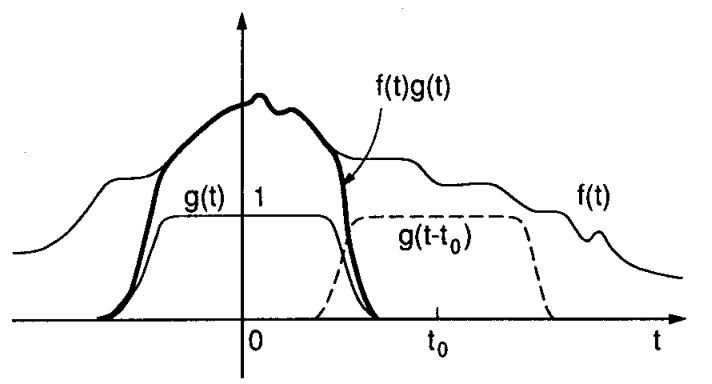
\includegraphics[width=0.5\textwidth]{Figuras/descomposicion/windowed_fourier_transform.png}
    \caption{La Transformada de Fourier de Tiempo Reducido: la función $f(t)$ es multiplicada con la función $g(t)$, obteniendo $f(t)g(t)$, repitiendo este proceso para $g(t-t_0)$, $g(t-2t_0)$ (Imagen recuperada de \cite{ten_lec_wavelets_Daubechies_1}).} 
    \label{fig:WFT}
\end{figure}

\newpage

De manera que se obtiene una descomposición temporal más detallada, se define como sigue:\\
%en deterioro de la frecuencial, pues los componentes de baja frecuencia de la onda se ven distorsionadas debido a que estas se presentan en espacios temporales amplios. 

\begin{center}

$
F(\tau, \omega) = \int_{-\infty}^{\infty} f(t) g(t - \tau) e^{-i\omega t} \, dt
$
% Fórmula obtenida de: ten_lec_wavelets_Daubechies_1
    
\end{center}


Donde \footnote{Formula recuperada de \cite{STFT}.}:

\begin{itemize}
  \item \( f(t) \) es la señal original en el dominio del tiempo.
  \item \( w(t - \tau) \) es la función de ventana que se aplica a la señal en el tiempo \( t \). Esta función de ventana suele ser una función que tiene un valor máximo en \( t \) y disminuye hacia los lados.
  \item \( e^{-i\omega t} \) es el término de frecuencia compleja.
  \item \( \omega \) es la frecuencia.
\end{itemize}

Los componentes de baja frecuencia de $f(t)$ son representados en intervalos de tiempo más grandes, por lo que el tamaño de la ventana, afecta directamente a la calidad del análisis respecto a las frecuencias que podemos rescatar: a mayor tamaño de ventana se podrá observar un mayor detalle en los componentes de baja frecuencia, caso opuesto a menor espacio de tiempo, donde las frecuencias que resulten serán más altas.

Si nos ubicamos en el plano de frecuencia contra tiempo, en el caso de la TFTR el cómo la transformación actúa es la misma para todas las locaciones pues independientemente de si tenemos una frecuencia alta o baja, el tamaño de la ventana respecto al tiempo es fijo, su relación es fija:

\begin{figure}[ht]
    \centering
    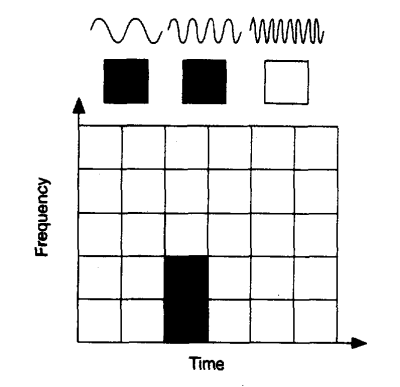
\includegraphics[width=0.5\textwidth]{Figuras/descomposicion/tiempo_frecuencia_TFTR.png}
    \caption{Plano de frecuencia contra tiempo: la manera en cómo actúa la transformación es la misma para cada ventana de tiempo, pues su tamaño es fijo e invariable para analizar cualquier frecuencia alta o baja (Recuperado de \cite{an_introduction_to_wavelets}).} 
    \label{fig:tiempo_frecuencia_TFTR}
\end{figure}

\newpage

\section{Transformada de Ondículas (WT)}

La Transformada de Ondículas o Transformada de Ondeletas (\textit{Wavelet Transform}) (WT) es una técnica avanzada en el procesamiento de señales que descompone datos o funciones en sus coeficientes de frecuencias. Depende de dos variables, la escala o frecuencia $a$ y la traslación sobre tiempo $b$, permitiendo un análisis frecuencial-temporal de la señal.

Notamos dos enfoques de Transformada de Ondículas: La Transformada Continua de Ondículas (\textit{Continuos Wavelet Transform} (CWT): 

\[
W_{f}(a, b) = \frac{1}{\sqrt{|a|}} \int_{-\infty}^{\infty} f(t) \psi^{*} \left(\frac{t-b}{a}\right) \, dt
\]

Donde:
\begin{itemize}
  \item \( f(t) \) es la función original.
  \item \( \psi^{*}(t) \) es la función conjugada compleja de \( \psi \).
  \item \( a \) y \( b \), parámetros de escala y traslación respectivamente.
\end{itemize}

Se define como la integral sobre la convolución entre nuestra señal original y una función de corta duración, que pertenece a una familia de funciones referenciadas por $a$ y $b$ que tienen la forma $\psi^{a,b}(s) = |a|^{-1/2}\psi(s-b/a)$, donde $\psi$ es llamada ondícula madre (\textit{mother wavelet}), que será nuestra función base.

Al \( \psi(t) \) comprimirse o expandirse dependiendo de $a$, $\psi^{a,0}(s)$ = $|a|^{-1/2}\psi(s/a)$ cubre diferentes rangos de frecuencia. A mayor sea el valor de $|a|$ la salida se entenderá por componentes pertenecientes a frecuencias bajas, y un valor menor de $|a|$ corresponde a frecuencias más altas. Es aquí donde surge la principal diferencia entre ésta y la TFTR, encontrando esta última una limitante en el hecho de que $g(t-\tau)$ tiene una longitud fija, lo cual acota el análisis frecuencial en cada ventana, solo $w$ puede trasladarse sobre $f(t)$ a una localización temporal adecuada:

\begin{figure}[h]
    \centering
    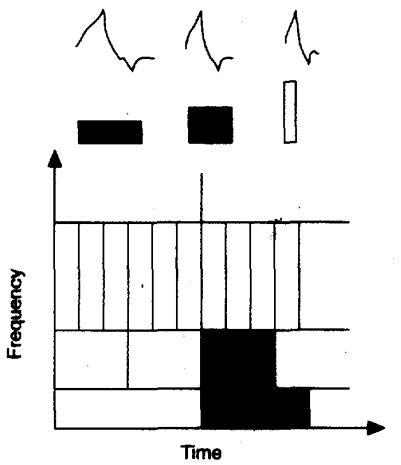
\includegraphics[width=0.5\textwidth]{Figuras/descomposicion/tiempo_frecuencia_WT.png}
    \caption{Plano de frecuencia contra tiempo: a diferencia de la TFTR, la CWT encuentra en la ampliación o compresión de $\psi^{a,b}$ la capacidad para realizar un análisis frecuencial adecuado en cada caso (Recuperado de \cite{an_introduction_to_wavelets}).} 
    \label{fig:tiempo_frecuencia_CWT}
\end{figure}

Ya que el problema que tratamos requiere el manejo de datos discretos, nos apoyaremos de la Transformada de Ondículas Discreta (\textit{Discrete Wavelet Transform}) (DWT). Se define como sigue:

\[
D_{X}(a,b) = a^{-m} \int_{-\infty}^{\infty} X(t) \psi\left( a_{0}^{-m}t-nb_{0} \right) dt
\]

Donde:
\begin{itemize}
  \item \( X(t) \) es la función original discretizada, nuestra serie de tiempo.
\end{itemize}

Típicamente, el valor de $a_0=2$ y $b_0 = 1$ para la discretización, de manera que %Donde $a=2^j$ y $b=2^jm$. 
las funciones base que son obtenidas de la ondícula madre se definen de la siguiente manera:

\[\psi_{j,k}(t) = 2^{j/2} \psi(2^{j} t - b)\]

 una familia de funciones que forman una base ortonormal para $L^2(R)$. Una de las primeras funciones $\phi$ que cumple con estos requerimientos es la función Haar, aunque en la literatura podemos encontrar otras como la función Daubechies (en la figura \ref{fig:funciones_ondículas_madre}), o la función Biortogonal.

\begin{figure}[H]
    \centering
    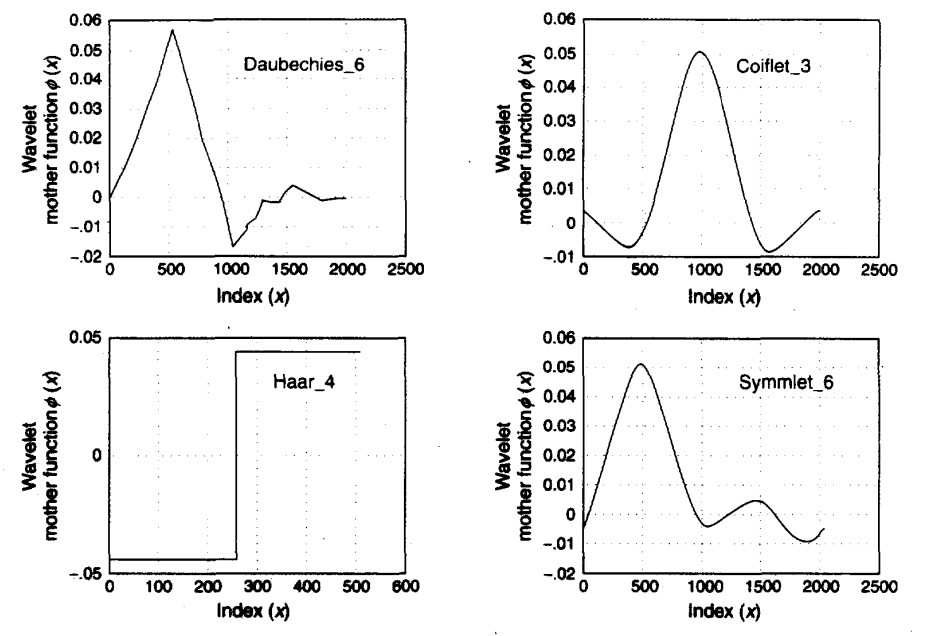
\includegraphics[width=0.5\textwidth]{Figuras/descomposicion/wavelet_mother_functions.png}
    \caption{Ejemplos de funciones de ondículas madre: Los momentos de desaparición (que se ven reflejados por el número al lado del nombre de la ondícula) se refieren a la capacidad de una ondícula para \textit{desvanecerse} al ser integrada con polinomios de cierto grado. En términos simples, si una ondícula tiene n momentos de desaparición, esto implica que el área bajo la ondícula multiplicada por un polinomio de grado n (o inferior) es igual a cero. (Recuperado de \cite{an_introduction_to_wavelets}).} 
    \label{fig:funciones_ondículas_madre}
\end{figure}

Para obtener los componente de baja y alta frecuencia de $X(t)$, la DWT usa dos conjuntos de funciones, llamadas funciones de escala (\textit{scale functions}) $\phi$ y funciones de ondícula $\psi$ (\textit{wavelet functions}) que están asociadas a un filtro de paso bajo (\textit{low-pass filter}) $\hat{g}$ y a uno de paso alto (\textit{high-pass filter}) $\hat{h}$ respectivamente. Después de filtrar los datos aplicando la transformada usando a $\psi$ y a $\phi$ como funciones base, se eliminan la mitad de los valores mediante un submuestreo, de manera que esta mitad restante caracterice las componentes bajas o altas de la señal en cada caso. Un filtro de paso bajo permite el paso de las frecuencias menores, que presentan mayor amplitud, así atenuando las características de la señal, obteniendo aquellas que representan de manera más general o suavizan a $X(t)$. Lo que obtenemos serán los coeficientes de aproximación en la resolución $2^{j}$ (\textit{Aproximation Coefficients}) ($A_{2^{j}}X$). Por otro lado, si se permite el paso de frecuencias altas o ruido presente en la señal se trata de un filtro de paso alto y se obtendrán los coeficientes de detalle en la resolución $2^{j}$ de la señal (\textit{Detail Coefficients}) ($D_{2^{j}}X$). A este procedimiento se le conoce como Codificación por Sub-bandas (\textit{Subband Coding}) \cite{wavalet_tutorial_Polizar}.

Para una descomposición superior este proceso se puede repetir, aplicando un algoritmo piramidal partiendo de los coeficientes de aproximación a un nivel de resolución $2^{j-1}$ se puede obtener los coeficientes de detalle y aproximación del nivel $2^{j}$ de manera que los coeficientes de detalle de este nivel representan las diferencias entre los coeficientes de aproximación este nivel y el anterior. Tal es el comportamiento del algoritmo de descomposición de multi-resolución propuesto por Mallat \cite{mulresolution_sigmal_desc_DWT_Mallat} como se ve reflejado en la siguiente figura:

%insertar figura del algoritmo de descomposicion de multiresolución

\begin{figure}[H]
    \centering
    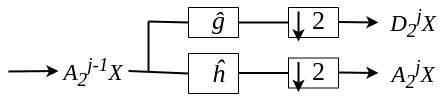
\includegraphics[width=0.5\textwidth]{Figuras/descomposicion/multiresolution_analisis_DWT.png}
    \caption{Descomposición de los componentes de aproximación $A_{2^{j-1}}X$ en sus respectivos componentes de aproximación $A_{2^{j}}X$ y de detalle $D_{2^{j}}X$, pasándolos por los filtros de paso alto y bajo $\hat{g}$ y $\hat{h}$ y aplicando un submuestreo.}
    \label{fig:algoritmo_por_subbandas}
\end{figure}

Aplicando el algoritmo de descomposición de multi-resolución a datos reales, se ve como sigue:

\begin{figure}[H]
    \centering
    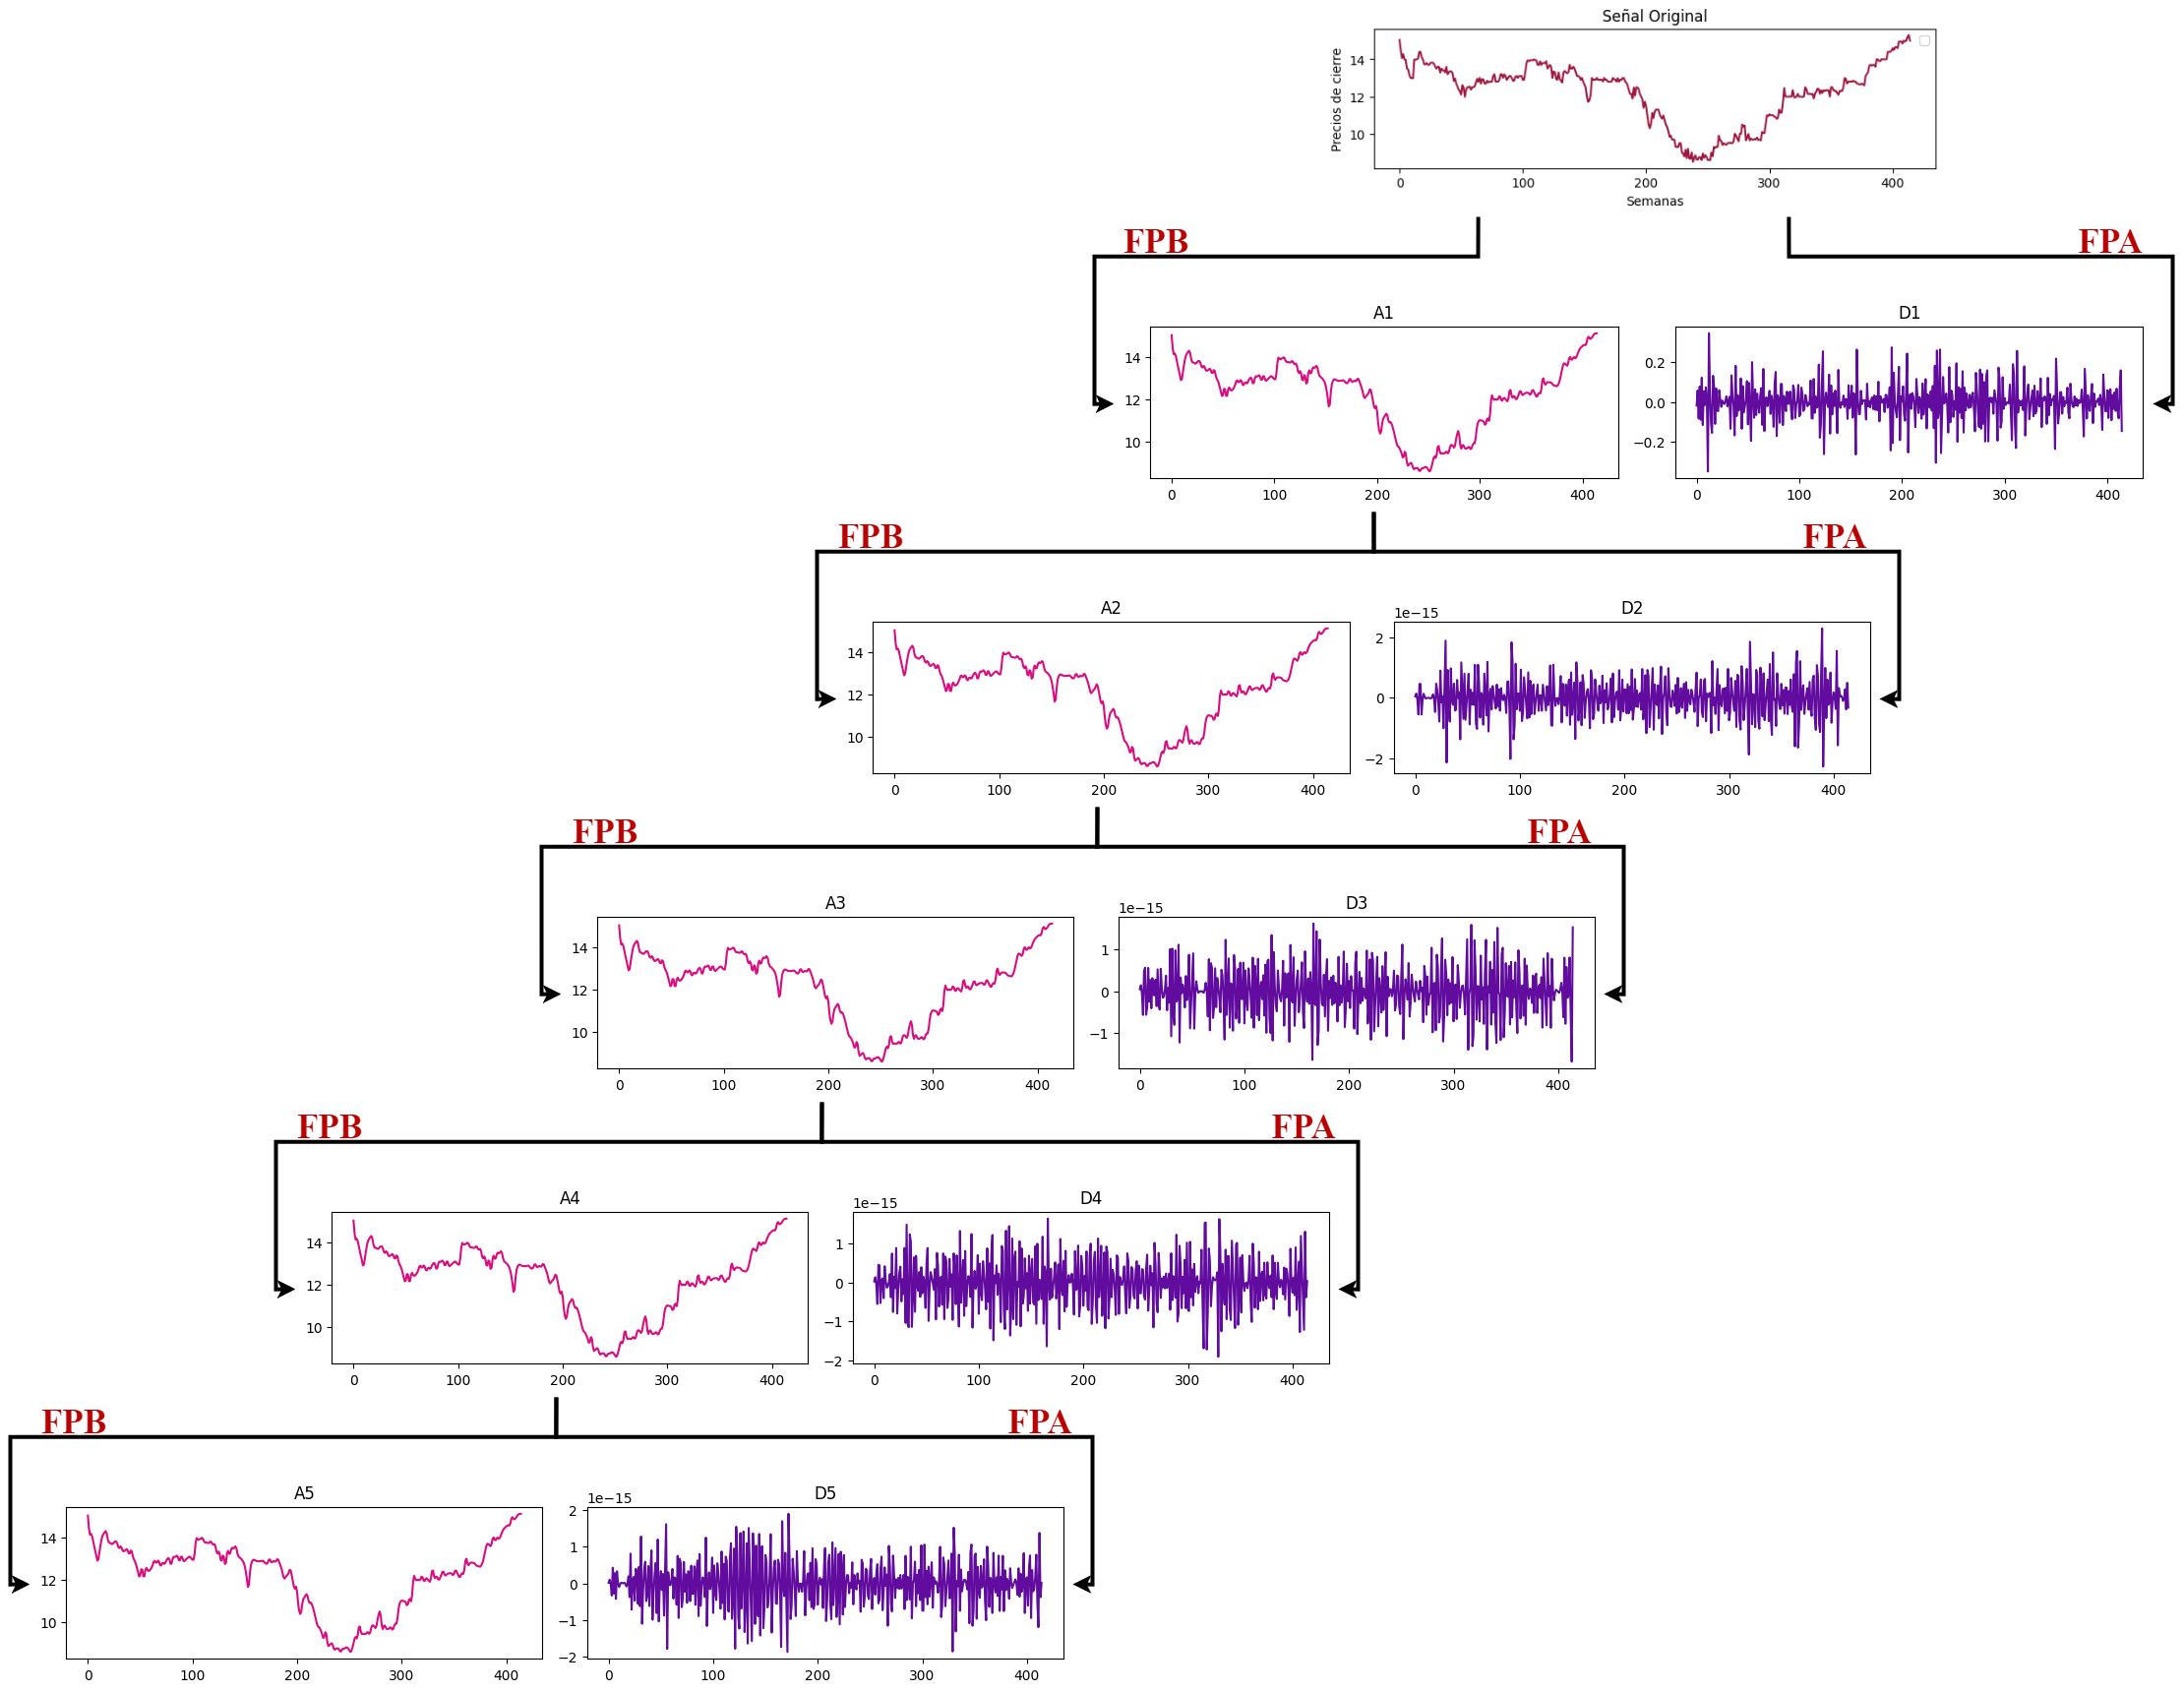
\includegraphics[width=0.9\textwidth]{Figuras/construccion_del_modelo/ACTINVRB_DWT_lvl1_5.png}
    \caption{Componentes de detalle y aproximación en cinco niveles de los datos de \textbf{ACTINVRB}.} 
    \label{fig:ACTINVRB_DWT_nivel1_5}
\end{figure}

Para la reconstrucción, las señales son aumentadas (\textit{upsampled}) por un factor de dos, pasadas por los filtros de síntesis $h[n]$ de paso bajo y $g[n]$ de paso alto y luego simplemente sumando para obtener la reconstrucción en una resolución anterior. Es a este nivel, donde trabajaremos con nuestra serie de tiempo.

\begin{figure}[H]
    \centering
    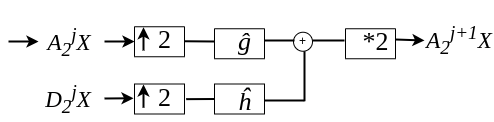
\includegraphics[width=0.5\textwidth]{Figuras/descomposicion/Recomposition_DWT.png}
    \caption{Reconstrucción de los componentes de aproximación $A_{2^{j+1}}X$ a partir de sus componentes de aproximación $A_{2^{j}}X$ y de detalle $D_{2^{j}}X$, pasándolos por los filtros de síntesis de paso alto y bajo $g$ y $h$ y aplicando un muestreo ascendente.}
    \label{fig:reconstruccion_DWT}
\end{figure}




%Desarrollo de las ondículas

 % Background Theory 

% !TEX root = ../Tesis.tex
\chapter{Redes Neuronales para análisis de series de tiempo} % Write in your own chapter title
\label{cap:RN} 

Las redes neuronales artificiales (\textit{Artificial Neural Networks}) (ANNs) se han convertido en una poderosa herramienta para resolver problemas complejos que van desde el reconocimiento de patrones hasta la toma de decisiones autónoma. Inspiradas por la configuración y el funcionamiento del cerebro humano, Nos encontramos ante un modelo computacional que consiste en un tejido de nodos interconectados entre sí. 

En el sentido de las series de tiempo, son capaces de detectar relaciones complejas y no lineales entre los datos de entrada y de salida y de aprender características y dinámicas entre y directamente de ellos \cite{Marco_TSF_Att}. A diferencia de los enfoques que usan técnicas tradicionales como el modelo autorregresivo integrado de promedio móvil (\textit{autoregressive integrated moving average}) (ARIMA) o el modelo autorregresivo integrado móvil (\textit{AutoRegressive Moving Average}) (ARMA) que se basan en suposiciones lineales o estacionales entre la información de entrada y de salida \cite{CorrOancea2014} \cite{electric_ARMA_ARIMA}, las ANNs pueden aproximar funciones no lineales. También han mostrado un mejor desempeño en comparación a modelos como la regresión lineal \cite{altay2005stock}. Aunado a esto, en la literatura podemos encontrar algunos otros modelos como el caso de las maquinas de soporte vectorial (\textit{Support Vector Machines}) (SVMs) \cite{YANG202218_SVM1} \cite{parray2020time}, árboles de desición \cite{arboles1} y bosques aleatorios \cite{khan2020predicting_randomforest22} \cite{randomforest1} que han mostrado un desempeño igualmente favorable. Para fines de este proyecto, veremos si las diferentes arquitecturas de ANNs en conjunto de la DWT generará resultados igual o mejor logrados.

%Estos se organizan en capas, dentro de las cuales cada neurona recibe datos como entrada y, junto con cierta ponderación de estos a partir de pesos y sesgos, lleva a cabo una combinación lineal y aplica una función de activación a dicho resultado para generar una salida o impulso. En un sentido general, el número de capas con el que cuenta una red es indistinto, pero siempre se puede identificar una capa de entrada, que es aquella por donde son consumidos los datos, una de salida, de donde se obtiene el resultado del procesamiento en la red y un número arbitrario de capas ocultas. 



\section{Redes Neuronales Artificiales}
Como se mencionó arriba, son un modelo de procesamiento masivo y paralelo, compuesto de neuronas conectadas entre sí con la capacidad de almacenar 'experiencia' a través del aprendizaje. A continuación se profundizará más sobre esto último. 

La unidad básica de una red neuronal es el perceptron: un combinador lineal que recibe varias entradas númericas en conjunto con un valor inmutable llamado sesgo, que pondera con cierto peso y las suma. Todo esto seguido por una función de activación que genera una respuesta o estimulo para las unidades en las siguientes capas.

\[
y = f\left(\sum_{i=1}^{n} w_i x_i + b\right)
\]

Donde:
\begin{itemize}
    \item $x_i$ es entrada $i$-ésima de la neurona.
    \item $w_i$ es el peso asociado a la entrada $x_i$ de la neurona.
    \item $b$ es el sesgo de la neurona.
    \item $f$ es una función de activación no lineal diferenciable.
\end{itemize}

La estructura de una red neuronal comprende una capa de entrada, una o más capas ocultas y una capa de salida. En cada una de ellas se encuentran cierto número de neuronas conectadas con las de la capa anterior y siguiente. Estas se comunican 'propagando hacia adelante' la información que se recibe hasta generar una respuesta por parte del modelo. Esto ocurre mediante las entradas de las unidades en capas sucesivas que reciben los impulsos de las anteriores. 

El peso ligado a cada una de las entradas de cada neurona regula qué tan importante es dicha entrada para esta, a menor peso, dicha entrada se involucrará menos en el computo de una respuesta y lo mismo en caso contrario. Así, al regular estos parámetros podemos controlar qué respuesta se genera el modelo al ser 'alimentado' por alguna entrada. Esto es especialmente conveniente para que una red nos sea útil, de esta manera se construye el aprendizaje de la red hasta obtener un modelo que cumpla la tarea para el cual fue creado. Para esto existe la etapa de entrenamiento. Durante este proceso los pesos de las conexiones entre nodos y sus sesgos se ajustan utilizando algoritmos de optimización.

\section{Entrenamiento de una Red Neuronal}

La capacidad de predicción en una red neuronal esta ligada fuertemente a qué ha aprendido de los datos, esto sucede gracias al entrenamiento empleado en esta. Este procedimiento se compone de dos partes fundamentales: el paso de propagación hacia adelante (\textit{feedforward}) y el paso de retro-propagación (\textit{backpropagation}).

El primer paso, \textbf{propagación hacia adelante}, se encarga de evaluar la señal $x_t$ en la red, siendo propagada a través de esta, capa por capa. Cada neurona calcula la suma ponderada y pasa la respuesta a la función de activación correspondiente, esta es la entrada para las neuronas de la siguiente capa. 

Cuando la propagación termina, la salida generada por la red a partir de esa entrada, llamémosle $\hat{y}_t$, se compara con el valor que esperábamos con dicha entrada, digamos $y_t$. Esro sucede a partir de la función de error $E$, que nos permite medir qué tan cerca se encuentra la predicción del valor real y así evaluar el desempeño actual de la red. Podemos encontrar funciones de error como el Error Cuadrático Medio (\textit{Mean Square Error}) (MSE), que emplearemos más adelante o el Error Absoluto Medio (\textit{Mean Absolute Error}) (MAE):
%Entropía Cruzada (\textit{Cross-Entropy})

\[ \text{MSE} = \frac{1}{n} \sum_{i=1}^{n} (y_i - \hat{y}_i)^2
\]

\[\text{MAE} = \frac{1}{n} \sum_{i=1}^{n} |y_i - \hat{y}_i|\]

%\[ \text{Entropía Cruzada} = -\sum_{i=1}^{n} y_i \log(\hat{y}_i)\]

Conociendo el error, es cuando la \textbf{retro-propagación} actúa. Se encarga de calcular los gradientes de $E$ respecto a los parámetros de la red (pesos y sesgos de todas las unidades que la componen). Para ello hacemos uso de la regla de la cadena (\textit{chain rule}) \cite{understanding_backpropagation_Kostadinov}. Sea $w_{i,j}^{c}$ un solo peso de conexión entre las neuronas $i, j$ de las capas $c-1$ oculta y $c$ de salida respectivamente, $b_{j}^{c}$ el sesgo de $j$, $a_i^{c-1}$ es la salida de la función de activación de la capa anterior y $f_j(z^c_j)$ es la señal de $j$ \footnote{Nótese que $f_j(z^c_j)$ se puede ver como $a_j^{c}$} como se puede ver en la Figura~\ref{fig:Feed-forward}.

\begin{figure}[H]
    \centering
    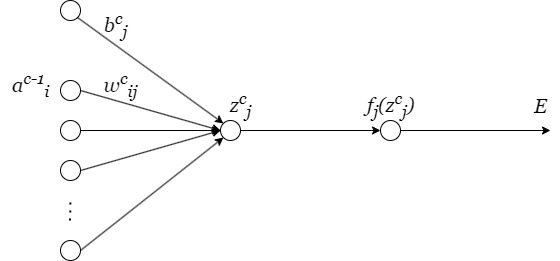
\includegraphics[width=0.8\textwidth]{Figuras/redes_neuronales/Forward_neurona.jpg}
    \caption{Esquema de la propagación hacia adelante en una neurona de salida} 
    \label{fig:Feed-forward}
\end{figure}

Se tiene entonces que los gradientes de $E$ respecto a los parámetros de la neurona son \footnote{Según las derivaciones mostradas por Haykin, S. y por Hertz, J.A., Palmer, R.G., Krogh, A. \cite{haykin2008neural} \cite{hertz1991introduction}}:

\begin{center}
    $\dfrac{\partial E}{\partial w_{i,j}^{c}} = \dfrac{\partial E}{\partial z_{j}^{c}}a_i^{c-1}$
\end{center}

Y también respecto a algún sesgo en $c$:

\begin{center}
    $\dfrac{\partial E}{\partial b^c_j} = \dfrac{\partial E}{\partial z_{j}^{c}}$
\end{center}

Donde el termino de gradiente local en neuronas de capas de salida:

\begin{center}
    $\dfrac{\partial E}{\partial z_{j}^{c}} = E f'(z^c_j)$
\end{center}

Debido a que las neuronas de capas ocultas no cuentan con una salida esperada, esta debe de ser determinada recursivamente en términos de las salidas esperadas de las unidades en las capas sucesivas. De esta forma es en la que el cálculo del gradiente se efectúa para estas, dependiendo de los gradientes de las neuronas a las cuales esta se conecta y a su vez, el obtener el gradiente de unidades en capas anteriores es mediante el gradiente calculado de esta última neurona. Es así que la retro-propagación de los gradientes de los parámetros de la red actúa.

Sea entonces $c$ una capa oculta y $c+1$ es la capa de salida y $k$ es una neurona a elegir en el conjunto de las unidades para las cuales $j$ tiene una salida:

\begin{figure}[H]
    \centering
    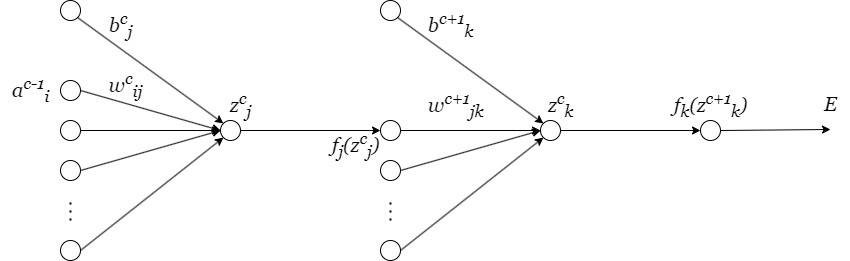
\includegraphics[width=0.8\textwidth]{Figuras/redes_neuronales/Feed-forward 2 neuronas.jpg}
    \caption{Esquema de la propagación hacia adelante en una neurona en una capa oculta conectada a una neurona de salida} 
    \label{fig:Feed-forward2}
\end{figure}

Así, el gradiente local de $j$:

\[
\dfrac{\partial E}{\partial z_{j}^{c}} = f'(z^c_j)\sum_{k} \dfrac{\partial E}{\partial z_{k}^{c+1}} w^{c+1}_{jk}
\]

Con los gradientes calculados, el algoritmo de optimización aplica una estrategia para ajustar los pesos de las conexiones en la red y los sesgos de cada neurona para minimizar la diferencia entre la salida que obtuvimos de esta y los valores originales. Algunos ejemplos de algoritmos de optimización más comúnmente usados son Descenso por el Gradiente (\textit{Gradient Descent}) (GD), Descenso por el Gradiente Estocástico (\textit{Stochastic Gradient Descent}) (SGD), Estimación Adaptativa de Momento (\textit{Adaptative Moment Estimation}) (ADAM) y Levenberg-Marquardt (LM). A continuación profundizaremos sobre estos. 

\subsection{Algoritmos de Optimización}

\begin{itemize}
    \item \textbf{Descenso por el gradiente}
    Es el método más común para minimizar $E$. Ajusta los pesos y sesgos en la dirección opuesta al gradiente multiplicado por la tasa de aprendizaje (\textit{learning rate}) (debido a que el gradiente indica la dirección hacia donde crece la función o donde se encuentra un máximo local).
    Este proceso se repite iterativamente durante varias épocas \footnote{Una época comprende una iteración del proceso completo de entrenamiento, es decir propagación hacia adelante, cálculo en $E$, retro-propagación y algoritmo de optimización.}, hasta que la función de pérdida converge o se detiene según algún criterio predefinido.

    Así entonces, las actualizaciones de cada peso y sesgo está dado por:

\begin{center}
    $w_{ij}^{c} := w_{ij}^{c} - \alpha \dfrac{\partial E}{\partial z_{j}^{(c)}}a_i^{c-1}$

    $b^c_j := b^c_j - \alpha \dfrac{\partial E}{\partial z_{j}^{(c)}}$
\end{center}

    \item \textbf{SGD}
    Es una variante específica del Descenso por el Gradiente.
    En vez de calcular el gradiente utilizando todo el conjunto de datos de entrenamiento, se obtiene utilizando solo un subconjunto de los datos (mini lotes\footnote{\textit{mini batch}}) seleccionado de manera aleatoria en cada iteración del entrenamiento ayudando a evitar mínimos locales y puntos de estancamiento durante el entrenamiento. Esto hace que el cálculo del gradiente sea más eficiente, especialmente para conjuntos de datos grandes.
    
    \item \textbf{ADAM}
    Es un optimizador que combina la idea del descenso por el gradiente con el movimiento promedio de los momentos. Utiliza estimaciones adaptativas del primer y segundo momento de los gradientes para ajustar la tasa de aprendizaje de forma individual para cada parámetro de la red, lo que lo hace especialmente útil en problemas con características de datos variables o no estacionarias. \cite{adam_kingma}
    Además esto permite que, durante la optimización de la función de error ADAM da 'pasos' conforme al comportamiento del gradiente en ese instante, alcanzando el mínimo de manera más precisa. 

    ADAM emplea dos arreglos del tamaño de los parámetros de la red que se encargarán de contener el movimiento promedio o media móvil del primer y segundo momento de los gradientes, estos son actualizados en cada iteración del algoritmo ponderando los gradientes y el cuadrado de este respectivamente junto con $m_{t-1}$ y $v_{t-1}$, los vectores de la corrida anterior (linea 4 y 5). Finalmente se actualizan los parámetros $x_t$ (linea 7) con los vectores cuando se encuentran corregidos a partir de la taza de decaimiento (linea 6), esto para evitar un sesgo en la inicialización en cero.
    
    . %También incluye un término de momentum que ayuda a acelerar la convergencia y suaviza las actualizaciones de los pesos.

    \begin{algorithm}[H]
        \caption{Algoritmo de Optimización ADAM}
        \KwIn{Conjunto de datos $X$, tasa de aprendizaje $\alpha$, $\beta_1$, $\beta_2$, $\epsilon$}
        \SetAlgoLined
        \SetKwComment{Comment}{\% }{}
        \SetKwInOut{Input}{Entrada}
        \SetKwInOut{Output}{Salida}
        \Input{Parámetros del modelo: $x_0$}
        \Input{Momentos de primer y segundo orden: $m_0 = 0$, $v_0 = 0$}
        \Input{Contador de iteraciones: $t = 0$}
        \BlankLine
        \While{no se alcance el criterio de parada}{
            $t \gets t + 1$\;
            Calcular el gradiente: $g_t = \nabla_x E(x_{t-1})$\;
            Actualizar el momento de primer orden: $m_t = \beta_1 m_{t-1} + (1 - \beta_1) g_t$\;
            Actualizar el momento de segundo orden: $v_t = \beta_2 v_{t-1} + (1 - \beta_2) g_t^2$\;
            Corregir los momentos de primer y segundo orden: $\hat{m}_t = \frac{m_t}{1 - \beta_1^t}$, $\hat{v}_t = \frac{v_t}{1 - \beta_2^t}$\;
            Actualizar los parámetros: $x_t = x_{t-1} - \alpha \frac{\hat{m}_t}{\sqrt{\hat{v}_t} + \epsilon}$\;
        }
        \Output{Parámetros del modelo $x_t$}
    \end{algorithm}
    
    \item \textbf{Levenberg Marquardt (LM)}
    Es un algoritmo de optimización no lineal utilizado principalmente en problemas de ajuste de curvas y regresión no lineal. A diferencia de los métodos basados únicamente en el gradiente, LM utiliza una estrategia de optimización iterativa que combina técnicas de descenso por el gradiente y gauss-newton. El algoritmo ajusta los parámetros de manera iterativa, utilizando una matriz de aproximación o la misma matriz hessiana en combinación con el gradiente para guiar la búsqueda hacia el mínimo local de la función de error.
    La dirección de búsqueda del algoritmo se define como sigue:

    \begin{center}
    $\Delta x = -[H + \lambda I] ^{-1} \nabla E(x)$
    \end{center}

    Donde:
    \begin{itemize}
        \item $x$ son los parámetros de la red.
        \item $E(x)$ es la función de error.
        \item $H$ es la matriz Hesiana de $E(x)$.
    \end{itemize}

    \begin{algorithm}
        \caption{Algoritmo de Levenberg-Marquardt}
        \KwData{Función de error $E(x)$, punto inicial $x_0$, parámetros de ajuste $\lambda_0$, tolerancia $\epsilon$}
        \KwResult{Solución $\mathbf{x}^*$}
        Inicializar $x \leftarrow x_0$\;
        Inicializar $\lambda \leftarrow \lambda_0$\;
        Definir $\epsilon_1 \leftarrow$ Tolerancia para la convergencia del método\;
        Definir $\epsilon_2 \leftarrow$ Tolerancia para el valor del gradiente\;
        \Repeat{convergencia}{
            Calcular el vector de gradiente $\nabla E(x)$\;
            Calcular la matriz Hessiana $H$\;
            Calcular el paso de Levenberg-Marquardt: $\Delta \mathbf{x} = -[H + \lambda I]^{-1} \nabla E(x)$\;
            Calcular el valor de la función de error con el paso propuesto: $f_{\text{prop}} = f(\mathbf{x} + \Delta \mathbf{x})$\;
            Calcular el valor de la función de error en el punto actual: $f_{\text{actual}} = f(\mathbf{x})$\;
            \If{$f_{\text{prop}} < f_{\text{actual}}$}{
                Aceptar el paso: $\mathbf{x} \leftarrow \mathbf{x} + \Delta \mathbf{x}$\;
                Actualizar $\lambda$: $\lambda \leftarrow \frac{\lambda}{2}$\;
            }
            \Else{
                Rechazar el paso: No actualizar $\mathbf{x}$\;
                Aumentar $\lambda$: $\lambda \leftarrow 2\lambda$\;
            }
            \If{$|$ $f_{\text{prop}} - f_{\text{actual}}$ $|$ $> \epsilon_1$ o $|| \nabla E(x)|| > \epsilon_2$}{
                Detener el algoritmo\;
            }
        }
        \end{algorithm}

    
\end{itemize}

    A pesar de ser un método efectivo, LM no es un algoritmo tan usado como SGD o ADAM debido a que es computacionalmente costoso, debido al calculo de la matriz hessiana o su aproximación. 
    

\newpage

\section{Redes Neuronales Auto-regresivas}

Las ARNNs, o redes neuronales auto-regresivas (\textit{Autorregresive Neural Networks} también llamadas NARNN (por \textit{Not linear Autorregresive Neural Networks}), se emplean en el estudio de series temporales y en tareas de predicción secuencial. Se trata de un tipo específico de arquitectura de redes neuronales que consiste en predecir los valores futuros a partir de los pasados $d$ valores, contemplando la idea de que el comportamiento en el pasado de una serie temporal tiene impacto en su desempeño en el futuro. Buscan estimar $p(x_{t} | x_{t-1}, ..., x_1)$

Dada una serie temporal $\{ x_1, x_2, \ldots, x_t \}$, donde $x_i$ representa una muestra en el tiempo $i$, una ARN puede predecir el valor futuro $\hat{x}_{t+1}$ basado en las observaciones pasadas $x_{t-1}, x_{t-2}, \ldots, x_{t-d}$, con $t,d \in \mathbb{N} $ 

Una ARN puede expresarse como una función $f$ que mapea las observaciones pasadas a la predicción futura:

\[
\hat{x}_{t} = f(x_{t-1}, x_{t-2}, \ldots, x_{t-d})
\]

En la práctica, las ARN suelen tener una estructura recurrente \footnote{Según Haykin, podemos interpretar a una ARN como una Red Neuronal Recurrente en si misma, sin embargo para fines de este trabajo, trataremos a ambas como entidades independientes.} (que trataremos más adelante), hecho que no implica el desuso de arquitecturas básicas con propagación hacia adelante (\textit{feedforward}) como unidad base. 

\begin{figure}[h]
    \centering
    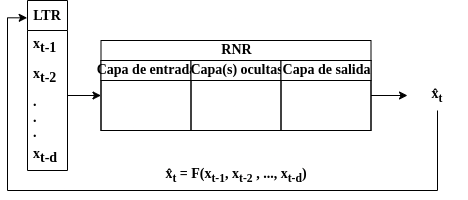
\includegraphics[width=0.5\textwidth]{Figuras/redes_neuronales/NARNN_diagrama.png}
    \caption{Esquema general de una RNN} 
    \label{fig:rRNN_diagrama}
\end{figure}

Sin embargo, implementar capas recurrentes permite que la red capture dependencias o relaciones implícitas a lo largo de la serie temporal y realice predicciones aun más precisas (como también veremos más adelante). Las ARN también pueden incorporar capas convolucionales o capas completamente conectadas, dependiendo de la naturaleza de los datos y la complejidad del problema de predicción. 

\section{Redes Neuronales Recurrentes}

Las Redes Neuronales Recurrentes (\textit{Recurrent Neural Networks}) (RNNs) son un sistema dinámico no lineal. A diferencia de las redes neuronales tradicionales, las RNN tienen conexiones retro-alimentadas, lo que significa que las salidas de algunos de sus nodos se incluyan como parte de la entrada de los mismos en siguientes iteraciones del proceso de predicción y la información que fluye a través de éstas pueda hacerlo cíclicamente. Esto permite retener y aprovechar información sobre estados anteriores a lo largo de la secuencia de datos (persistencia). Están diseñadas para modelar datos secuenciales, como palabras en un texto o muestras en una serie temporal cuyos datos en cierto espacio de tiempo $\delta t$ guardan relación con algún intervalo $\delta (t-d)$ en el pasado. 

Dada una secuencia de entrada $\{ x_1, x_2, \ldots, x_t \}$%, y una secuencia de salida correspondiente $\{ y_1, y_2, \ldots, y_t \}$, 
una RNN se define de forma general como sigue:

\[ h_t = f(W \cdot [x_t, h_{t-1}] + b) \]
\[ o_t = g(h_t) \]

Donde:
\begin{itemize}
    \item $h_t$ es el estado oculto o estado interno en el tiempo $t$. Representa la memoria de la red en ese momento y se calcula utilizando una función de activación $f$ que toma como entrada el elemento actual $x_t$ y el estado oculto anterior $h_{t-1}$.
    \item $o_t$ es la salida de la red en el tiempo $t$, calculada utilizando una función de activación $g$ aplicada al estado oculto $h_t$ \footnote{También se suele ver a $g=f$ de manera que $o_t = h_t$.}.
    \item $f$ y $g$ son funciones de activación no lineales, como la función sigmoide ($\sigma$) o la función tangente hiperbólica ($tanh$), que introducen la no linealidad en el modelo y permiten a la red capturar relaciones complejas en los datos secuenciales.
\end{itemize}

Una de las arquitecturas más simples de las RNNs son los Perceptrones Multicapa Recurrentes (\textit{Recurrent Multilayer Perceptron}) RMLP que se caracteriza porque las neuronas de cada una de sus capas recibe como parte de su entrada el valor de salida que esta misma genero en la iteración anterior, es decir, a salida de una capa en un tiempo $t$ puede ser una función de su salida en el tiempo $t-1$, además de la entrada actual. Se define como sigue:

\[x_{I,n+1} = \Psi_I(x_{I,n},U_{n})\]
\[x_{II,n+1} = \Psi_{II}(x_{II,n},x_{I,n+1})\]
\begin{center}
.\\
.\\
.\\  
\end{center}

\[x_{o,n+1} = \Psi_o(x_{o,n},x_{M,n+1})\]

A pesar de que las RNNs hacen uso de información en el pasado para modelar el comportamiento actual, la manera cíclica de actuar de éstas sólo influye cuando los datos que necesitamos pertenecen al pasado inmediato anterior de la predicción actual. Si por el contrario, lo que intentamos predecir está ligado a muestras que se presentaron con mayor anterioridad, la red perderá su capacidad de predicción con base a esta información. Es aquí donde se nos presenta el llamado problema de Dependencias a Largo Plazo  (\textit{Long-term dependencies}) \cite{understanding_lstm_Olah}. 

\subsection{Retro-propagación a través del tiempo}

Se trata de una extensión del algoritmo de retro-propagación util para el ajuste de parámetros en una red recurrente.

En principio, se usa la técnica de desdoblamiento que menciona Haykin, S.: \cite{haykin2008neural} el modelo recurrente representa sus múltiples pasos en el tiempo a través de una red neuronal de propagación hacia adelante:

\begin{enumerate}
    \item Para cada paso temporal en $(t_0,t]$ la red de propagación hacia adelante, llamémosle $F$, tiene una capa con N neuronas, que es el número total de unidades en la red recurrente $R$.

    \item Para cada paso temporal, existe una conexión de la neurona $i$ de la capa $c$ a la neurona $j$ en la capa $c+1$ 
\end{enumerate}

El conjunto de datos que se usará para entrenamiento se particionará en intervalos temporales llamados épocas. Sea $t_0$ y $t_1$ el tiempo de inicio y fin de cierta época. La función de error total de la salida de la red:

\[
E_{total} = \sum^{t_1}_{n=n_0}\sum_{i}E_{i,t}
\]

Donde:
\begin{itemize}
    \item $i$ es el conjunto de neuronas de la red
    \item $E_{i,t}$ es el error de la salida esperada de $i$
\end{itemize}

Así, el algoritmo de retro-propagación a través del tiempo se define como sigue:

\begin{enumerate}
    \item Se realiza el paso de la propagación hacia adelante y se asegura el estado de la red (se guardan sus parámetros).
    \item Se realiza el paso de la retro-propagación:

    \[
    \dfrac{\partial E_{total}}{\partial v_{i,t}} = \left\{
    \begin{array}{ll}
    \varphi'(v_{i,t})E_{i,t} & \text{si } t > t_1 \\
    \varphi'(v_{i,t}) \left[E_{i,t}+\sum_{j}w_{ij}\dfrac{\partial E_{total}}{\partial v_{j,t+1}}\right] & \text{si } t_0 < t < t_1
\end{array}
\right.
    \]
    
    Donde:
    \begin{itemize}
        \item $\varphi'(\cdot)$ es la derivada de la función de activación.
        \item $v_{i,t}$ es el estado de la neurona $i$ en el tiempo $t$
    \end{itemize}

    Así las iteraciones sobre la formula actúan desde el tiempo $t_1$ hasta $t_0$.
    
    \item Una vez concluida la retro-propagación, se realiza el ajuste de pesos correspondiente, según el algoritmo de optimización elegido. 

    \[
    w_{ij} := w_{ij} - \alpha \dfrac{\partial E_{total}}{\partial w_{ij}}
    \]

    Y:
    \[
    \dfrac{\partial E_{total}}{\partial w_{ij}} = -\sum^{t_1}_{t=t_0+1}\dfrac{\partial E_{total}}{\partial v_{i,t}}x_{j,t-1}
    \]

    Donde:
    \begin{itemize}
        \item $x_{j,t-1}$ es la entrada aplicada a la $j$-ésima conexión de la neurona $i$ en el tiempo $t-1$.
    \end{itemize}
    
\end{enumerate}

\subsection{Redes Neuronales LSTM}

Las redes neuronales con células de Memoria de Corto y Largo Plazo o LSTM (\textit{Long Short-Term Memory}) son un tipo especializado de RNNs, presentadas por primera vez por Hochreiter y Schmidhube (1991) \cite{LSTM}, diseñadas para manejar con mayor eficacia los problemas de dependencias entre datos secuenciales. Las LSTM tienen unidades de memoria llamadas ''células de memoria'' que les permiten retener y actualizar información durante largos períodos, a diferencia de las RNNs comunes.

La idea central de una célula LSTM es su estado(\textit{cell state}) y sus diferentes compuertas. La primera actúa como una banda transportadora o autopista que transfiere información a lo largo de la cadena de secuencia de la célula, mientras que las compuertas actúan como redes neuronales con la capacidad de aprender qué información se olvidará o recordará en iteraciones siguientes.  Dada una secuencia de entrada $\{ x_1, x_2, \ldots, x_t \}$ y una secuencia de salida correspondiente $\{ y_1, y_2, \ldots, y_t \}$, una célula de memoria LSTM realiza la siguiente operación:

\[ i_t = \sigma(W_{i} \cdot [x_t, h_{t-1}] + b_i) \]
\[ f_t = \sigma(W_{f} \cdot [x_t, h_{t-1}] + b_f) \]
\[ g_t = \tanh(W_{g} \cdot [x_t, h_{t-1}] + b_g) \]
\[ C_t = f_t \odot C_{t-1} + i_t \odot g_t \]
\[ o_t = \sigma(W_{o} \cdot [x_t, h_{t-1}] + b_o) \]
\[ h_t = o_t \odot tanh(C_t) \]

Donde:
\begin{itemize}
    \item $i_t$, compuerta de entrada (\textit{input gate}): determina qué valores serán los candidatos para formar parte del nuevo estado de la célula $C_t$.
    \item $f_t$, compuerta de olvido (\textit{forget gate}): mediante la función sigmoide se decide que datos olvidar (0) o mantener (1) del estado oculto (\textit{hidden state}) anterior $h_{t-1}$.
    \item $g_t$ es la candidata de celda.
    \item $C_t$ es el estado de la célula en el tiempo $t$, que almacena y actualiza la información relevante a largo plazo. Se obtiene al multiplicar $g_t$ por $f_t$ obteniendo los valores candidatos omitiendo aquellos que se decidieron olvidar, al sumar $i_t \cdot g_t$ tenemos todas las actualizaciones de los valores de $C_t$.
    \item $o_t$ compuerta de salida (\textit{output gate}).
    \item $h_t$ es el estado oculto en el tiempo $t$, que se calcula utilizando una versión filtrada del estado de la célula.
\end{itemize}

\begin{figure}[h]
    \centering
    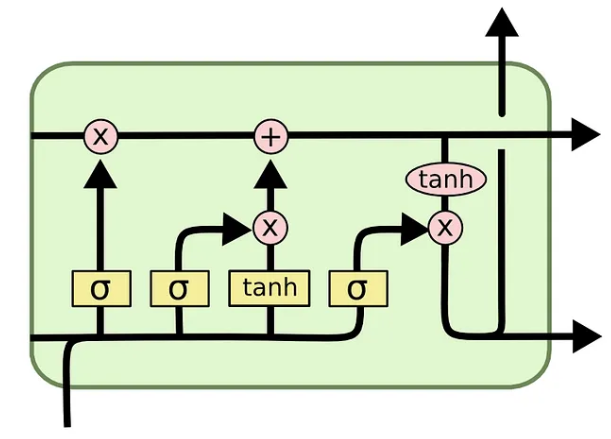
\includegraphics[width=0.5\textwidth]{Figuras/redes_neuronales/diagrama_celda_LSTM.png}
    \caption{Esquema general de una célula LSTM (Recuperado de \cite{understanding_lstm_Olah}).} 
    \label{fig:diagrama_LSTM}
\end{figure}

%Aunado al hecho que las redes neuronales con células LSTM resulven el problema de las Dependencias de Termino largo, esta arquitectura fue ideada para solventar el problema del gradiente desvaneciente (\textit{Vanishing Gradient}). El problema del gradiente desvaneciente es una limitación que puede surgir durante el entrenamiento de redes neuronales profundas, especialmente aquellas con muchas capas. Se manifiesta cuando los gradientes calculados durante el proceso de retropropagación disminuyen exponencialmente a medida que se propagan hacia atrás a través de las capas de la red. Se vuelve problemático porque los pesos de las capas iniciales de la red apenas se actualizan durante el entrenamiento, lo que significa que estas capas aprenden muy lentamente o incluso no aprenden en absoluto. Como resultado, las capas posteriores de la red pueden recibir poca o ninguna información útil de las capas anteriores, lo que dificulta el aprendizaje efectivo de la red en su conjunto.

\subsubsection{Entrenamiento de una red LSTM}

El entrenamiento de una red con células LSTM parte del mismo principio que el de un perceptrón multicapa: un paso de propagación hacia adelante, evaluación del error por medio de la función $E$, la retro-propagación con el cálculo de sus respectivos gradientes y la optimización según el algoritmo que se aplique.

Para obtener los gradientes de $E$ con respecto de cada uno de los componentes con ayuda de la regla de la cadena. Por ejemplo, se sabe que durante la propagación hacia adelante el flujo de la información de $o_t$:

\begin{center}
    $o_t$ a $E$: $o_t \longrightarrow h_t \longrightarrow E$
\end{center}
Por lo que el cálculo del respectivo gradiente es:

$\dfrac{E}{o_t} = \dfrac{\partial E}{\partial h_t} \cdot \tanh(c_t)$

Y para $a_o = W_{o} \cdot [x_t, h_{t-1}] + b_o$:

\begin{center}
    $a_o$ a $E$: $a_t \longrightarrow o_t \longrightarrow h_t \longrightarrow E$
\end{center}

Y entonces:

$\dfrac{E}{\partial a_o} = \dfrac{\partial E}{\partial h_t} \cdot \tanh(c_t) \cdot o_t(1-o_t)$ \footnote{El desarrollo de los anteriores se puede ver reflejado en \ref{ApA}.}

Y consecuentemente para los demás compuertas de la célula \cite{LSTM_gradients_Rahuljha} \footnote{Aquí podemos encontrar la derivación completa de cada una de las compuertas.} \cite{LSTM_fbp_calc_grad_Mallya}

Los gradientes de la célula LSTM:

\begin{center}
    $\dfrac{\partial E}{h_t} = y_t - h_t$ \footnote{Solo si se usa a $E = ECM(y_t,h_t)$.}
    
    $\dfrac{\partial E}{\partial o_t} = \dfrac{\partial E}{\partial h_t} \cdot tanh(C_t)$

    $\dfrac{E}{\partial a_o} = \dfrac{\partial E}{\partial h_t} \cdot \tanh(c_t) \cdot o_t(1-o_t)$ 

    $\dfrac{\partial E}{\partial C_t} = \dfrac{\partial E}{\partial h_t} \cdot o_t \cdot (1-tanh^2(C_t))$

    $\dfrac{\partial E}{\partial g_t} = \dfrac{\partial E}{\partial C_t} \cdot i_t$

    $\dfrac{E}{\partial a_C} = \dfrac{\partial E}{\partial C_t} \cdot i_t \cdot (1-g_t^2)$ 

    $\dfrac{\partial E}{\partial i_t} = \dfrac{\partial E}{\partial C_t} \cdot g_t$

    $\dfrac{E}{\partial a_i} = \dfrac{\partial E}{\partial C_t} \cdot g_t \cdot i_t(1-i_t)$ 

    $\dfrac{\partial E}{\partial f_t} = \dfrac{\partial E}{\partial C_t} \cdot C_{t-1}$

    $\dfrac{E}{\partial a_f} = \dfrac{\partial E}{\partial C_t} \cdot C_{t-1} \cdot f_t(1-f_t)$ 

    $\dfrac{E}{\partial C_{t-1}} = \dfrac{\partial E}{\partial C_t} \cdot f_t$ 
\end{center}

Definimos $Z_t = [x_t, h_{t-1}]$. Durante la propagación hacia adelante $Z_t$ tiene flujo por medio de las compuertas de entrada, salida, de olvido y el estado de la célula:

\begin{center}
    $\dfrac{\partial E}{\partial Z_t} = W_f^T\dfrac{\partial E}{\partial a_f} + W_i^T\dfrac{\partial E}{\partial a_i} + W_o^T\dfrac{\partial E}{\partial a_o} + W_C^T\dfrac{\partial E}{\partial a_C}$
\end{center}

Por último, para los pesos y sesgos:

\begin{center}
    $\dfrac{\partial E}{W_t} = \dfrac{\partial E}{\partial a_f} \cdot z_t^T$, 
    $\dfrac{\partial E}{b_t} = \dfrac{\partial E}{\partial a_f}$

    $\dfrac{\partial E}{W_i} = \dfrac{\partial E}{\partial a_i} \cdot z_t^T$, 
    $\dfrac{\partial E}{b_i} = \dfrac{\partial E}{\partial a_i}$

    $\dfrac{\partial E}{W_o} = \dfrac{\partial E}{\partial a_o} \cdot z_t^T$, 
    $\dfrac{\partial E}{b_o} = \dfrac{\partial E}{\partial a_o}$
\end{center}

\subsection{Redes Neuronales GRU}

Las redes neuronales con Unidades Recurrentes Cerradas (\textit{Gated Recurrent Unis}) o GRU, propuestas por Cho, et. al \cite{GRU}, son una arquitectura de RNR diseñada para modelar y procesar eficientemente datos secuenciales. Las GRU, al igual que las LSTM, tienen como objetivo resolver el problema de las dependencias a largo plazo en datos secuenciales. No obstante, las GRU resultan más sencillas que las LSTM y poseen menos parámetros, lo cual acelera el proceso de entrenamiento y disminuye la susceptibilidad al sobreajuste en conjuntos de datos reducidos.

Una GRU consta de compuertas de actualización (\textit{update gate}) y reinicio (\textit{reset gate}) que controlan el flujo de información dentro de la unidad. Dada una secuencia de entrada $x_t$, una GRU se define a partir de las siguientes ecuaciones:

\[ z_t = \sigma(W_z \cdot x_t + U_z \cdot h_{t-1}) \]
\[ r_t = \sigma(W_r \cdot x_t + U_r \cdot h_{t-1}) \]
\[ g_t = \tanh(W_g \cdot x_t + r_t \odot U_g \cdot h_{t-1}) \]
\[ h_t = (1 - z_t) \odot g_t + z_t \odot h_{t-1} \] \footnote{También podemos encontrar la implementación $h_t = (1 - z_t) \odot h_{t-1} + z_t \odot g_t$ como podemos ver en \cite{GRU_units_in_R_Fichou}. }

Donde:
\begin{itemize}
    \item $z_t$ es la puerta de actualización, que controla cuánto de la información previa $h_{t-1}$ debe ser actualizada.
    \item $r_t$ es la puerta de reinicio, que controla cuánto de la información previa $h_{t-1}$ debe ser olvidada.
    \item $g_t$ es el candidato para el nuevo estado oculto $h_t$, que se basa en la información actual $x_t$ y el estado anterior $h_{t-1}$ ponderado por la puerta de reinicio $r_t$.
    \item $\sigma$ es la función sigmoide y $\odot$ denota la multiplicación elemento por elemento.
\end{itemize}

\begin{figure}[h]
    \centering
    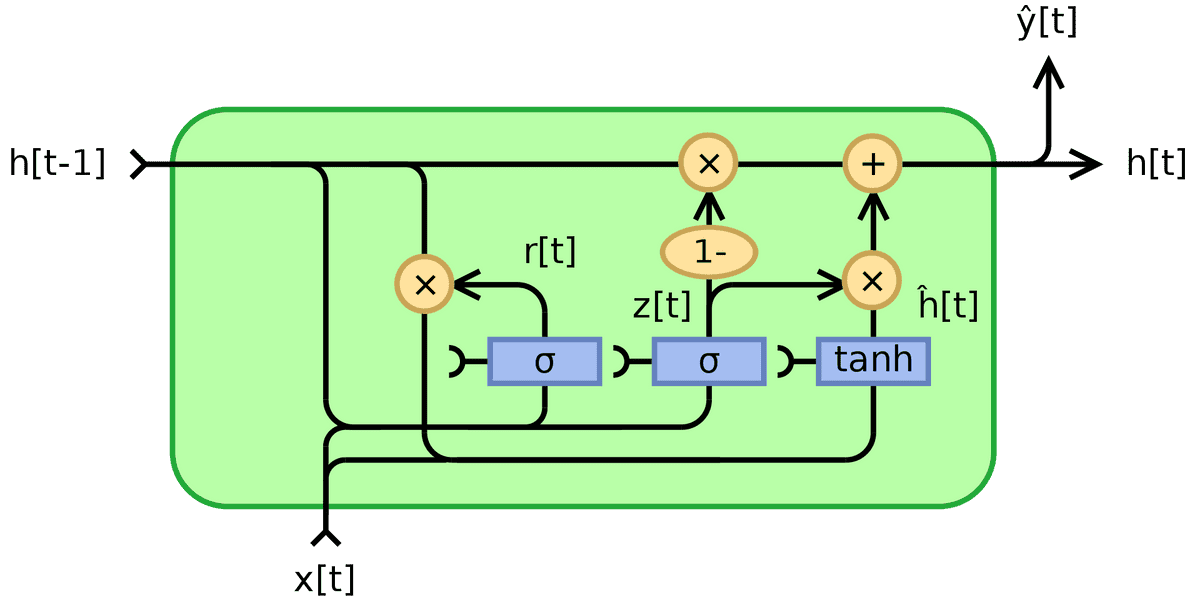
\includegraphics[width=0.5\textwidth]{Figuras/redes_neuronales/diagrama_celda_GRU.png}
    \caption{Esquema general de una célula GRU (Recuperado de Jeblad, CC BY-SA 4.0, \url{https://commons.wikimedia.org/w/index.php?curid=66234713}} 
    \label{fig:diagrama_GRU}
\end{figure}

\subsubsection{Entrenamiento de una red GRU}

En un sentido similar al desarrollo de entrenamiento de las redes LSTM, los gradientes de cada uno de los componentes de la célula son:

\begin{center}
    $\dfrac{\partial E}{g_t} = \dfrac{\partial E}{\partial h_t}(1-z_t)$
    
    $\dfrac{\partial E}{r_t} = \dfrac{\partial E}{\partial h_t}(1-z_t) W_g  h_{t-1} [1-g_t^2]$

    $\dfrac{\partial E}{z_t} = \dfrac{\partial E}{\partial h_t}(h_{t-1} - g_t)$
\end{center}

De la misma manera, los parámetros de la red quedan\footnote{Estos gradientes fueron recuperados de \cite{forward_and_Backprop_GRU_Mihir}.}:

\begin{center}
    $d1 = \dfrac{\partial E}{\partial h_t} (1-z_t) (1-g_t^2)$
    
    $d2 = [ [ ( d1 ) \odot W_h^T] h_{t-1}] (r_t(1-r_t))$

    $d3 = [h_{t-1}\dfrac{\partial E}{\partial h_t} - g_t\dfrac{\partial E}{\partial h_t}](z_t(1-z_t))$

    $\dfrac{\partial E}{W_r} = h_{t-1}^T \odot (d2)$

    $\dfrac{\partial E}{U_r} = x_t^T \odot (d2)$

    $\dfrac{\partial E}{W_z} = h_{t-1}^T \odot (d3)$

    $\dfrac{\partial E}{U_Z} = x_t^T \odot (d3)$

    $\dfrac{\partial E}{W_h} = h_{t-1}^T \odot (d1)$

    $\dfrac{\partial E}{U_h} = x_t^T \odot (d1)$
\end{center}

%problema del gradiente desvaneciente:




 % Experimental Setup

% !TEX root = ../Tesis.tex
\chapter{Construcción del Modelo} 
\label{cap:construccion} 

Los modelos que a continuación se presentan son compuestos por la DWT y cada una de las redes que estudiamos en el capítulo anterior: la NARNN, con la arquitectura propuesta por Asmaa Y. Fathi, et. al. \cite{DWT-NARNN} por un lado, y la estructura planteada por Adusumilli, R. \cite{ML_SP} para la la red con células LSTM (Long Short-Term Memory neural network) (LSTMnn) y la red con células GRU (GRUnn), así como las redes que no cuentan con el pre-procesamiento de datos de la DWT. 

Para la implementación, se usará \textit{Python 3.11} \footnote{El repositorio con el código del proyecto se puede ver en \url{https://github.com/MiguelAngelLiera/Stock_Exchange_NN_PP}.} \footnote{Las especificaciones del software utilizado se pueden ver en \ref{ApC}.} pues su sintaxis simple y legible facilita la programación y comprensión del código, lo que agiliza el desarrollo de los modelos de redes neuronales. Además cuenta con una cantidad importante de módulos y marcos de trabajo específicamente diseñados para el desarrollo de aprendizaje profundo. Algunos de los más populares incluyen TensorFlow, PyTorch, Keras, y scikit-learn (que revisaremos más adelante). Cada uno de ellos los iremos mencionado a medida que se requieran. Otra ventaja de su versatilidad es que permite combinar el uso de bibliotecas específicas con otras funcionalidades propias del lenguaje, como manipulación de datos y visualización de resultados en un mismo entorno.

\newpage

\section{Descomposición de datos por DWT}

A partir de este punto, se usarán los datos de \textbf{ACTINVRB} para cada uno de los pasos en la construcción de este y el siguiente capítulo. En este sentido, es un buen conjunto para la evaluación de los modelos desde que vemos la caída del valor de las acciones desde finales de 2019 (A partir de las doscientas semanas), hecho que se acentúa durante el primer año de la pandemia causada por la COVID-19. En palabras de Pablo Duarte, Director de Análisis y Estrategia de ACTINVER: "...la pandemia agregó mayor incertidumbre a las expectativas de crecimiento nacionales, mermando el ánimo de los inversionistas ya cautelosos por la crisis sanitaria." \cite{oportunidades_Actinver} Esta característica nos permite evaluar cómo reaccionan las arquitecturas ante eventos anómalos.

\begin{figure}[h]
    \centering
    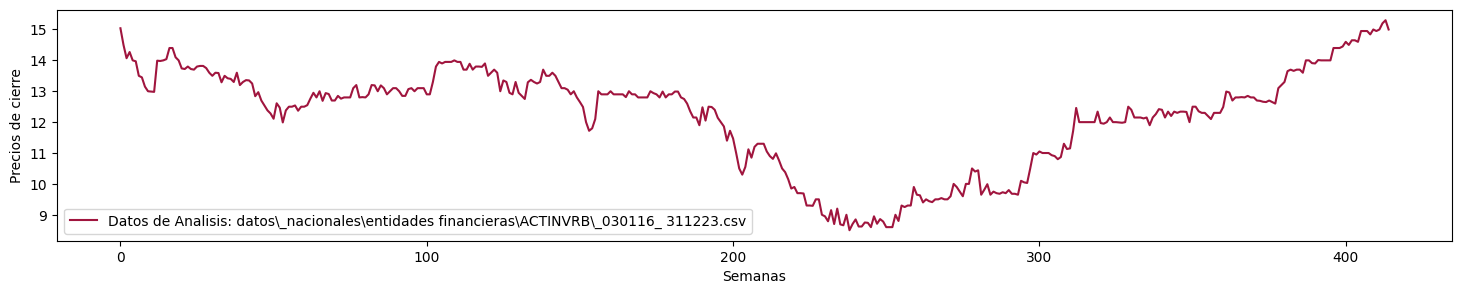
\includegraphics[width=1\textwidth]{Figuras/construccion_del_modelo/ACTINVR_030116_311223.png}
    \caption{Precios de cierre semanal de \textbf{ACTINVRB} del 1 de enero de 2016 al 31 de diciembre de 2023} 
    \label{fig:ACTINVRB}
\end{figure}

La biblioteca \textit{Pywavelets} \cite{pywavelets} cuenta con una implementación solida, eficiente y fácil de usar de algoritmos basados en ondículas tanto para análisis en tiempo continuo como en tiempo discreto. Proporciona una amplia gama de funciones para realizar transformaciones de ondícula y manipular coeficientes. Entre éstas podemos encontrar tanto para la descomposición de datos por DWT (función \texttt{dwt}) %\url{https://pywavelets.readthedocs.io/en/latest/ref/dwt-discrete-wavelet-transform.html#pywt.dwt}) 
 como para la reconstrucción de estos a partir de sus coeficientes (\texttt{idwt}, \texttt{upcoef}).

El primer paso de la descomposición es la elección de la ondícula madre. Se opta por una u otra dependiendo de las características de la serie de tiempo que se va a analizar. En general, debe ser en función del comportamiento de la serie original para que ésta pueda ser reconstruida o analizada. Para series que impliquen cambios no suaves y repentinos es recomendable usar \textit{bior3.5} \cite{DWT-NARNN}. Se trata de una ondícula madre que pertenece a la familia de ondículas biortogonales. La notación \textit{bior3.5} indica que tiene un filtro de paso bajo de longitud tres y un filtro de paso alto de longitud cinco en la descomposición, es decir, un filtro de tres coeficientes para la suavización (filtro de paso bajo) y un filtro de cinco coeficientes para la detección de detalles (filtro de paso alto). Así, nos da una buena representación de señales con cambios abruptos, lo que la hace útil en aplicaciones donde se requiere una alta capacidad de representación.

\begin{figure}[h]
    \centering
    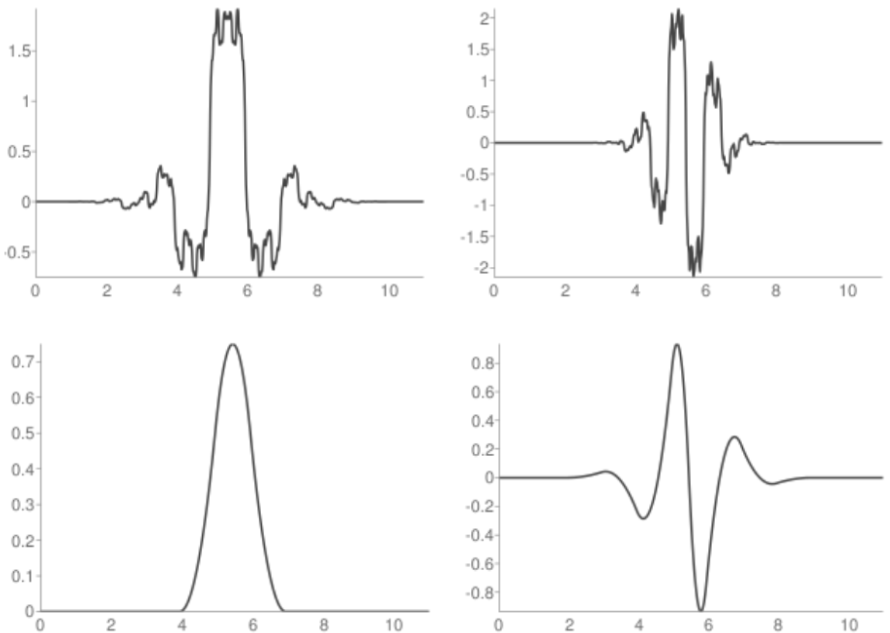
\includegraphics[width=0.7\textwidth]{Figuras/construccion_del_modelo/bior3.5.png}
    \caption{Funciones de descomposición (superior) y reconstrucción (inferior) de escala $\phi$ y de ondícula $\psi$. } 
    \label{fig:bior3_5}
\end{figure}

Para aplicar la DWT sobre los datos, es necesario realizar una extrapolación de los datos para que la descomposición en los extremos de la señal sea lo más precisa y limpia posible. Para nuestros fines, se escoge el modo \textit{symmetric} ya que refleja de mejor manera la descomposición en componentes de baja frecuencia.

\begin{figure}[h]
    \centering
    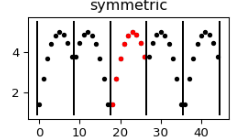
\includegraphics[width=0.5\textwidth]{Figuras/construccion_del_modelo/symmetric_pad_DWT.png}
    \caption{Extrapolación con modo \textit{Symmetric}.} 
    \label{fig:symmetric_pad}
\end{figure}

\newpage

\begin{figure}[h]
    \centering
    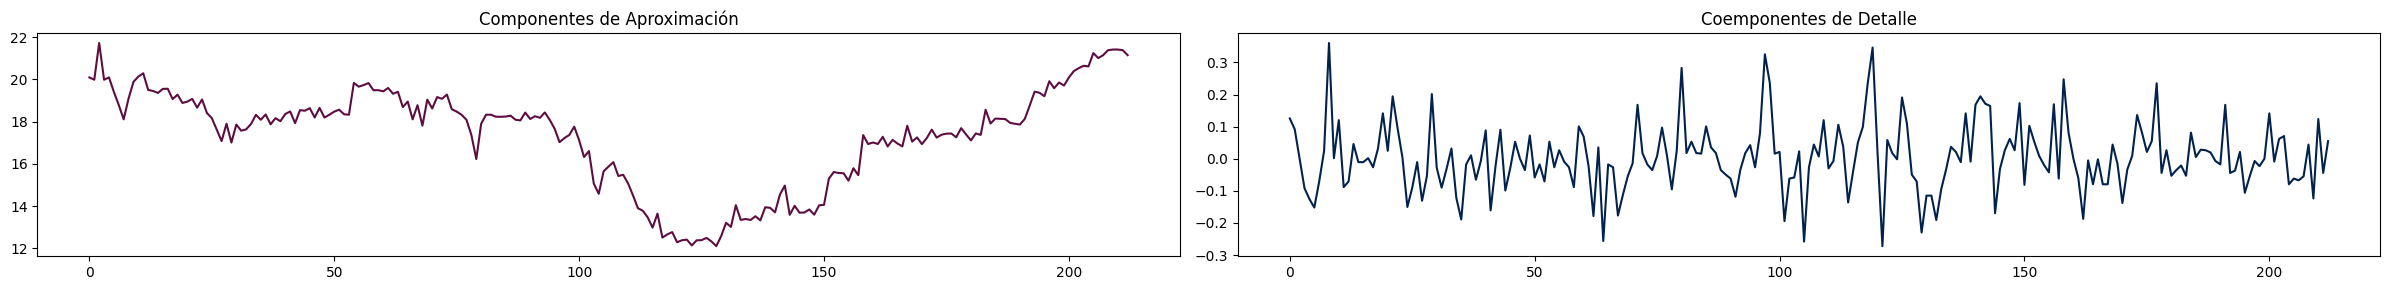
\includegraphics[width=1\textwidth]{Figuras/construccion_del_modelo/ACTINVR_DWT_lvl1.png}
    \caption{Componentes de Detalle y Aproximación de los datos de \textbf{ACTINVRB}.} 
    \label{fig:ACTINVRB_DWT_nivel1}
\end{figure}

Antes de continuar necesitamos dividir el conjunto de datos en entrenamiento (70$\%$) y prueba (30$\%$), para la fase del entrenamiento. Más adelante, durante el capítulo cinco \ref{cap:entrenamiento} se explica a detalle esta división.

\begin{figure}[h]
    \centering
    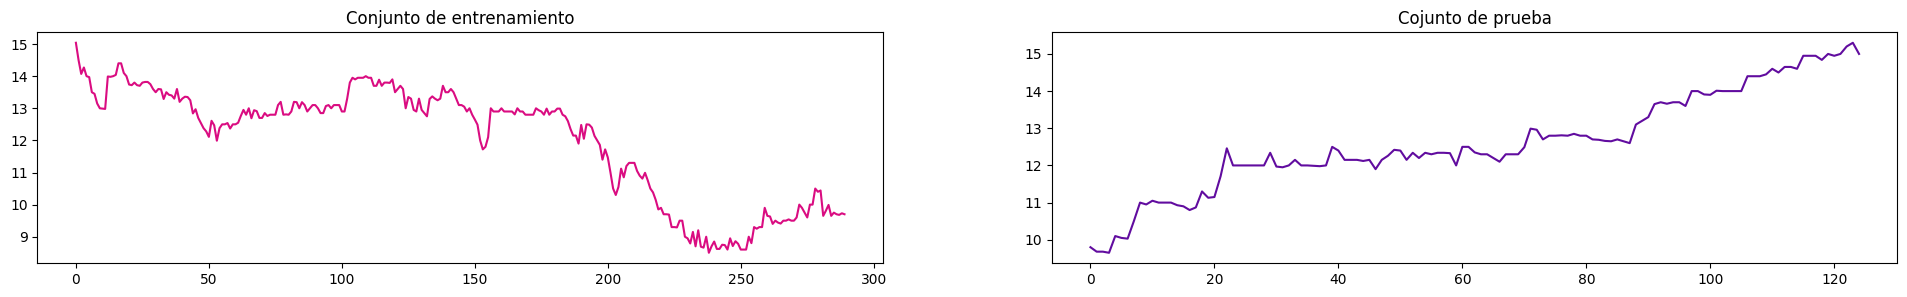
\includegraphics[width=1\textwidth]{Figuras/construccion_del_modelo/ACTINVR_entrenamiento_prueba.png}
    \caption{Conjunto de entrenamiento y prueba de los datos de \textbf{ACTINVRB}.} 
    \label{fig:ACTINVRB_entrenamiento_prueba}
\end{figure}

Para la eliminación del ruido de la señal, usaremos una descomposición en cinco niveles empleando el algoritmo piramidal que se mencionó en capítulos anteriores, atendiendo al hecho de suavizar la serie sin que pierda sus propiedades \footnote{La implementación de la descomposición multinivel de la señal por la DWT se puede encontrar en \ref{ApB}.}.

\begin{figure}[h]
    \centering
    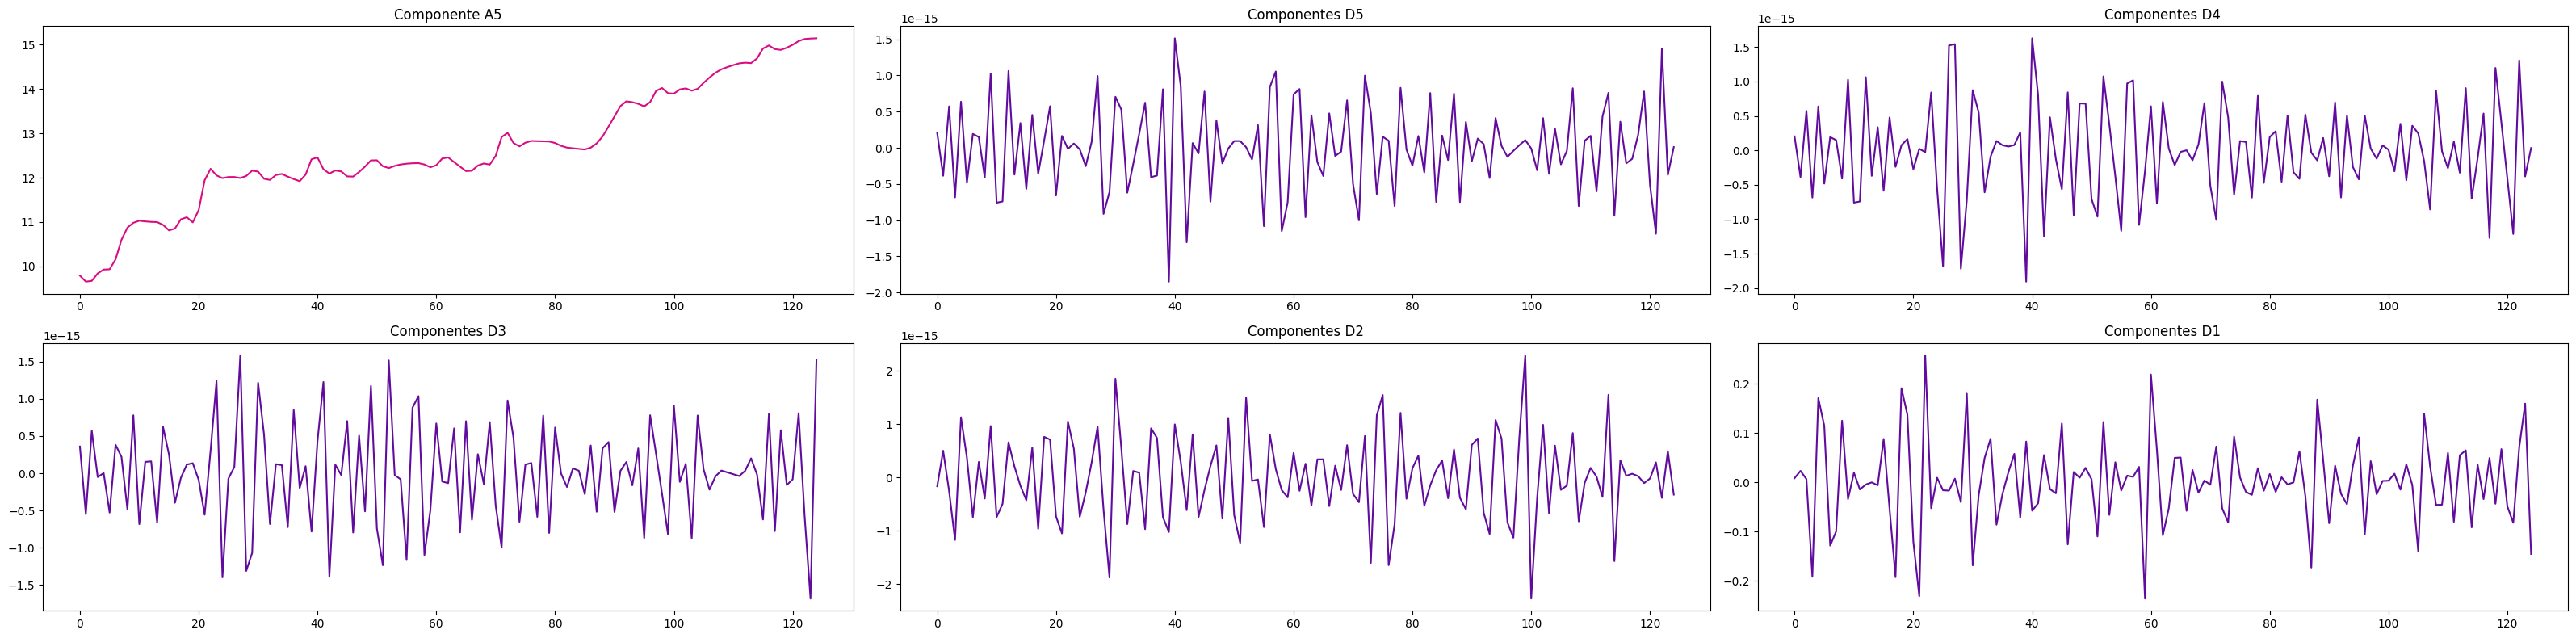
\includegraphics[width=1\textwidth]{Figuras/construccion_del_modelo/ACTINVR_prueba_DWT_lvl5.png}
    \caption{Componentes de detalle y aproximación en cinco niveles del conjunto de datos de prueba de \textbf{ACTINVRB}.} 
    \label{fig:ACTINVRB_prueba_DWT_nivel1_5}
\end{figure}

Para cada uno de estos componentes se creará una red NARNN, LSTMnn y GRUnn con el objetivo de pronosticar su comportamiento.

\newpage

\section{Modelo NARNN}

La arquitectura del modelo DWT-NARNN

\begin{figure}[H]
    \centering
    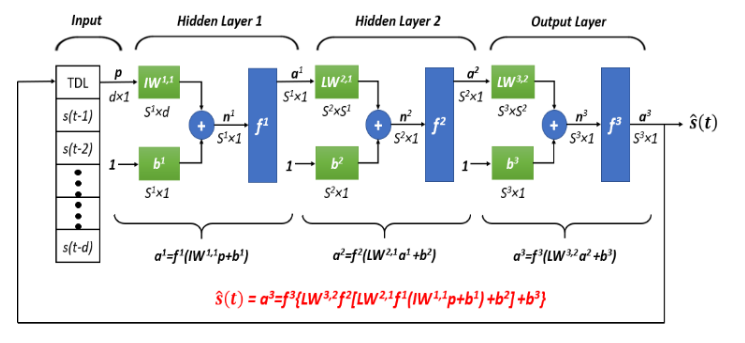
\includegraphics[width=0.8\textwidth]{Figuras/construccion_del_modelo/DWT-NARRN.png}
    \caption{Arquitectura NARNN (Recuperado de \cite{DWT-NARNN}).} 
    \label{fig:arquitectura_NARNN}
\end{figure}

En la figura \ref{fig:arquitectura_NARNN} podremos encontrar la arquitectura de la NARNN. Se trata de RNN con una Linea de Tiempo Retrasado (LTR) que representa los datos cierre de las ocho semanas anteriores a la predicción. También encontramos dos capas ocultas cada una con diez neuronas típicas y una última capa de salida con una sola neurona. Los sesgos de las neuronas en cada capa están representados por el vector $b$ y los respectivos pesos por los vectores $IW$ \textit{pesos de entrada} o \textit{input weights} y $LW$ \textit{pesos de capa} o \textit{layer weights} según la notación de Asmaa Y. Fathi, et. al. La función de activación en cada capa es la \textit{logaritmica-sigmoide}, \textit{tangente hiperbólica sigmoide}\footnote{Ambas funciones son versiones alternativas de la función sigmoide. Toman la composición de la primera en la segunda funcion, es decir:
\[
TanhSigmoide(x) = tanh\left[\dfrac{1}{e^{-x} + 1}\right]
\]\[
LogSigmoide(x) =log\left[\dfrac{1}{e^{-x} + 1}\right]
\]

Son efectivas para normalizar los datos y suavizar las pre-activaciones que reciben.
} y una función lineal respectivamente.

Para su implementación se utilizó la biblioteca \textit{pytorch} \footnote{Esta desición parte de la necesidad de crear un entrenamiento único (ya que se implementa el algoritmo LM para la parte entrenamiento) en comparación de las redes recurrentes.} \ref{ApB}.


\section{Modelo LSTMnn}

La red LSTMnn se toma la arquitectura:

\begin{figure}[H]
    \centering
    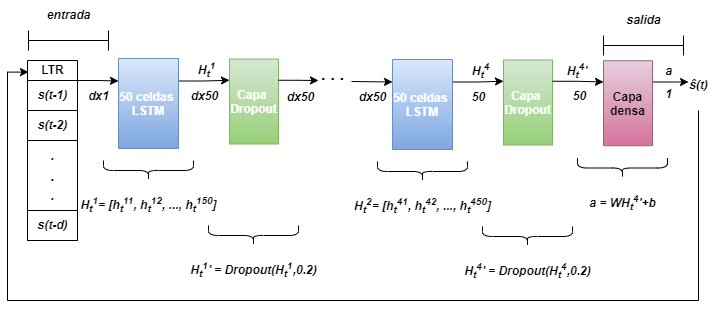
\includegraphics[width=0.8\textwidth]{Figuras/construccion_del_modelo/LSTMnn_arquitectura.png}
    \caption{Arquitectura LSTMnn.} 
    \label{fig:arquitectura_LSTMnn}
\end{figure}

La LSTMnn, al igual que la NARNN, presenta una LTR. Los ocho datos de entrada serán procesados por cuatro capas (células LSTM) con cincuenta unidades de salida cada una, y entre ellas cuatro capas de exclusión aleatorio o \textit{dropout} al veinte por ciento, de manera que esta cantidad de respuestas de la capa inmediata anterior se trunquen a cero para evitar el sobre-ajuste. Finalmente encontramos una capa densamente conectada con una sola neurona para la salida.

La implementación fue resuelta a partir de la biblioteca \textit{keras} \footnote{Gracias a que este marco de trabajo nos brinda una implementación solida de las LSTMnn y las GRUnn se decidió su uso.}. Se implementa la LSTMnn en \ref{ApB}.

\section{Modelo GRUnn}

Es una arquitectura par a la LSTMnn con la diferencia de que las capas con células LSTM son remplazadas por capas GRU, esto para mostrar una comparación equivalente y transparente entre el par de redes recurrentes. La red GRUnn se toma la arquitectura:

\begin{figure}[H]
    \centering
    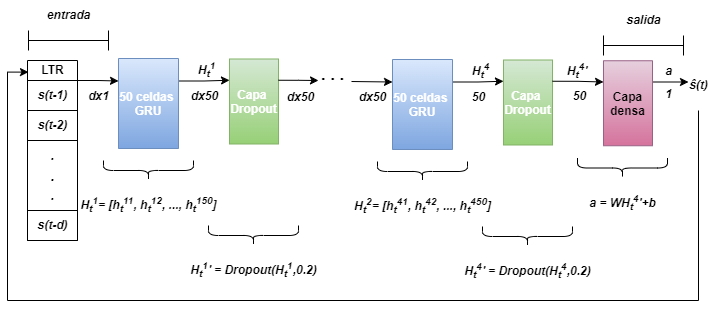
\includegraphics[width=0.8\textwidth]{Figuras/construccion_del_modelo/GRUnn_arquitectura.png}
    \caption{Arquitectura GRUnn.} 
    \label{fig:arquitectura_GRUnn} 
\end{figure}

La implementación fue resuelta a partir de la biblioteca \textit{keras}. Se implementa la GRUnn en \ref{ApB}.




 % Experiment 1

% !TEX root = ../Tesis.tex
\chapter{Proceso de Entrenamiento} 
\label{cap:entrenamiento} 

El método de entrenamiento es a la par de importante que la elección de la arquitectura y paradigma de la red. El algoritmo de optimización, sumado a los parámetros que se usarán: tasa de aprendizaje, épocas, tamaño de lote son determinantes en el resultado del experimento. En el caso de las NARNNs, es la propagación hacia atrás partiendo del algoritmo Levenverg-Marquardt \footnote{Cuya implementación se ve reflejada en \ref{ApB}} el proceso empleado. Mientras que ADAM es utilizado en el aprendizaje de las RNNs. Aunado a lo anterior, nos valdremos de metodologías sobre el proceso: el entrenamiento por reforzamiento del profesor y el entrenamiento auto-predictivo, además de un análisis exhaustivo para hallar los parámetros ideales.

Para estos dos enfoques se emplearán dos tipos de muestreos. Primero, procederemos partiendo el conjunto de datos en dos: una para el entrenamiento que comprende el setenta por ciento de este, tomando las muestras de forma aleatoria y lo mismo para el restante conjunto de prueba. Nos referiremos a esta propuesta como \textit{muestreo aleatorio}. Luego se evaluará el desempeño de los modelos sobre estos datos en diferentes combinaciones de parámetros (tasa de aprendizaje y épocas). Posterior a ello, dividiremos nuevamente los conjuntos en la misma proporción, pero con la diferencia que separaremos el conjunto de manera temporal: el último treinta por ciento de la serie de tiempo, que serán nuestras últimas semanas de análisis formarán parte del conjunto de prueba, sea \textit{muestro temporal}, y de igual manera se examinarán los resultados \footnote{A lo largo de este capitulo se muestran los resultados de las predicciones sobre los conjuntos de entrenamiento co0n estos dos muestreos.}.

Para comparar el rendimiento de los modelos tomaremos como métricas de comparación durante el entrenamiento al error cuadrático medio (\textit{Mean Square Error}) (MSE) pues es tanto para las NARNNs y como para las RNNs su función de error, además que es una medida simple para medir el error en la predicción a priori. Esta medida se verá reflejada en las gráficas del presente capítulo.

Por otro lado para tratar a mayor profundidad el análisis en relación a las pruebas nos valdremos de otras tres métricas que se verán reflejadas en el siguiente capítulo: la raíz del error cuadrático medio (\textit{Rooted Mean Squared Error}) (RMSE) como una versión alterna al MSE. El porcentaje promedio de error absoluto (\textit{Mean Absolute Percentage Error}) (MAPE) que describe la magnitud promedio del error absoluto del modelo. La Simetría Direccional (\textit{Directional Symmetry}) (DS) es una medida que evalúa la dirección del pronóstico respecto a la dirección real de cambio en la serie de tiempo:

\begin{center}
    RMSE = $\sqrt{\frac{1}{n} \sum_{i=1}^{n} (y_i - \hat{y}_i)^2}$

    MSE = $\frac{1}{n} \sum_{i=1}^{n} (y_i - \hat{y}_i)^2$

    MAPE = $\frac{1}{n} \sum_{i=1}^{n} \left| \frac{y_i - \hat{y}_i}{y_i} \right| \times 100$
    
    DS = $\frac{100}{n} \sum_{i=1}^{n} d_i$
\end{center}

Donde:
\begin{itemize}
    \item $n$: Número total de observaciones.
    \item $y_i$: Valor real o verdadero en la observación $i$.
    \item $\hat{y_i}$: Valor predicho por el modelo para la observación $i$.
    \item \[
    d_i = 
    \begin{cases}
    1, & \text{si } (y_{i}-y_{t-1})(\hat{y_{i}}-\hat{y_{t-1}}) \geq 0 \\
    0, & \text{de otra manera}
    \end{cases}
    \]
\end{itemize}

Como se mencionó, para cada método de entrenamiento se encontraron los parámetros adecuados a partir de una búsqueda exhaustiva de la mejor combinación de estos para lograr una predicción aceptable y evitando el sobre-ajuste. Dicho procedimiento se ve reflejado en las tablas de referencia que se ven a continuación (tasa de aprendizaje contra número de épocas) en las cuales se vera reflejado el MSE total de la predicción y en el caso de los modelos que cuentan una descomposición con la DWT se presenta MSE de los componentes / MSE de la reconstrucción.

\newpage

\section{Entrenamiento por reforzamiento del profesor}

Cada característica del conjunto de datos, es decir, la entrada de la red en cualquier lote de alguna época del entrenamiento, forma parte de los datos originales: el precio de cierre semanal durante ocho semanas ($[t_{n-1}, t_{n-2}, ...,t_{n-8}]$). A partir de estas se dará como salida el valor de la novena semana ($t_n$). Durante el ajuste de parámetros, la técnica de reforzamiento del profesor se emplea entrenando al modelo utilizando los valores reales del conjunto y no las salidas del modelo. De esta manera, se emplea un corrimiento temporal del valor de una semana durante la evaluación de la siguiente característica ( tomando $[t_{(n+1)-1}, t_{(n+1)-2}, ...,t_{(n+1)-8}]$, los inmediatos anteriores originales del conjunto sin tomar en cuenta ninguna predicción), para predecir la consecuente ($t_{n+1}$). 

\begin{figure}[H]
    \centering
    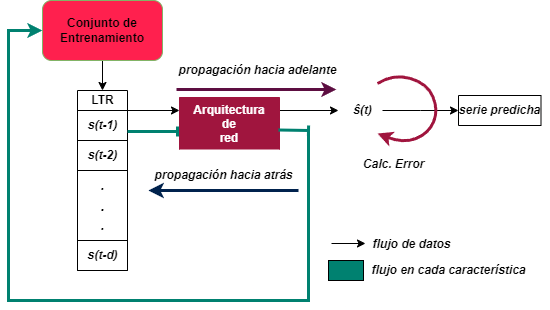
\includegraphics[width=0.8\textwidth]{Figuras/proceso_de_entrenamiento/Reforzamiento_del_profesor.png}
    \caption{Diagrama del reforzamiento del profesor.} 
    \label{fig:reforzamiento_profesor}
\end{figure}

\newpage
%%%%%%%%%%%%%%%%%%%%%%%%%%%%%%%%%%%%%%%%%
\subsection{NARNN}

Cuando todas las características del lote cuentan con su correspondiente predicción es cuando LM ejecuta un paso, modificando los pesos y sesgos de la red a partir del gradiente y matriz hessiana de la función de error.

Para encontrar el conjunto adecuado de hiper-parámetros para la fase de optimización, se analizó la combinación de la tasa de aprendizaje contra el número de épocas, manteniendo un tamaño de lote de uno. Comenzamos arbitrariamente en cualquier punto de la tabla, y se direcciona la búsqueda hacia donde el error en cada época parezca disminuir lo suficiente.

\begin{figure}[H]
    \centering
    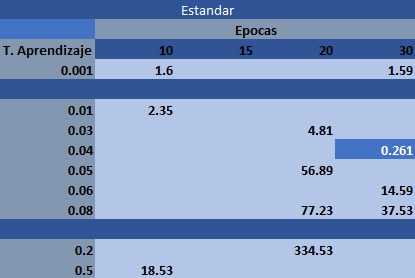
\includegraphics[width=0.7\textwidth]{Figuras/proceso_de_entrenamiento/lr_epocas_NARNN_estandar.png}
    \caption{Tabla comparativa entre combinaciones de parámetros de la NARNN: tasa de aprendizaje contra número épocas} 
    \label{fig:lr_epocas_NARNN}
\end{figure}

Como vemos, la mejor intersección se da en [0.04,30]. Para ilustrar que tan bien logrado es el entrenamiento a priori, se obtuvieron las siguientes predicciones sobre el mismo conjunto de entrenamiento en ambos tipos muestreos:

\begin{figure}[H]
    \begin{minipage}{0.5\textwidth}
        \centering
        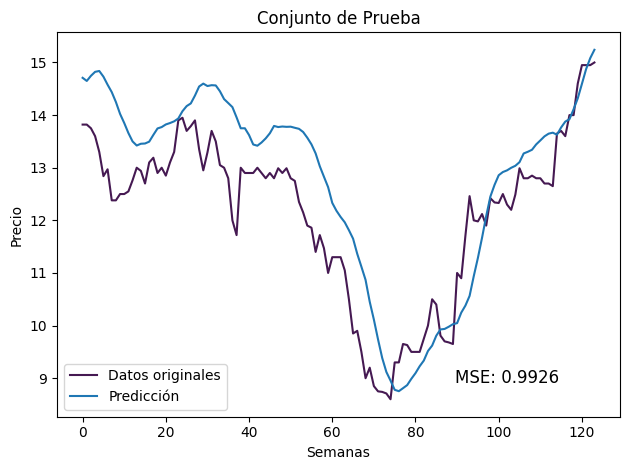
\includegraphics[width=\linewidth]{Figuras/proceso_de_entrenamiento/grafs_c_prueba/muestreo_aleatorio/NARNN/estandar/NARNN.png}
    \end{minipage}
    \begin{minipage}{0.5\textwidth}
        \centering
        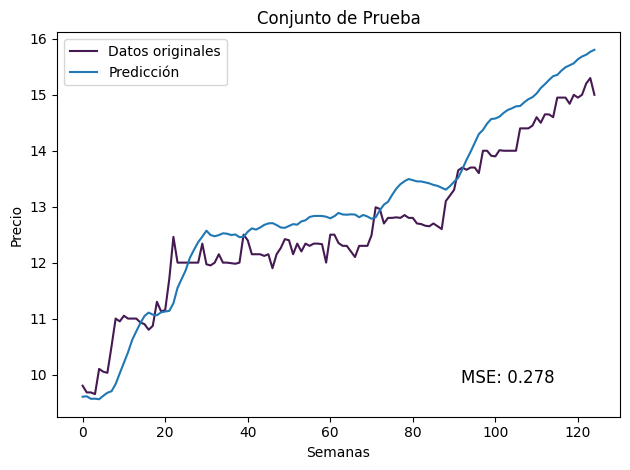
\includegraphics[width=\linewidth]{Figuras/proceso_de_entrenamiento/grafs_c_prueba/NARNN/estandar/NARNN.png}
        
    \end{minipage}
    \caption{Desempeño de la NARNN en conjunto de prueba: Muestro aleatorio y temporal} 
    \label{fig:c_prueba_NARNN}
\end{figure}

Cabe mencionar que encontrar los parámetros adecuados depende directamente de como estén inicializados estos. En general, para tanto la NARNN y la DWT-NARNN y para la longitud de datos de estudio representa un reto importante a la hora de encontrarlos \footnote{Como se ve reflejado en la tabla, el número de intentos en comparación a los de las RNNs es mayor}. 

En general las predicciones de NARNN son bastante aceptables, captando la dirección y comportamiento de la serie. Sin embargo, falla en captar los elementos 'sorpresivos' a los que este tipo de datos se atienen, como es el caso de los numerosos picos y hendiduras del muestreo temporal de las semanas veinte a ochenta.

\newpage

\subsection{DWT-NARNN}
Se procedió de manera similar que la NARNN, con la diferencia que se encontraron diferentes combinaciones de parámetros para las redes dedicadas a los componentes de detalle y de aproximación.

\begin{figure}[H]
    \centering
    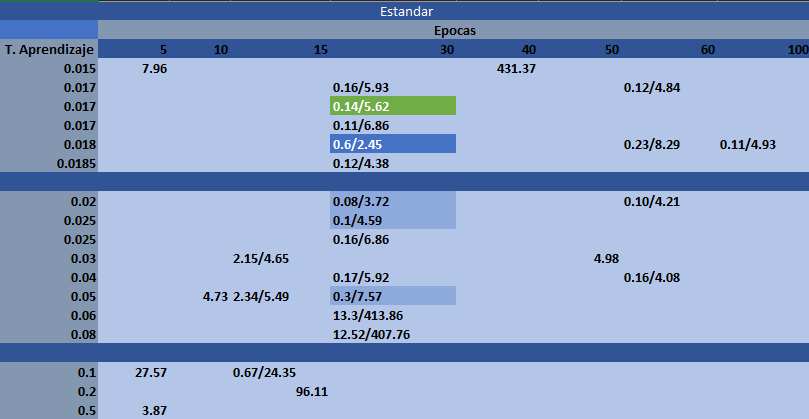
\includegraphics[width=0.7\textwidth]{Figuras/proceso_de_entrenamiento/lr_epocas_DWT_NARNN_estandar.png}
    \caption{Tabla comparativa entre combinaciones de parámetros de la DWT-NARNN: tasa de aprendizaje contra número épocas. (Los datos resaltados en verde representan la mejor combinaciones para las componentes de alta frecuencia y azul para los de baja).} 
    \label{fig:lr_epocas_DWTNARNN}
\end{figure}

\begin{figure}[H]
    \centering
    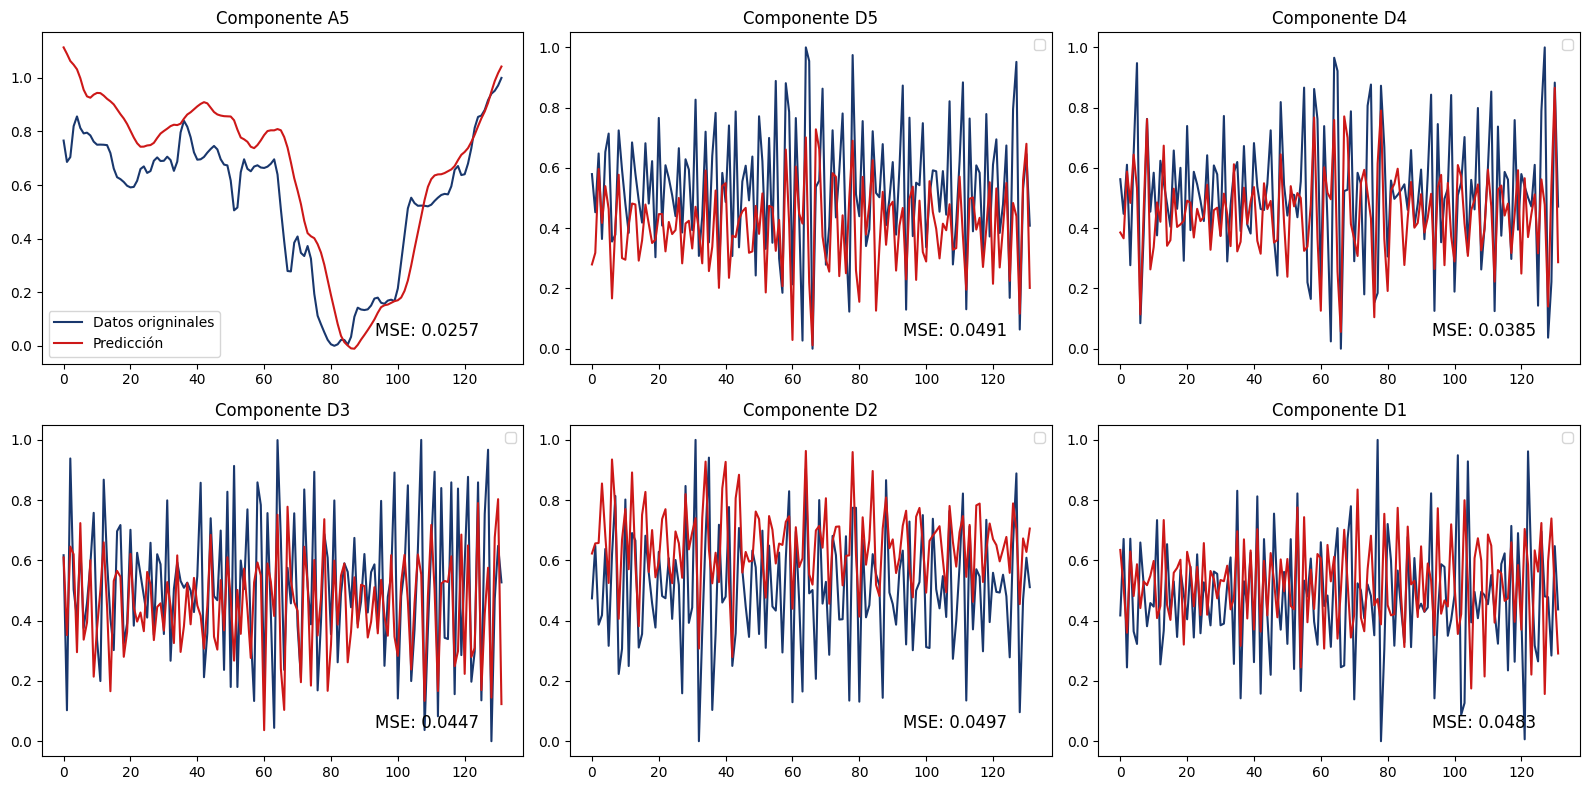
\includegraphics[width=0.9\textwidth]{Figuras/proceso_de_entrenamiento/grafs_c_prueba/muestreo_aleatorio/DWT_NARNN/estandar/DWT_NARNN.png}
    \caption{Predicciones de la DWT-LSTMnn de los componentes del conjunto de pruebas de muestro aleatorio.} 
    \label{fig:c_prueba_componentes_DWT_NARNN_aleatorio}
\end{figure}

\begin{figure}[H]
    \centering
    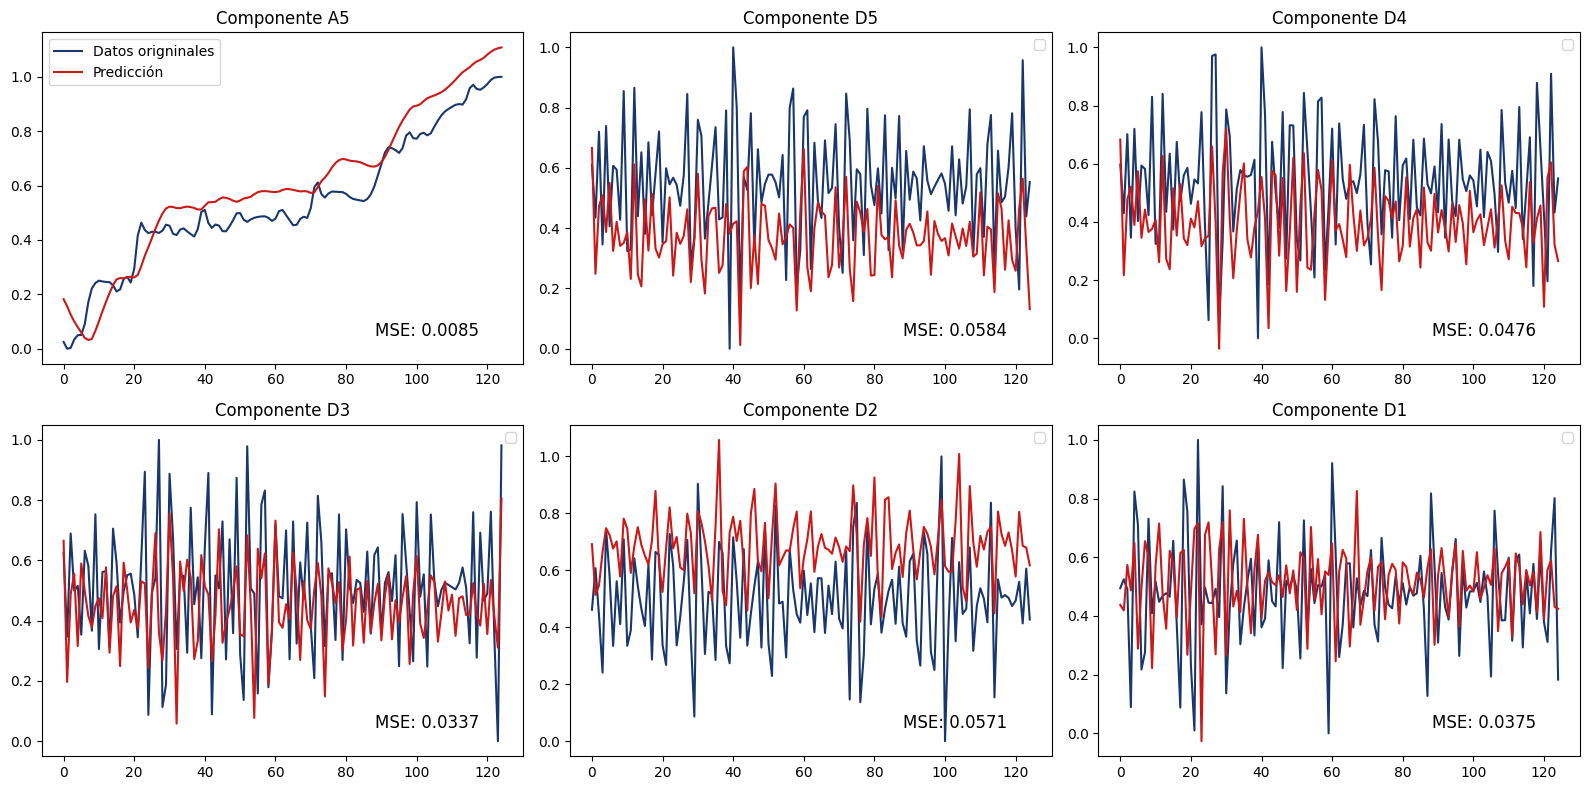
\includegraphics[width=0.9\textwidth]{Figuras/proceso_de_entrenamiento/grafs_c_prueba/DWT_NARNN/estandar/DWT_NARNN.png}
    \caption{Predicciones de la DWT-LSTMnn de los componentes del conjunto de pruebas de muestro temporal.} 
    \label{fig:c_prueba_componentes_DWT_NARNN}
\end{figure}

\begin{figure}[H]
    \begin{minipage}{0.5\textwidth}
        \centering
        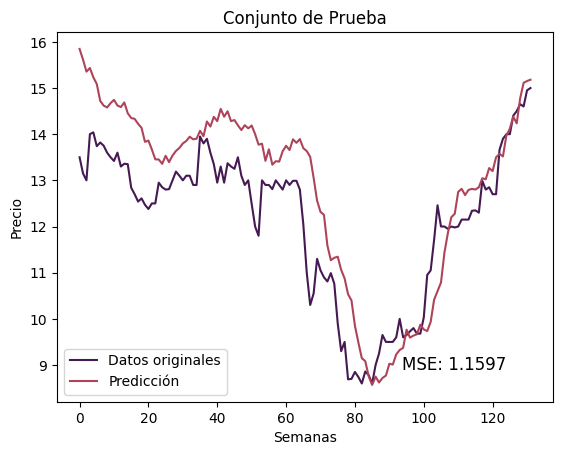
\includegraphics[width=\linewidth]{Figuras/proceso_de_entrenamiento/grafs_c_prueba/muestreo_aleatorio/DWT_NARNN/estandar/DWT_NARNN_rec.png}
    \end{minipage}
    \begin{minipage}{0.5\textwidth}
        \centering
        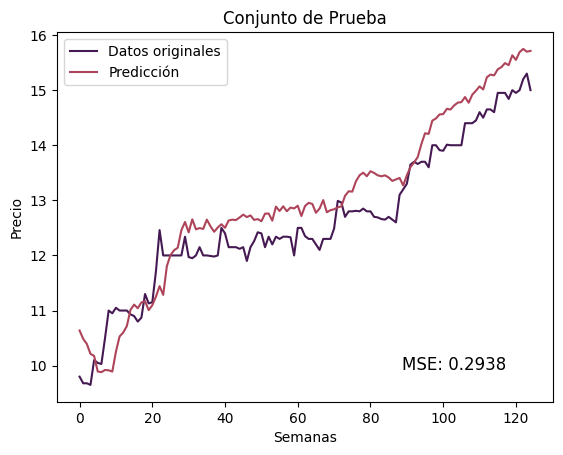
\includegraphics[width=\linewidth]{Figuras/proceso_de_entrenamiento/grafs_c_prueba/DWT_NARNN/estandar/DWT_NARNN_rec.png}
    \end{minipage}
    \caption{Desempeño de la DWT-NARNN en la reconstrucción del conjunto de prueba: Muestreo aleatorio y temporal.} 
    \label{fig:c_prueba_DWTNARNN}
\end{figure}

Se ve una notable mejoría en la captación de cambios subitos en las tendencias con respecto al modelo anterior, pero un aumento legero del error precisamente a estos cambios.

\newpage
%%%%%%%%%%%%%%%%%%%%%%%%%%%%%%%%%%%%%%%%%%%%%%%%%%%%%%%
\subsection{LSTMnn}

Encontrar los parámetros ideales en este caso empleó un menor esfuerzo. Partiendo de los datos que nos proporciona Adusumilli, Roshan, una tasa de aprendizaje de 0.0001, un tamaño de lote de 32 y 60 épocas, se obtuvieron muy buenos resultados en ambos muestreos:

\begin{figure}[H]
    \begin{minipage}{0.5\textwidth}
        \centering
        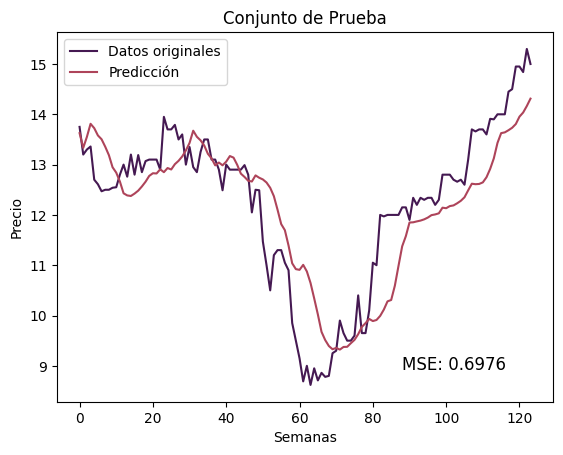
\includegraphics[width=\linewidth]{Figuras/proceso_de_entrenamiento/grafs_c_prueba/muestreo_aleatorio/LSTM/estandar/LSTM.png}
    \end{minipage}
    \begin{minipage}{0.5\textwidth}
        \centering
        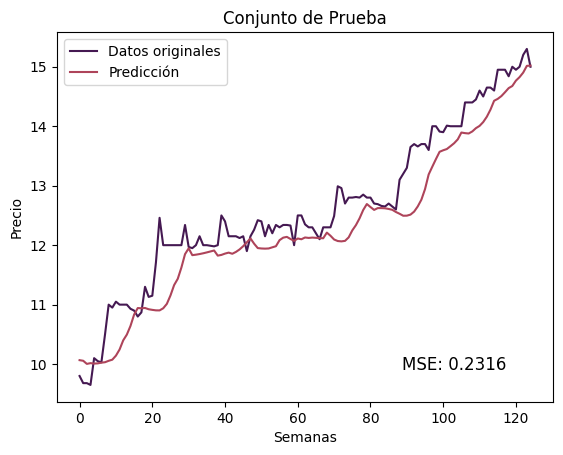
\includegraphics[width=\linewidth]{Figuras/proceso_de_entrenamiento/grafs_c_prueba/LSTM/estandar/LSTM.png}
    \end{minipage}
    \caption{Desempeño de la LSTMnn en conjunto de prueba: Muestreo aleatorio y temporal.} 
    \label{fig:c_prueba_LSTM}
\end{figure}

En comparación con los anteriores, mejora respecto a NARNN, pero sigue mostrando un poco de resistencia en ante cambios inesperados.

\newpage
%%%%%%%%%%%%%%%%%%%%%%%%%%%%%%%%%%%%%%%%%%%%%%%%%%%%%%%
\subsection{DWT-LSTMnn}

Se usaron los mismos parámetros que para la LSTMnn en la predicción de la componente \textit{A5} de baja frecuencia. Mientras que para las demás se procedió de manera similar a la NARNN y a la DWT-NARNN.

\begin{figure}[H]
    \centering
    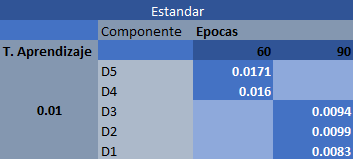
\includegraphics[width=0.5\textwidth]{Figuras/proceso_de_entrenamiento/lr_epocas_DWT_LSTM_estandar_componentes.png}
    \caption{Tabla comparativa entre parámetros para componentes de alta frecuencia de la DWT-LSTMnn: tasa de aprendizaje contra número épocas por cada componente.} 
    \label{fig:lr_epocas_DWT_LSTMnn_componentes}
\end{figure}

\begin{figure}[H]
    \centering
    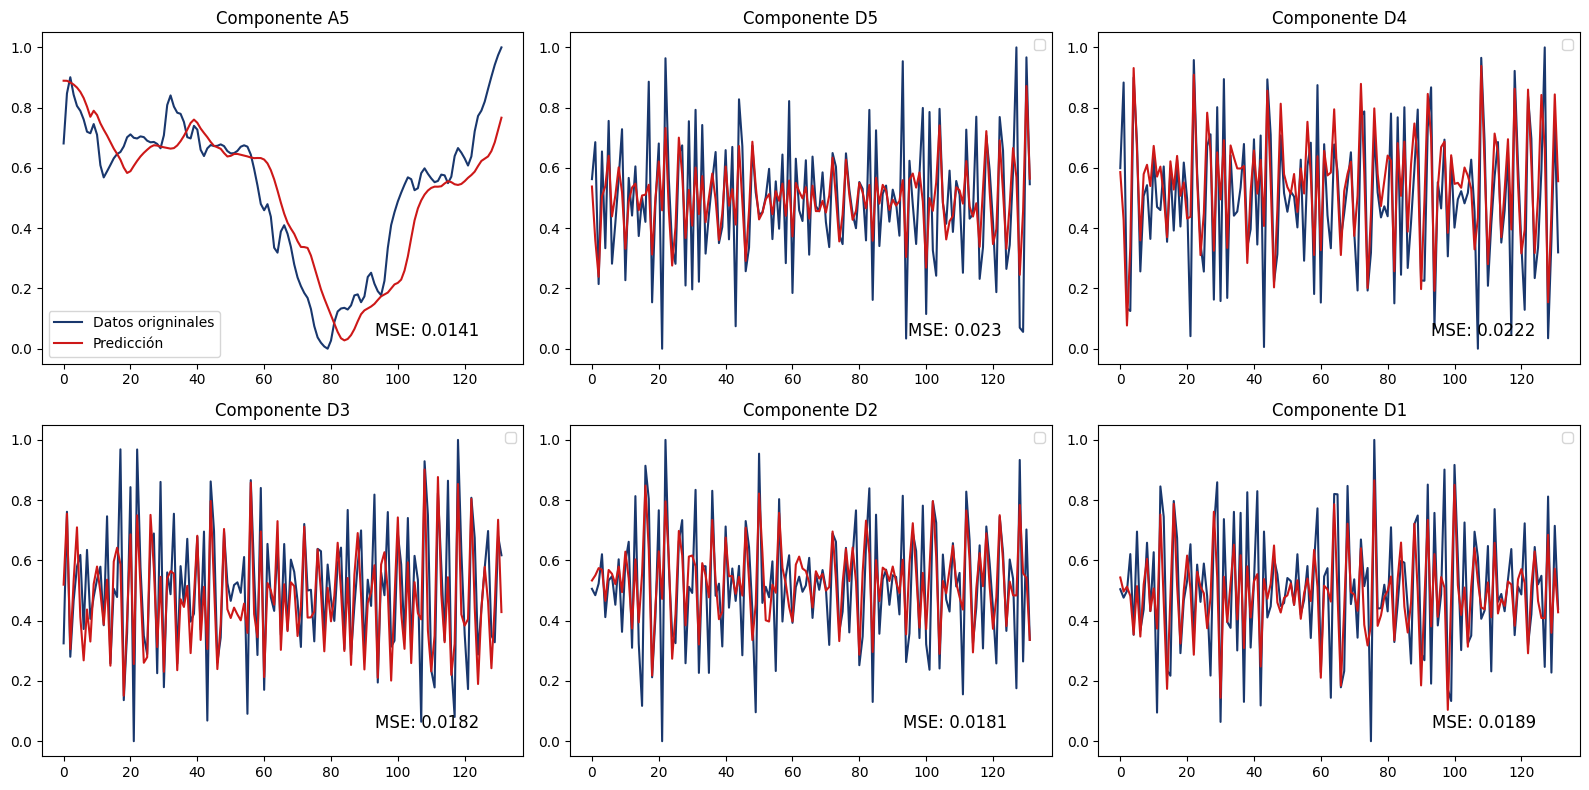
\includegraphics[width=0.9\textwidth]{Figuras/proceso_de_entrenamiento/grafs_c_prueba/muestreo_aleatorio/DWT_LSTM/estandar/DWT_LSTM.png}
    \caption{Predicciones de la DWT-LSTMnn de los componentes del conjunto de pruebas de muestro aleatorio.} 
    \label{fig:c_prueba_componentes_DWT_LSTM_aleatorio}
\end{figure}

\begin{figure}[H]
    \centering
    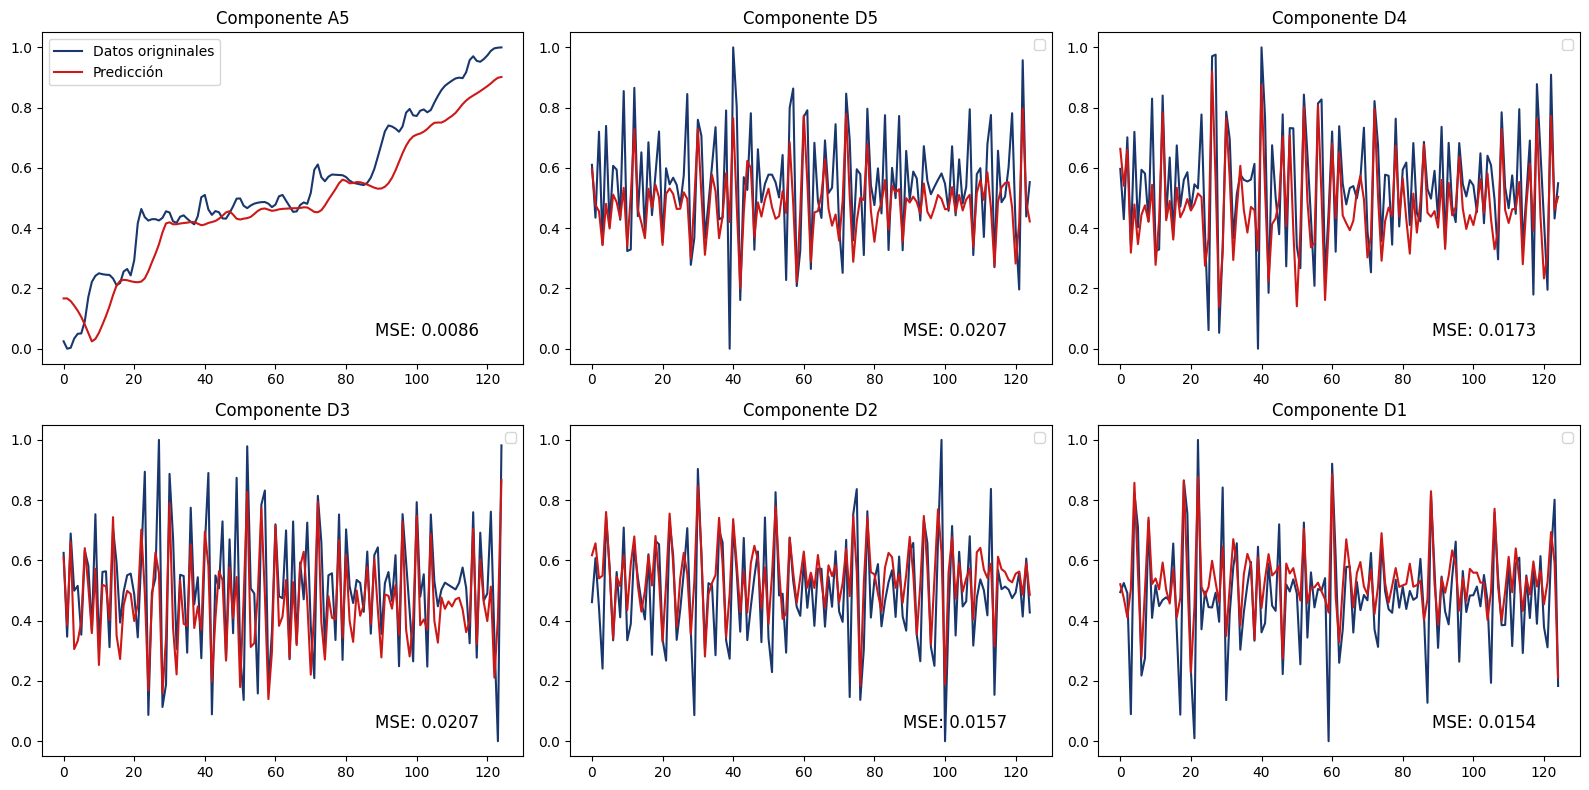
\includegraphics[width=0.9\textwidth]{Figuras/proceso_de_entrenamiento/grafs_c_prueba/DWT_LSTM/estandar/DWT_LSTM.png}
    \caption{Predicciones de la DWT-LSTMnn de los componentes del conjunto de pruebas de muestro temporal.} 
    \label{fig:c_prueba_componentes_DWT_LSTM}
\end{figure}

\begin{figure}[H]
    \begin{minipage}{0.5\textwidth}
        \centering
        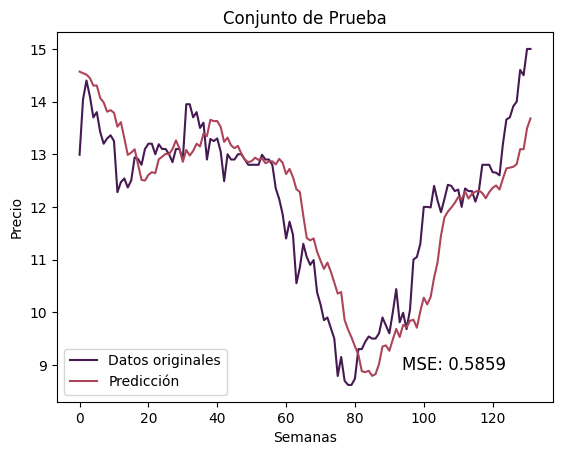
\includegraphics[width=\linewidth]{Figuras/proceso_de_entrenamiento/grafs_c_prueba/muestreo_aleatorio/DWT_LSTM/estandar/DWT_LSTM_rec.png}
    \end{minipage}
    \begin{minipage}{0.5\textwidth}
        \centering
        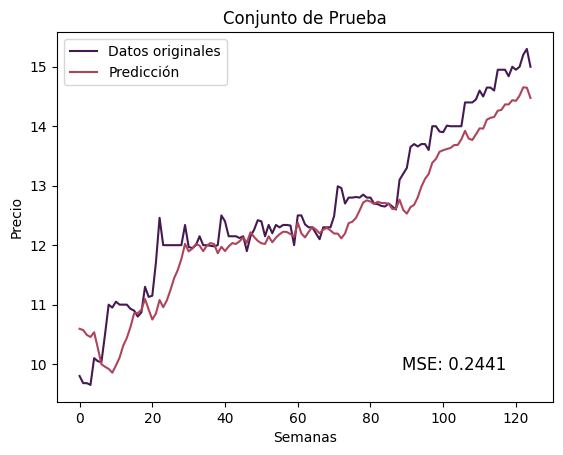
\includegraphics[width=\linewidth]{Figuras/proceso_de_entrenamiento/grafs_c_prueba/DWT_LSTM/estandar/DWT_LSTM_rec.png}
    \end{minipage}
    \caption{Desempeño de la DWT-LSTMnn en la reconstrucción del conjunto de prueba: Muestro aleatorio y temporal.} 
    \label{fig:c_prueba_DWTLSTM}
\end{figure}

Es clara la diferencia con DWT-NARNN, pues el error disminuye, y sigue manteniendo la capacidad de captar el 'ruido' de los datos. En ambos muestreos existen ventanas temporales donde la predicción se acerca bastante a los valores reales. Tal es el caso de las semanas treinta a sesenta del segundo ejemplo, posiblemente debido a el comportamiento en esos puntos.

\newpage
%%%%%%%%%%%%%%%%%%%%%%%%%%%%%%%%%%%%%%%%%%%%%%%%%%%%%%%
\subsection{GRUnn}

Al poseer una arquitectura paralela a las LSTMnn y la DWT-GRUnn a la DWT-LSTMnn, se hicieron uso de los mismos datos de entrenamiento. Obteniendo así:

\begin{figure}[H]
    \begin{minipage}{0.5\textwidth}
        \centering
        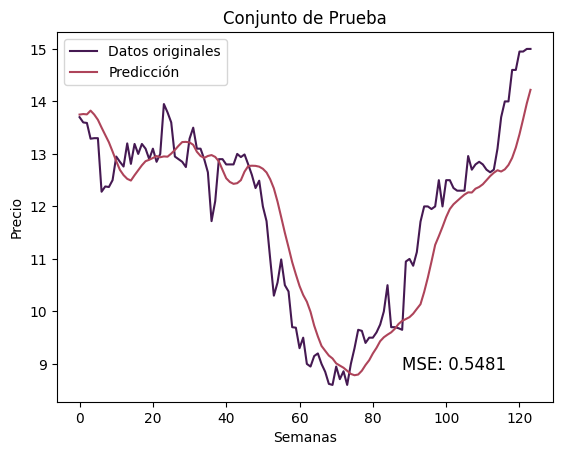
\includegraphics[width=\linewidth]{Figuras/proceso_de_entrenamiento/grafs_c_prueba/muestreo_aleatorio/GRU/estandar/GRU.png}
    \end{minipage}
    \begin{minipage}{0.5\textwidth}
        \centering
        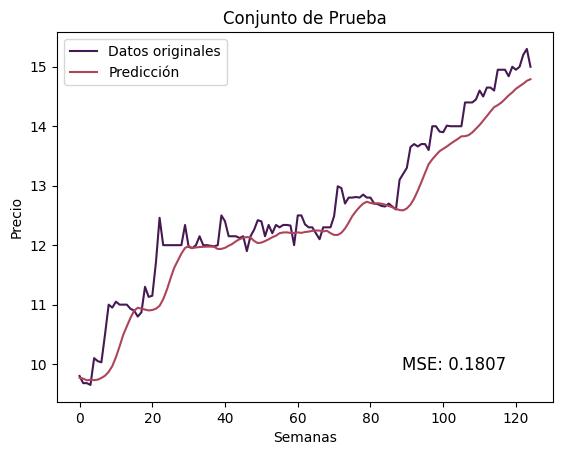
\includegraphics[width=\linewidth]{Figuras/proceso_de_entrenamiento/grafs_c_prueba/GRU/estandar/GRU.png}
    \end{minipage}
    \caption{Desempeño de la GRUnn en conjunto de prueba: Muestro aleatorio y temporal} 
    \label{fig:c_prueba_GRU}
\end{figure}

\newpage
%%%%%%%%%%%%%%%%%%%%%%%%%%%%%%%%%%%%%%%%%%%%%%%%%%%%%%%
\subsection{DWT-GRUnn}

\begin{figure}[H]
    \centering
    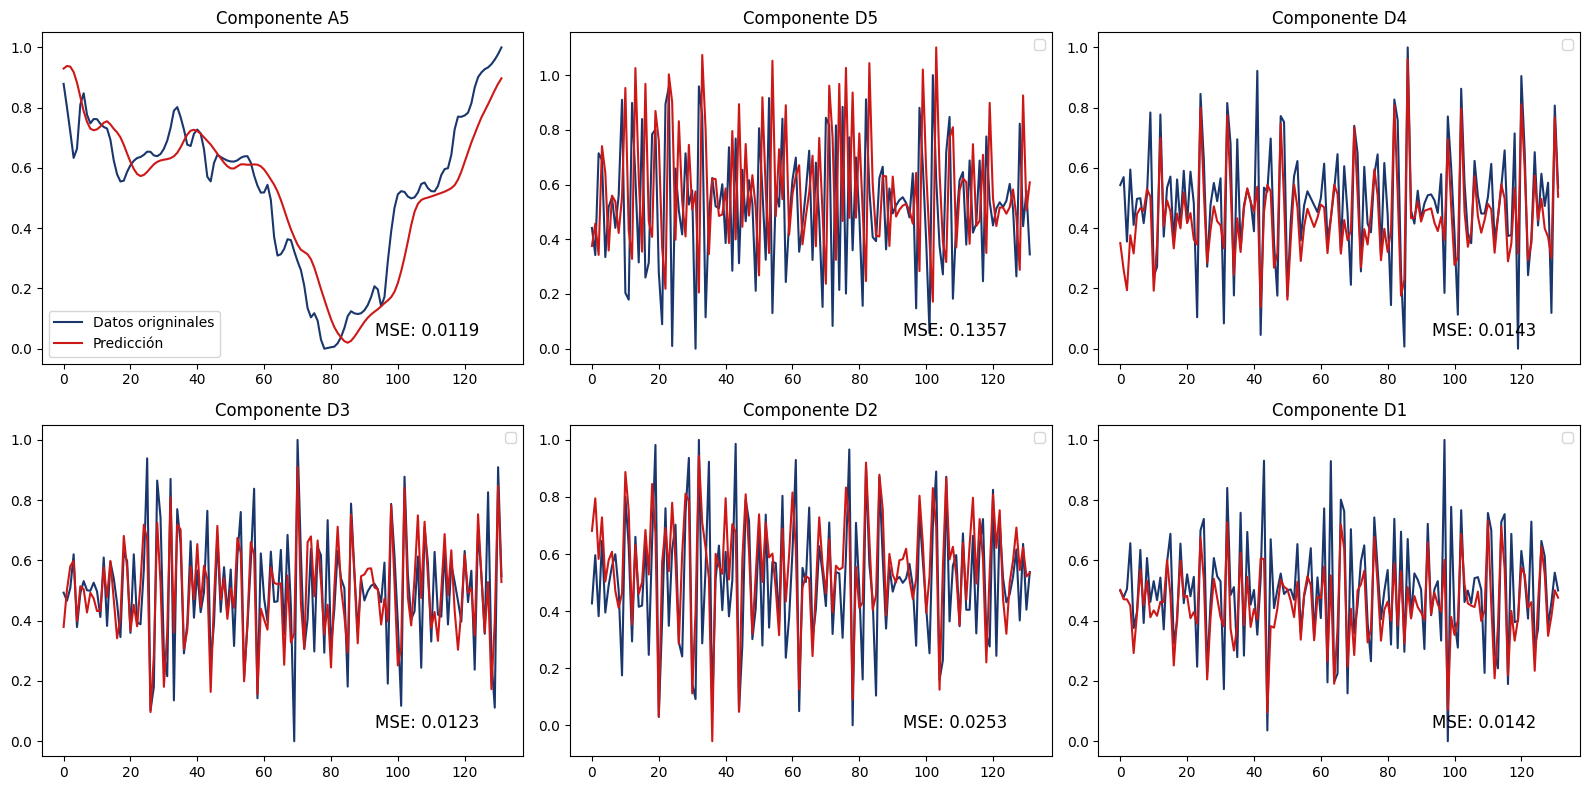
\includegraphics[width=0.9\textwidth]{Figuras/proceso_de_entrenamiento/grafs_c_prueba/muestreo_aleatorio/DWT_GRU/estandar/DWT_GRU.png}
    \caption{Predicciones de la DWT-GRUnn de los componentes del conjunto de pruebas de muestro aleatorio} 
    \label{fig:c_prueba_componentes_DWT_GRU_aleatorio}
\end{figure}

\begin{figure}[H]
    \centering
    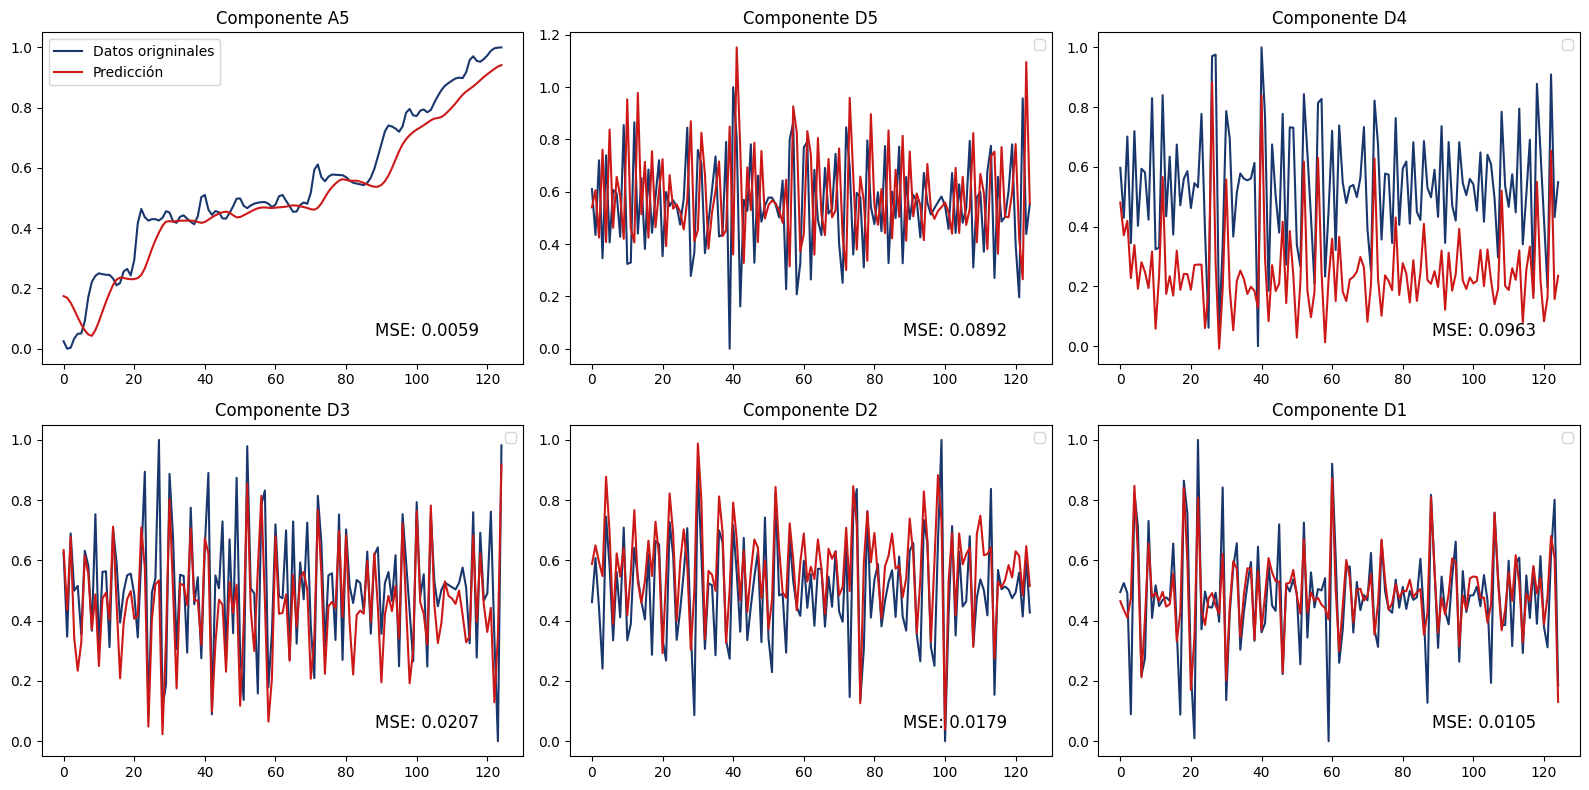
\includegraphics[width=0.9\textwidth]{Figuras/proceso_de_entrenamiento/grafs_c_prueba/DWT_GRU/estandar/DWT_GRU.png}
    \caption{Predicciones de la DWT-GRUnn de los componentes del conjunto de pruebas de muestro temporal} 
    \label{fig:c_prueba_componentes_DWT_GRU}
\end{figure}

Finalmente, y como ha ocurrido para los demás modelos que parten de redes recurrentes, se tomaron los mismos hiper-parametros para el DWT-GRUnn y se obtiene lo mostrado en las figuras \ref{fig:c_prueba_componentes_DWT_GRU_aleatorio} y \ref{fig:c_prueba_componentes_DWT_GRU}.

\begin{figure}[H]
    \begin{minipage}{0.5\textwidth}
        \centering
        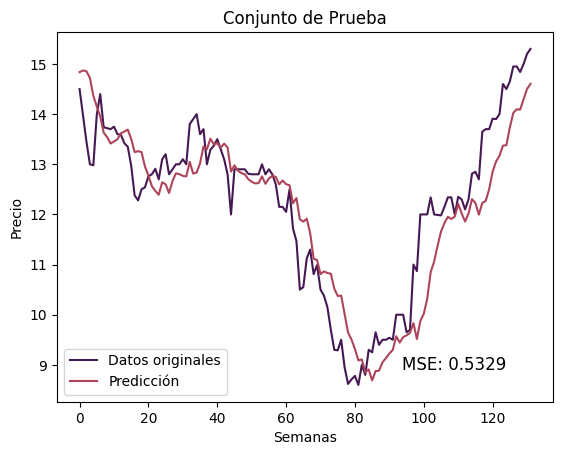
\includegraphics[width=\linewidth]{Figuras/proceso_de_entrenamiento/grafs_c_prueba/muestreo_aleatorio/DWT_GRU/estandar/DWT_GRU_rec.png}
    \end{minipage}
    \begin{minipage}{0.5\textwidth}
        \centering
        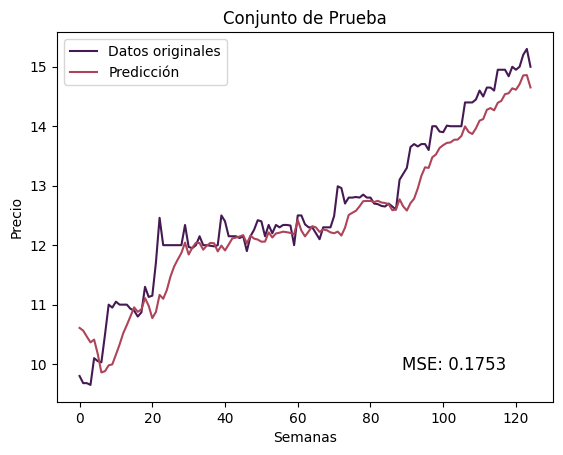
\includegraphics[width=\linewidth]{Figuras/proceso_de_entrenamiento/grafs_c_prueba/DWT_GRU/estandar/DWT_GRU_rec.png}
    \end{minipage}
    \caption{Desempeño de la DWT-GRUnn en la reconstrucción del conjunto de prueba: Muestro aleatorio y temporal.} 
    \label{fig:c_prueba_DWTGRU}
\end{figure}

Es bastante visible la mejoría que presenta la red GRU tanto en DWT-GRUnn como en GRUnn respecto a sus pares, en todas las predicciones el error disminuye y parece acercarse más a la serie original. Con o sin transformada de ondículas este enfoque de ANNs puede verse muy positivo para el pronostico de datos unidimensionales.

\newpage

\section{Entrenamiento Auto-predictivo}

De la misma manera que en la sección anterior, la entrada del conjunto de datos serán los precios de las primeras ocho semanas del conjunto de entrenamiento, para predecir el valor de la novena semana. Esa novena semana se concatenará como parte de la entrada en la predicción del precio siguiente semana, ocupando el lugar del octavo valor y repitiendo esto en las siguientes iteraciones. De esta forma, durante el cálculo de cada predicción se tomará como entrada a $[\hat{t}_{n-1}, \hat{t}_{n-2}, ..., \hat{t}_{n-8}]$ donde $\hat{t_i}$ es la predicción \textit{i-ésima} de la red, obteniendo $\hat{t_n}$. En la figura \ref{fig:entrenamiento_auto_predictivo} se puede ver en detalle la estructura de este enfoque.

\begin{figure}[h]
    \centering
    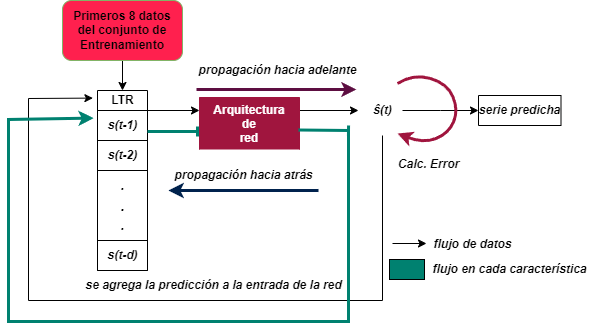
\includegraphics[width=0.8\textwidth]{Figuras/proceso_de_entrenamiento/Entrenamiento_auto_predictivo.png}
    \caption{Diagrama del entrenamiento auto-predictivo} 
    \label{fig:entrenamiento_auto_predictivo}
\end{figure}

Es importante recalcar que este experimento es de gran importancia para nuestro propósito, pues evaluará la autonomía de las redes para identificar tendencias de largo plazo. Sin embargo, no es el enfoque final del proyecto y se trata de un ambiente extremo al que se someten los modelos. Se toma un escenario para el cual el modelo solo dispone de ocho datos para predecir los consecuentes $n$ referentes al restante conjunto de datos. Con una información tan pequeña a disponer es imposible que se pueda mantener una predicción que pretenda ajustarse a un intervalo tan largo teniendo un punto de partida tan pequeño, pues el error que acarrea con las salidas predichas se acumula, y no es el objetivo predecir exactamente lo que sucederá, si no enfocarnos en cierta tendencia. Entonces, la finalidad de este análisis es puramente demostrativo, se busca encontrar qué modelo puede generar el mejor pronóstico en el peor escenario posible. 

%%%%%%%%%%%%%%%%%%%%%%%%%%%%%%%%%%%%%%%%%%%%%%%%%%%%%%%%%%%%%%%%%%%%%%
\subsection{NARNN}

La obtención de los hiper-parámetros de las redes ocurre de la misma manera analítica que en la subsección pasada. De esta forma, como se puede ver en la figura \ref{fig:lr_epocas_NARNN_autopred}, la mejor taza de aprendizaje y épocas son [0.0008,30].

\begin{figure}[H]
    \centering
    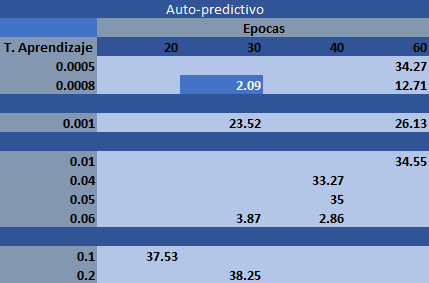
\includegraphics[width=0.5\textwidth]{Figuras/proceso_de_entrenamiento/lr_epocas_NARNN_auto_pred.png}
    \caption{Tabla comparativa entre parámetros de la NARNN: tasa de aprendizaje contra número épocas durante entrenamiento auto-predictivo.} 
    \label{fig:lr_epocas_NARNN_autopred}
\end{figure}

Con este entrenamiento, los pronósticos del conjunto de prueba son:

\begin{figure}[H]
    \begin{minipage}{0.5\textwidth}
        \centering
        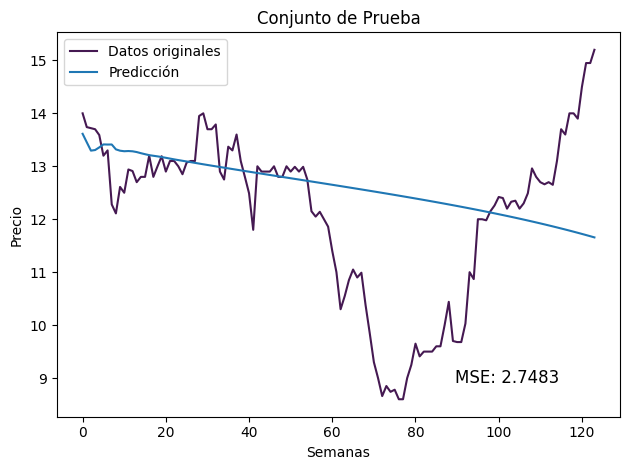
\includegraphics[width=\linewidth]{Figuras/proceso_de_entrenamiento/grafs_c_prueba/muestreo_aleatorio/NARNN/auto_predictiva/NARNN.png}
    \end{minipage}
    \begin{minipage}{0.5\textwidth}
        \centering
        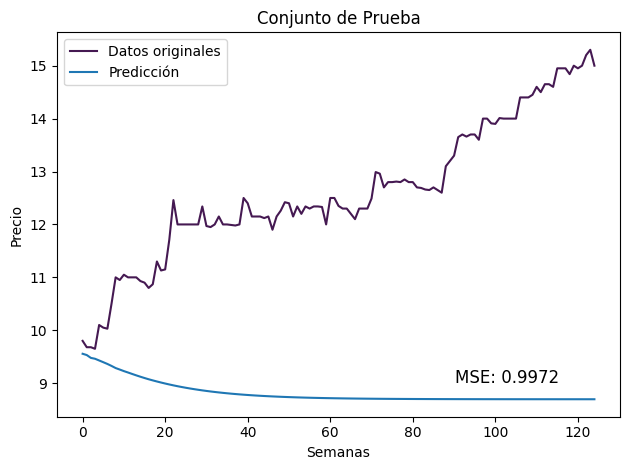
\includegraphics[width=\linewidth]{Figuras/proceso_de_entrenamiento/grafs_c_prueba/NARNN/auto_predictiva/NARNN.png}
    \end{minipage}
    \caption{Desempeño auto-predictivo de la NARNN en conjunto de prueba: Muestro aleatorio y temporal.} 
    \label{fig:c_prueba_NARNN_autopred_1}
\end{figure}

Vemos que en lo que respecta a la predicción, no encaja bien con los valores esperados. Esto surge desde que los primeros resultados de predicción arrastran consigo cierto error como se mencionaba más arriba y que, a la larga, este aumenta dándonos un resultado cada vez más inexacto. Por esta razón, se decidió agregar un nuevo parámetro, con el fin de estabilizar las primeras predicciones que la red nos da, de manera que los valores subsecuentes a estas se encuentren no tan alejadas al valor real.

Se empleó una técnica de decaimiento en la tasa de aprendizaje durante una época, de manera que en los lotes más próximos al inicio de la serie serán para los cuales la red aprenda mejor, garantizando que las predicciones en un inicio sean más acertadas y en consecuencia las siguientes arrastren una cantidad menor de error. \textit{El factor de decaimiento} (FD):

\begin{algorithm}[H]{
\caption{Ajuste del factor de decaimiento del aprendizaje}
\SetAlgoLined
\SetKwInOut{Input}{Entrada}
\SetKwInOut{Output}{Salida}

\SetKwFunction{onBatchBegin}{onBatchBegin}

%\Input{\textit{tasa actual}, \textit{lote}, \textit{tolerancia}, \textit{lote\_designado}}
%\Output{\textit{tasa actual}}

\BlankLine
\BlankLine

\SetKwProg{Fn}{alComenzarLote}{:}{}
    \Fn{(lote\_actual, perida\_actual)}{
        \BlankLine
            \If{perdida$\_$actual $\leq$ tolerancia \textbf{y} lote$\_$designado == lote$\_$actual}{
            factor$\_$de$\_$decaimiento = factor$\_$de$\_$decaimiento $\times$ 0.8\\
            %\tcp{Descomentar la siguiente línea si quieres imprimir el nuevo factor}
            %\tcp{print(f">>nuevo factor: {lr\_callback.decay\_factor}")}
            lote$\_$designado = lote$\_$designado + 1
            \BlankLine
            \tcp{El lote actual indica a partir de qué lote se empezará a tomar en cuenta el FD}
        }
        \BlankLine
        \textit{tasa\_actual}$ \gets \frac{\text{\textit{tasa\_inicial}}}{1 + \text{\textit{factor\_de\_decaimiento}} \times \text{\textit{iteracion}}}$ \tcp*{Calcula la nueva tasa de aprendizaje}
        \BlankLine
        %\textbf{Imprimir} "lr: ", lr, ", batch: ", batch \;
        \BlankLine
        \textit{iteracion}++ \tcp{Incrementa el número de iteración}
        %$\text{iteracion} \gets \text{iteracion} + 1$ \;
        \BlankLine
        \textbf{regresa} \textit{tasa\_actual} \;
    }
}
\end{algorithm}

Así, durante cada época si la pérdida actual es menor a la tolerancia y el lote designado es el actual, el FD cae, y la penalización de la tasa de aprendizaje en los siguientes lotes es menor. De cualquier forma se disminuye la tasa actual en función de la tasa inicial, el FD y el número de época o lote en el que nos encontramos.

Aplicando lo anterior, en la figura \ref{fig:lr_epocas_NARNN_autopred_v2} podemos ver un diagrama parecido a los anteriores, pero ahora considerando el FD como parte de la busqueda exahustiva de los hiper-parámetros.

\begin{figure}[H]
    \centering
    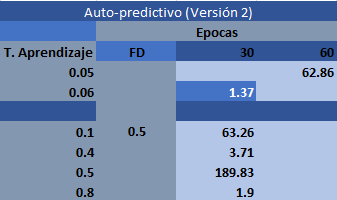
\includegraphics[width=0.5\textwidth]{Figuras/proceso_de_entrenamiento/lr_epocas_NARNN_auto_pred_v2.png}
    \caption{Tabla comparativa entre parámetros de la NARNN: tasa de aprendizaje contra número épocas y factor de decaimiento durante entrenamiento auto-predictivo.} 
    \label{fig:lr_epocas_NARNN_autopred_v2}
\end{figure}

\begin{figure}[h]
    \begin{minipage}{0.5\textwidth}
        \centering
        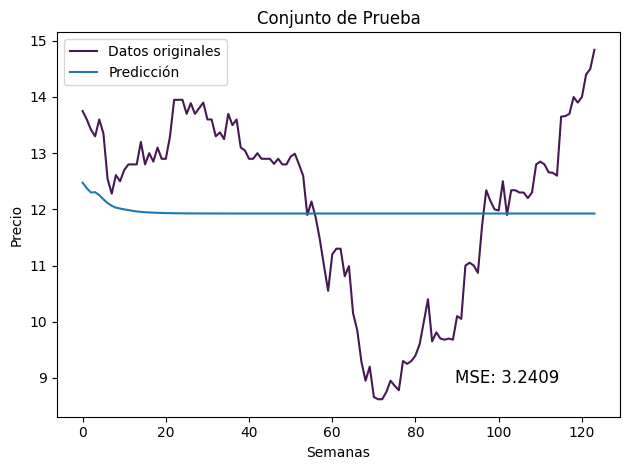
\includegraphics[width=\linewidth]{Figuras/proceso_de_entrenamiento/grafs_c_prueba/muestreo_aleatorio/NARNN/auto_predictiva/NARNN_v2.png}
    \end{minipage}
    \begin{minipage}{0.5\textwidth}
        \centering
        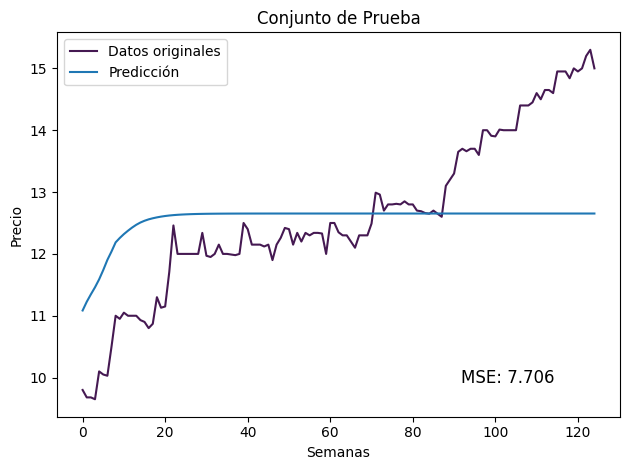
\includegraphics[width=\linewidth]{Figuras/proceso_de_entrenamiento/grafs_c_prueba/NARNN/auto_predictiva/NARNN_v2.png}
    \end{minipage}
    \caption{Desempeño auto-predictivo de la NARNN en conjunto de prueba bajo la implementación del factor de decaimiento: Muestro aleatorio y temporal.} 
    \label{fig:c_prueba_NARNN_autopred_v2}
\end{figure}

Encontrándonos así una mejor predicción en general \footnote{Notemos que esta técnica 'obliga' a la red a aprender mejor los primeros datos del conjunto en decremento de entendimiento que tiene de los subsecuentes. Hecho que perjudica a la predicción cualquier otro tipo de predicción que no sea enteramente auto-predictiva.}. Respecto al muestreo temporal, mejoró bastante, captando la tendencia creciente de los precios durante las primeras semanas, en contraposición de lo que se ve en el muestreo aleatorio que empeoro al inicio de las semanas.

%\newpage

%%%%%%%%%%%%%%%%%%%%%%%%%%%%%%%%%%%%%%%%%%%%%%%%%%%%%%%%%%%%%%%%%%%%%%
\subsection{DWT-NARNN}

En el mismo snetido, Se usaron los mismos parámetros que para la NARNN para el componente de baja frecuencia. Para los demás se encontró que un enfoque sin FD daba buen resultado.

\begin{figure}[H]
    \centering
    \includegraphics[width=0.5\textwidth]{Figuras/proceso_de_entrenamiento/lr_epocas_DWT_LSTM_auto_pred.png}
    \caption{Tabla comparativa entre parámetros de la DWT-NARNN para componentes de alta frecuencia: tasa de aprendizaje contra número épocas durante entrenamiento auto-predictivo.} 
    \label{fig:lr_epocas_DWTNARNN_autopred_v2}
\end{figure}

\begin{figure}[H]
    \centering
    \includegraphics[width=0.9\textwidth]{Figuras/proceso_de_entrenamiento/grafs_c_prueba/muestreo_aleatorio/DWT_NARNN/auto_predictiva/DWT_NARNN.png}
    \caption{Predicciones auto-predictivas de la DWT-NARNNnn de los componentes del conjunto de pruebas de muestro aleatorio.} 
    \label{fig:c_prueba_componentes_DWTNARNN_autopred_aleatorio}
\end{figure}

\begin{figure}[H]
    \centering
    \includegraphics[width=0.9\textwidth]{Figuras/proceso_de_entrenamiento/grafs_c_prueba/DWT_NARNN/auto_predictiva/DWT_NARNN.png}
    \caption{Predicciones auto-predictivas de la DWT-NARNNnn de los componentes del conjunto de pruebas de muestro temporal.} 
    \label{fig:c_prueba_componentes_DWTNARNN_autopred}
\end{figure}

\begin{figure}[H]
    \begin{minipage}{0.5\textwidth}
        \centering
        \includegraphics[width=\linewidth]{Figuras/proceso_de_entrenamiento/grafs_c_prueba/muestreo_aleatorio/DWT_NARNN/auto_predictiva/DWT_NARNN_rec.png}
    \end{minipage}
    \begin{minipage}{0.5\textwidth}
        \centering
        \includegraphics[width=\linewidth]{Figuras/proceso_de_entrenamiento/grafs_c_prueba/DWT_NARNN/auto_predictiva/DWT_NARNN_rec.png}
    \end{minipage}
    \caption{Desempeño auto-predictivo de la DWT-NARNNnn en conjunto de prueba: Muestro aleatorio y temporal.} 
    \label{fig:c_prueba_DWTNARNN_autopred_v2}
\end{figure}
%%%%%%%%%%%%%%%%%%%%%%%%%%%%%%%%%%%%%%%%%%%%%%%%%%%%%%%%%%%%%%%%%%%%%%
\newpage
\subsection{LSTMnn}

En el mismo sentido que la NARNN, los resultados del entrenamiento auto-predictivo sin implementar el factor de decaimiento no son muy alentadores.

\begin{figure}[H]
    \centering
    \includegraphics[width=0.45\textwidth]{Figuras/proceso_de_entrenamiento/lr_epocas_LSTM_auto_pred.png}
    \caption{Tabla comparativa entre parámetros de la LSTMnn: tasa de aprendizaje contra número épocas en un entrenamiento auto-predictivo.} 
    \label{fig:lr_epocas_LSTMnn_autopred}
\end{figure}

\newpage

Aplicando un estudio de la misma manera que la NARNN. Tenemos:

\begin{figure}[H]
    \centering
    \includegraphics[width=0.8\textwidth]{Figuras/proceso_de_entrenamiento/lr_epocas_LSTM_autopred_v2.png}
    \caption{Tabla comparativa entre parámetros de la LSTMnn: tasa de aprendizaje contra número épocas en un entrenamiento auto-predictivo con factor de decaimiento.} 
    \label{fig:lr_epocas_LSTMnn_autopred_v2}
\end{figure}

\begin{figure}[H]
    \begin{minipage}{0.5\textwidth}
        \centering
        \includegraphics[width=\linewidth]{Figuras/proceso_de_entrenamiento/grafs_c_prueba/muestreo_aleatorio/LSTM/auto_predictiva/LSTM_v2.png}
    \end{minipage}
    \begin{minipage}{0.5\textwidth}
        \centering
        \includegraphics[width=\linewidth]{Figuras/proceso_de_entrenamiento/grafs_c_prueba/LSTM/auto_predictiva/LSTM_v2.png}
    \end{minipage}
    \caption{Desempeño auto-predictivo de la LSTMnn en conjunto de prueba: muestreo aleatorio y temporal.} 
    \label{fig:c_prueba_LSTM_autopred_v2}
\end{figure}

\newpage

\subsection{DWT-LSTMnn}

Para este entrenamiento, se obtuvieron los siguientes resultados. 

\begin{figure}[H]
    \centering
    \includegraphics[width=0.6\textwidth]{Figuras/proceso_de_entrenamiento/lr_epocas_DWT_LSTM_auto_pred.png}
    \caption{Tabla comparativa entre parámetros de la DWT-LSTMnn: tasa de aprendizaje contra número épocas y factor de decaimiento durante entrenamiento auto-predictivo.} 
    \label{fig:lr_epocas_DWTLSTM_autopred_v2}
\end{figure}

Tomando la misma combinación de parámetros para las redes destinadas a cada componente.

\begin{figure}[H]
    \centering
    \includegraphics[width=0.9\textwidth]{Figuras/proceso_de_entrenamiento/grafs_c_prueba/muestreo_aleatorio/DWT_LSTM/auto_predictiva/DWT_LSTM.png}
    \caption{Predicciones auto-predictivas de la DWT-LSTMnn de los componentes del conjunto de pruebas de muestro aleatorio.} 
    \label{fig:c_prueba_componentes_DWTLSTM_autopred_aleatorio}
\end{figure}

\begin{figure}[H]
    \centering
    \includegraphics[width=0.9\textwidth]{Figuras/proceso_de_entrenamiento/grafs_c_prueba/DWT_LSTM/auto_predictiva/DWT_LSTM.png}
    \caption{Predicciones auto-predictivas de la DWT-LSTMnn de los componentes del conjunto de pruebas de muestro temporal.} 
    \label{fig:c_prueba_componentes_DWTLSTM_autopred}
\end{figure}

\begin{figure}[H]
    \begin{minipage}{0.5\textwidth}
        \centering
        \includegraphics[width=\linewidth]{Figuras/proceso_de_entrenamiento/grafs_c_prueba/muestreo_aleatorio/DWT_LSTM/auto_predictiva/DWT_LSTM_rec.png}
    \end{minipage}
    \begin{minipage}{0.5\textwidth}
        \centering
        \includegraphics[width=\linewidth]{Figuras/proceso_de_entrenamiento/grafs_c_prueba/DWT_LSTM/auto_predictiva/DWT_LSTM_rec.png}
    \end{minipage}
    \caption{Desempeño auto-predictivo de la DWT-LSTMnn en conjunto de prueba: muestreo aleatorio y temporal.} 
    \label{fig:c_prueba_DWTLSTM_autopred_v2}
\end{figure}

Durante las primeras semanas de la predicción, pareciera que LSTMnn y DWTLSTMnn siguen cierta tendencia de los datos originales, digamos unas diez semanas en el futuro. A pesar de esto vemos que ni las RNNs son capaces de mantener por tanto tiempo el pronóstico. Sin embargo, comparado con los modelos auto-regresivos, mejora notablemente al no usar siquiera la técnica FD.

\newpage

\subsection{GRUnn}

De la misma manera y parámetros que la LSTMnn:

\begin{figure}[H]
    \begin{minipage}{0.5\textwidth}
        \centering
        \includegraphics[width=\linewidth]{Figuras/proceso_de_entrenamiento/grafs_c_prueba/muestreo_aleatorio/GRU/auto_predictiva/GRU.png}
    \end{minipage}
    \begin{minipage}{0.5\textwidth}
        \centering
        \includegraphics[width=\linewidth]{Figuras/proceso_de_entrenamiento/grafs_c_prueba/GRU/auto_predictiva/GRU.png}
    \end{minipage}
    \caption{Desempeño auto-predictivo de la GRUnn en conjunto de prueba.} 
    \label{fig:c_prueba_GRU_autopred}
\end{figure}

%\newpage

\subsection{DWT-GRUnn}

De la misma manera y parámetros que la DWT-LSTMnn:

\begin{figure}[H]
    \centering
    \includegraphics[width=0.9\textwidth]{Figuras/proceso_de_entrenamiento/grafs_c_prueba/muestreo_aleatorio/DWT_GRU/auto_predictiva/DWT_GRU.png}
    \caption{Predicciones auto-predictivas de la DWT-GRUnn de los componentes del conjunto de pruebas de muestro aleatorio.} 
    \label{fig:c_prueba_componentes_DWTGRU_autopred_muestreo_aleatorio}
\end{figure}

\begin{figure}[H]
    \centering
    \includegraphics[width=0.9\textwidth]{Figuras/proceso_de_entrenamiento/grafs_c_prueba/DWT_GRU/auto_predictiva/DWT_GRU.png}
    \caption{Predicciones auto-predictivas de la DWT-LSTMnn de los componentes del conjunto de pruebas de muestro temporal.} 
    \label{fig:c_prueba_componentes_DWTGRU_autopred}
\end{figure}

\begin{figure}[H]
    \begin{minipage}{0.5\textwidth}
        \centering
        \includegraphics[width=\linewidth]{Figuras/proceso_de_entrenamiento/grafs_c_prueba/muestreo_aleatorio/DWT_GRU/auto_predictiva/DWT_GRU_rec.png}
    \end{minipage}
    \begin{minipage}{0.5\textwidth}
        \centering
        \includegraphics[width=\linewidth]{Figuras/proceso_de_entrenamiento/grafs_c_prueba/DWT_GRU/auto_predictiva/DWT_GRU_rec.png}
    \end{minipage}
    \caption{Desempeño auto-predictivo de la DWT-GRUnn en conjunto de prueba: muestreo aleatorio y temporal.} 
    \label{fig:c_prueba_DWTGRU_autopred_v2}
\end{figure}

Como se vió, los modelos no son aptos para este tipo de escenarios, pero los que han sido mejor evaluados, al menos durante las primeras semanas del análisis son sin duda los recurrentes. % Experiment 2

% !TEX root = ../Tesis.tex
\chapter{Evaluación de desempeño} 
\label{cap:evaluación de desempeño} 

En este capítulo se muestran los resultados que se obtuvieron en las métricas mencionadas. Para los modelos sin DWT se muestra únicamente el RMSE, MAPE y DS de la predicción del conjunto de prueba contra los precios reales. Para los restantes se pinta un desglose de cada medida por cada componente y la reconstrucción total del pronóstico del conjunto de pruebas.

\section{Predicción Estándar}

\begin{longtable}{lccc}
\textbf{NARNN | muestreo aleatorio} & \textbf{RMSE} & \textbf{MAPE (\%)} & \textbf{DS (\%)} \\
\textbf{Predicción de c\_prueba} & 1.014 & 7.21322 & 63.7097 \\
\textbf{DWT-NARNN | muestreo aleatorio} & & & \\
\textbf{Reconstrucción de c\_prueba} & 1.0769 & 7.397269 & 65.1515 \\
\textbf{Componente A5} & 1.0502 & 7.186337 & 62.8788 \\
\textbf{Componente D5} & 0.0000 & 133.993170 & 68.9394 \\
\textbf{Componente D4} & 0.0000 & 109.625883 & 62.8788 \\
\textbf{Componente D3} & 0.0000 & 102.676865 & 74.2424 \\
\textbf{Componente D2} & 0.0000 & 154.036830 & 70.4545 \\
\textbf{Componente D1} & 0.1402 & 315.594656 & 58.3333 \\

\textbf{LSTM | muestreo aleatorio} &  &  &  \\
\textbf{Predicción de c\_prueba} & 0.8335 & 6.015341 & 62.0968 \\
\textbf{DWT-LSTM | muestreo aleatorio} &  &  &  \\
\textbf{Reconstrucción de c\_prueba} & 0.8689 & 5.887960 & 68.1818 \\
\textbf{Componente A5} & 0.8488 & 5.699098 & 58.3333 \\
\textbf{Componente D5} & 0.0000 & 62.915075 & 81.0606 \\
\textbf{Componente D4} & 0.0000 & 95.984062 & 84.8485 \\
\textbf{Componente D3} & 0.0000 & 68.514078 & 79.5455 \\
\textbf{Componente D2} & 0.0000 & 69.674597 & 78.7879 \\
\textbf{Componente D1} & 0.1195 & 1924.748875 & 81.8182 \\

\textbf{GRU | muestreo aleatorio} &  &  &  \\
\textbf{Predicción de c\_prueba} & 0.7595 & 4.990504 & 68.5484 \\
\textbf{DWT-GRU | muestreo aleatorio} &  &  &  \\
\textbf{Reconstrucción de c\_prueba} & 0.7087 & 4.932105 & 70.4545 \\
\textbf{Componente A5} & 0.6824 & 4.713478 & 61.3636 \\
\textbf{Componente D5} & 0.0000 & 129.506225 & 40.9091 \\
\textbf{Componente D4} & 0.0000 & 125.145635 & 87.1212 \\
\textbf{Componente D3} & 0.0000 & 69.453592 & 82.5758 \\
\textbf{Componente D2} & 0.0000 & 62.306607 & 87.1212 \\
\textbf{Componente D1} & 0.1439 & 264.549962 & 83.3333 \\
\caption{Métricas de desempeño para muestro aleatorio}
\label{tab:resultados_prediccion_estandar_m_aleatorio}
    
\end{longtable}

Como se ve en la tabla \ref{tab:resultados_prediccion_estandar_m_aleatorio} el desempeño de NARNN y DWT-NARNN es bastante similar, pero peor con respecto a LSTM y DWT-LSTM, siendo esta última el que presenta una mejoría tanto en valores del error (RMSE, MAPE) como en la dirección (DS). En este sentido, los mejores son GRU y DWT-GRU. Así, durante este ejercicio, el modelo GRU ha demostrado una notable ventaja en predecir los valores con menor error, e incluso alcanza a llegar al 70\% en DS (recordemos que el pronóstico mejora el captar la dirección de la señal original a medida que esta medida se acerca al 100). A pesar de esto, se sigue analizando su desempeño. Ahora en la figura \ref{tab:resultados_prediccion_estandar_m_temporal} que se acerca más a nuestro objetivo final.

\begin{longtable}{lccc}

    \textbf{NARNN | muestreo temporal} & \textbf{RMSE} & \textbf{MAPE (\%)} & \textbf{DS (\%)} \\
\textbf{Predicción de c\_prueba} & 0.5272 & 3.728504 & 57.6 \\
\textbf{DWT-NARNN | muestreo temporal} &  &  &  \\
\textbf{Reconstrucción de c\_prueba} & 0.5421 & 3.895320 & 77.6 \\
\textbf{Componente A5} & 0.5234 & 3.788553 & 57.6 \\
\textbf{Componente D5} & 0.0000 & 174.387157 & 55.2 \\
\textbf{Componente D4} & 0.0000 & 154.766175 & 65.6 \\
\textbf{Componente D3} & 0.0000 & 107.227901 & 68.0 \\
\textbf{Componente D2} & 0.0000 & 204.159326 & 66.4 \\
\textbf{Componente D1} & 0.0987 & 445.400429 & 67.2 \\

\textbf{LSTM | muestreo temporal} &  &  &  \\
\textbf{Predicción de c\_prueba} & 0.4807 & 3.023597 & 58.4 \\
\textbf{DWT-LSTM | muestreo temporal} &  &  &  \\
\textbf{Reconstrucción de c\_prueba} & 0.4940 & 3.052687 & 71.2 \\
\textbf{Componente A5} & 0.5104 & 3.194822 & 50.4 \\
\textbf{Componente D5} & 0.0000 & 82.476074 & 77.6 \\
\textbf{Componente D4} & 0.0000 & 84.153618 & 80.8 \\
\textbf{Componente D3} & 0.0000 & 85.620667 & 76.0 \\
\textbf{Componente D2} & 0.0000 & 78.178528 & 80.0 \\
\textbf{Componente D1} & 0.0614 & 232.752878 & 76.0 \\

\textbf{GRU | muestreo temporal} &  &  &  \\
\textbf{Predicción de c\_prueba} & 0.4149 & 2.425552 & 58.4 \\
\textbf{DWT-GRU | muestreo temporal} &  &  &  \\
\textbf{Reconstrucción de c\_prueba} & 0.4186 & 2.538661 & 74.4 \\
\textbf{Componente A5} & 0.4200 & 2.560362 & 52.8 \\
\textbf{Componente D5} & 0.0000 & 165.702431 & 28.8 \\
\textbf{Componente D4} & 0.0000 & 271.978322 & 84.0 \\
\textbf{Componente D3} & 0.0000 & 84.694473 & 80.8 \\
\textbf{Componente D2} & 0.0000 & 101.649577 & 83.2 \\
\textbf{Componente D1} & 0.0507 & 162.795013 & 76.0 \\
\caption{Métricas de desempeño para muestro temporal}
\label{tab:resultados_prediccion_estandar_m_temporal}
\end{longtable}

Se tiene un comportamiento similar al ejercicio pasado, solo que los modelos en general han presentado una leve mejoría, siendo DWT-GRU y GRU mejores que DWT-LSTM y LSTM en predecir los valores puntuales y dirección.

A continuación, se analiza de la misma forma los resultados de los pronósticos durante la auto-predicción.

\section{Predicción Auto-regresiva}
%%%%%%%%%%%%%%%%%%%%%%%%%%%%%%%%%%%%%%%%%%%%%%%%%%%%%%%
%%%%%%%%%%%%%%%%%%%%%%%%%%%%%%%%%%%%%%%%%%%%%%%%%%%%%%%%%%%%

%\begin{table}[H]
  %\centering
  
  
\begin{longtable}{lccc}
  \textbf{NARNN | muestreo aleatorio} & \textbf{RMSE} & \textbf{MAPE (\%)} & \textbf{DS (\%)} \\
  \textbf{Predicción de c\_prueba} & 1.5902 & 11.690531 & 83.0645 \\
    \textbf{DWT-NARNN | muestreo aleatorio} & & & \\
    \textbf{Reconstrucción de c\_prueba} & 1.0769 & 7.397269 & 65.1515 \\
    \textbf{Componente A5} & 5.6517  & 47.323432 & 59.8485 \\
\textbf{Componente A5} & 5.6362  & 47.178851 & 56.0606 \\
\textbf{Componente D5} & 0.0000 & 100.315032 & 51.5152 \\
\textbf{Componente D4} & 0.0000  & 93.483034 & 47.7273 \\
\textbf{Componente D3} & 0.0000  & 87.791170 & 45.4545 \\
\textbf{Componente D2} & 0.0000 & 114.652779 & 55.3030 \\
\textbf{Componente D1} & 0.1212 & 126.322933 & 58.3333 \\


\textbf{LSTM | muestreo aleatorio} &  &  &  \\
    \textbf{Predicción de c\_prueba} & 1.5654 & 11.118145 & 56.4516 \\
\textbf{DWT-LSTM | muestreo aleatorio} &  &  &  \\
\textbf{Reconstrucción de c\_prueba} & 1.4242 & 10.028115 & 50.7576 \\
\textbf{Componente A5} & 1.4135 & 9.956542 & 45.4545 \\
\textbf{Componente D5} & 0.0000 & 89.239022 & 56.8182 \\
\textbf{Componente D4} & 0.0000 & 86.142969 & 40.1515 \\
\textbf{Componente D3} & 0.0000 & 97.384352 & 55.3030 \\
\textbf{Componente D2} & 0.0000 & 86.135574 & 58.3333 \\
\textbf{Componente D1} & 0.1619 & 562.130456 & 46.9697 \\

\textbf{GRU | muestreo aleatorio} &  &  &  \\
    \textbf{Predicción de c\_prueba} & 1.8843 & 14.017671 & 72.5806 \\
\textbf{DWT-GRU | muestreo aleatorio} &  &  &  \\
\textbf{Reconstrucción de c\_prueba} & 1.5201 & 11.193495 & 56.0606 \\
\textbf{Componente A5} & 1.5034 & 11.071481 & 45.4545 \\
\textbf{Componente D5} & 0.0000 & 79.033183 & 50.7576 \\
\textbf{Componente D4} & 0.0000 & 86.834054 & 70.4545 \\
\textbf{Componente D3} & 0.0000 & 88.958365 & 47.7273 \\
\textbf{Componente D2} & 0.0000 & 79.117372 & 53.0303 \\
\textbf{Componente D1} & 0.1516 & 137.442302 & 52.2727 \\
\caption{Métricas de desempeño para muestro aleatorio y predicción auto-predictiva}
\label{tab:resultados_prediccion_aregresiva_m_aleatorio}
\end{longtable}
  
%\end{table}
  
\begin{longtable}{lccc}
\textbf{NARNN | muestreo temporal} & \textbf{RMSE} & \textbf{MAPE (\%)} & \textbf{DS (\%)} \\
\textbf{Predicción de c\_prueba} & 1.1734 & 7.394705 & 76.8 \\

    \textbf{DWT-NARNN | muestreo temporal} & &  & \\
\textbf{Reconstrucción de c\_prueba} & 2.5790 & 16.083149 & 60.8 \\
\textbf{Componente A5} & 2.5705 & 16.032415 & 58.4 \\
\textbf{Componente D5} & 0.0000 & 103.209729 & 45.6 \\
\textbf{Componente D4} & 0.0000 & 101.234477 & 43.2 \\
\textbf{Componente D3} & 0.0000 & 92.928121 & 44.8 \\
\textbf{Componente D2} & 0.0000 & 106.261789 & 48.0 \\
\textbf{Componente D1} & 0.0867 & 166.880758 & 61.6 \\

\textbf{LSTM | muestreo temporal} & &  & \\
\textbf{Predicción de c\_prueba} & 1.134 & 6.435196 & 60.0 \\
\textbf{DWT-LSTM | muestreo temporal} &  &  &  \\
\textbf{Reconstrucción de c\_prueba} & 1.1875 & 6.243048 & 59.2 \\
\textbf{Componente A5} & 1.1900 & 6.227096 & 59.2 \\
\textbf{Componente D5} & 0.0000 & 94.481289 & 75.2 \\
\textbf{Componente D4} & 0.0000 & 92.125017 & 46.4 \\
\textbf{Componente D3} & 0.0000 & 79.400759 & 55.2 \\
\textbf{Componente D2} & 0.0000 & 96.781732 & 72.0 \\
\textbf{Componente D1} & 0.0885 & 193.398147 & 47.2 \\

\textbf{GRU | muestreo temporal} & &  & \\
\textbf{Predicción de c\_prueba} & 1.4637 & 8.468626 & 68.0 \\
\textbf{DWT-GRU | muestreo temporal} &  &  &  \\
\textbf{Reconstrucción de c\_prueba} & 1.3357 & 7.353046 & 60.0 \\
\textbf{Componente A5} & 1.3388 & 7.358327 & 60.0 \\
\textbf{Componente D5} & 0.0000 & 91.487306 & 46.4 \\
\textbf{Componente D4} & 0.0000 & 90.523456 & 57.6 \\
\textbf{Componente D3} & 0.0000 & 81.710255 & 46.4 \\
\textbf{Componente D2} & 0.0000 & 98.222451 & 44.0 \\
\textbf{Componente D1} & 0.0884 & 188.670092 & 53.6 \\
\caption{Métricas de desempeño para muestro temporal y predicción auto-predictiva}
\label{tab:resultados_prediccion_aregresiva_m_temporal}
\end{longtable}

Se esperaba que el desempeño de los modelos durante la auto-predicción sea peor. Como se mencionó antes, no es el objetivo del trabajo que estos operen en estos escenarios, pero gracias a este ejercicio se puede ver que tanto pueden predecir a lo largo del tiempo, y es precisamente por esto que vale la pena ahondar en él. En la tablas \ref{tab:resultados_prediccion_aregresiva_m_aleatorio} y \ref{tab:resultados_prediccion_aregresiva_m_temporal} se observa que los modelos con DWT son superiores en general al disminuir el error. Esto se debe a que al tener datos suavizados o simplificados, los modelos mantienen las predicciones más cercanas a la realidad por más tiempo ('arrastran' menos error), disminuyendo la perdida. Sin embargo los modelos sin ella nos brindan un mejor acercamiento a la dirección.

\newpage
%%%%%%%%%%%%%%%%%%%%%%%%%%%%%%%%%%%%%%%%%%%%%%%%%
\section{Predicción Auto-predictiva con Corrección}
%%%%%%%%%%%%%%%%%%%%%%%%%%%%%%%%%%%%%%%%%%%%

Hasta el momento, hemos trabajado con los datos de ACTINVRB durante 2016 a 2020, siendo que falta el análisis a los demás conjuntos. Por ello y para poner a prueba la capacidad de predicción de nuevas entradas de los modelos, emplearemos una esquema híbrido de predicción sobre los datos de las demás entidades financieras seleccionadas. Llamémosle \textit{Predicción Auto-predictiva con Corrección} al alimentar a los modelos con los valores de las últimas ocho semanas de cada conjunto de entrenamiento, generando ocho predicciones auto-predictivas, esto es, de la semana nueve hasta la dieciséis. Para la predicción de la semana diecisiete se toma nuevamente ocho entradas correspondientes que pertenecen a los datos reales y así sucesivamente en intervalos de ocho semanas. De este modo, generaremos pronósticos auto-predictivos y estándar alternados. Así logrando un esquema 'justo' en el cual los modelos se enfrentan a predicciones lo suficientemente autónomas para su evaluación. Entonces, se obtuvo lo siguiente para cada conjunto de datos.

\newpage

\begin{figure}[H]
    \centering
    \includegraphics[width=0.8\textwidth]{Figuras/analisis/NARNN.png}
    \caption{Desempeño del modelo NARNN} 
    \label{fig:desempenio_NARNN}
\end{figure}

\begin{figure}[H]
    \centering
    \includegraphics[width=0.8\textwidth]{Figuras/analisis/DWT_NARNN.png}
    \caption{Desempeño del modelo DWT-NARNN} 
    \label{fig:desempenio_DWTNARNN}
\end{figure}

\begin{figure}[H]
    \centering
    \includegraphics[width=0.8\textwidth]{Figuras/analisis/LSTM.png}
    \caption{Desempeño del modelo LSTM} 
    \label{fig:desempenio_LSTM}
\end{figure}

\begin{figure}[H]
    \centering
    \includegraphics[width=0.8\textwidth]{Figuras/analisis/DWT_LSTM.png}
    \caption{Desempeño del modelo DWT-LSTM} 
    \label{fig:desempenio_DWTLSTM}
\end{figure}

\begin{figure}[H]
    \centering
    \includegraphics[width=0.8\textwidth]{Figuras/analisis/GRU.png}
    \caption{Desempeño del modelo GRU} 
    \label{fig:desempenio_GRU}
\end{figure}

\begin{figure}[H]
    \centering
    \includegraphics[width=0.8\textwidth]{Figuras/analisis/DWT_GRU.png}
    \caption{Desempeño del modelo DWT-GRU} 
    \label{fig:desempenio_DWTGRU}
\end{figure}

Si se detiene el análisis un momento aquí, se ve en \ref{fig:desempenio_NARNN} y \ref{fig:desempenio_DWTNARNN} que las redes auto-regresivas tienden a sobrestimar los datos (como se ve en ACTINVRB, BOLSAA, GFINBURO y GNP) y a depender mucho de la 'correción' que ofrece este esquema híbrido cada ocho semanas. Vemos como las predicciones en ciertos puntos se alejan bastante de los valores reales y regresan abruptamente en intervalos de ocho semanas, formando estas estructuras con forma de cresta o pico cada cierto tiempo. Formas que no necesariamente son parte del comportamiento original de los datos.

Como se ve en \ref{fig:desempenio_DWTLSTM}, DWT-LSTM mejora la calidad de la predicción respecto a LSTM en \ref{fig:desempenio_LSTM}. La 'correción' que acurre cada ocho semanas se hace menos notoria, ya que los modelos mantienen su buen pronostico por más tiempo. Y en general la señal capta mejor la dirección que tomarán los precios. Ocurre algo similar en \ref{fig:desempenio_DWTGRU} y \ref{fig:desempenio_GRU} correspondientemente. Se observa que para las redes recurrentes es mucho más fácil captar las tendencias de la serie original, y con ayuda de la DWT permiten generar un resultado más cercano a este.

%%%%%%%%%%%%%%%%%%%%%%%%%%%%%%%%%%%%%%%%%%%%%%%%%%%%%%%%%%
%%%%%%%%%%%%%%%%%%%%%%%%%%%%%%%%%%%%%%%%%%%%%%%%%%%%%%%%%%

\subsection{Prueba de Kolmogorov-Smirnov}

Una métrica útil para comparar el desempeño de los modelos es la prueba estadística de Kolmogorov-Smirnov. Esta se enfoca en encontrar la diferencia máxima que existe entre dos distribuciones y así determinar si difieren significativamente entre si. Ya que no requiere asumir que los datos sigan una distribución específica, es sensible a las diferencias en las formas, como la posición, la dispersión y la forma general. Se puede valer de ella como menciona Hassani, H. y Silva, E \cite{kolmogorov}. En este caso se emplea para comparar la distribución de los errores (MSE) de las predicciones de cada modelo y de cada una se obtiene el estadístico $KS$ y el valor $p$. 

Como se observa en las figuras  \ref{fig:DWTNARNN_NARNN}, \ref{fig:DWTLSTM_LSTM}, \ref{fig:DWTGRU_GRU}, los estadísticos y valores $p$ son generados por la prueba bilateral y unilateral (medidas que se ven en el extremo inferior izquierdo de cada imagen). Para saber si existe una diferencia estadísticamente significativa el valor $p$ debe de ser menor a 0.05 en la prueba bilateral, así se rechaza la hipótesis nula y se acepta la alternativa. Y si la segunda distribución reporta un menor error estocástico debe de presentarse el mismo caso que en su homologa anterior pero en la prueba unilateral. 

Dicho lo anterior, Se obtuvo lo siguiente:

\begin{figure}[H]
    \centering
    \includegraphics[width=0.5\textwidth]{Figuras/analisis/kolmogorov/DWTNARNN_NARNN.png}
    \caption{Distribución de errores de predicción de los modelos DWT-NARNN vs. NARNN.} 
    \label{fig:DWTNARNN_NARNN}
\end{figure}

Se rechaza la hipótesis nula de la prueba bilateral y se acepta la alternativa ($2e-06 < 0.05$). Los errores no comparten la misma distribución, existe una diferencia estadísticamente significativa. Se acepta la hipótesis nula de la prueba unilateral ($0.0992 > 0.05$), el modelo NARNN reporta un menor error estocástico.

\begin{figure}[H]
    \centering
    \includegraphics[width=0.5\textwidth]{Figuras/analisis/kolmogorov/DWTLSTM_LSTM.png}
    \caption{Distribución de errores de predicción de los modelos DWT-LSTM vs. LSTM.} 
    \label{fig:DWTLSTM_LSTM}
\end{figure}

Se rechaza la hipótesis nula de la prueba bilateral y se acepta la alternativa ($0.6141 > 0.05$). Los errores no comparten la misma distribución, existe una diferencia estadísticamente significativa. 
Se acepta la hipótesis nula de la prueba unilateral ($0.3169 > 0.05$). el modelo DWT-LSTM reporta un menor error estocástico, debido a la prueba anterior, esta diferencia es mínima.

\begin{figure}[H]
    \centering
    \includegraphics[width=0.5\textwidth]{Figuras/analisis/kolmogorov/DWTGRU_GRU.png}
    \caption{Distribución de errores de predicción de los modelos DWT-GRU vs. GRU.} 
    \label{fig:DWTGRU_GRU}
\end{figure}

Se rechaza la hipótesis nula de la prueba bilateral y se acepta la alternativa ($0.0088 < 0.05$). Los errores no comparten la misma distribución, existe una diferencia estadísticamente significativa. Se rechaza la hipótesis nula de la prueba unilateral y se acepta la alternativa ($0.0044 < 0.05$). El modelo DWT-GRU reporta un menor error estocástico.

Como se ve, los modelos con menor error estocástico son NARNN, DWT-LSTM y DWT-GRU. A continuación en las figuras \ref{fig:NARNN_DWTGRU}, \ref{fig:NARNN_DWTLSTM} se muestra una comparativa entre los tres.

\begin{figure}[H]
    \centering
    \includegraphics[width=0.5\textwidth]{Figuras/analisis/kolmogorov/NARNN_DWTLSTM.png}
    \caption{Distribución de errores de predicción de los modelos NARNN vs. DWT-LSTM: El modelo DWT-LSTM reporta un menor error estocástico.} 
    \label{fig:NARNN_DWTLSTM}
\end{figure}

\begin{figure}[H]
    \centering
    \includegraphics[width=0.5\textwidth]{Figuras/analisis/kolmogorov/NARNN_DWTGRU.png}
    \caption{Distribución de errores de predicción de los modelos NARNN vs. DWT-GRU: El modelo DWT-GRU reporta un menor error estocástico.} 
    \label{fig:NARNN_DWTGRU}
\end{figure}

\begin{figure}[H]
    \centering
    \includegraphics[width=0.5\textwidth]{Figuras/analisis/kolmogorov/DWTGRU_DWTLSTM.png}
    \caption{Distribución de errores de predicción de los modelos DWT-GRU vs. DWT-LSTM: El modelo DWT-LSTM reporta un menor error estocástico.} 
    \label{fig:DWTGRU_DWTLSTM}
\end{figure}

Así, el modelo que muestra un menor error durante la prueba es el DWT-LSTM, un modelo recurrente con descomposición por ondículas.
\newpage
\subsection{Resultados finales}

%%%%%%%%%%%%%%%%%%%%%%%%%%%%%%%%%%%%%%%%%%%%%%%

\begin{figure}[H]
    \centering
    \includegraphics[width=0.6\textwidth]{Figuras/analisis/RMSE.png}
    \caption{Diagrama de caja para métrica RMSE de las predicciones de todos los conjuntos de datos.} 
    \label{fig:RMSE}
\end{figure}

\begin{figure}[H]
    \centering
    \includegraphics[width=0.6\textwidth]{Figuras/analisis/MAPE.png}
    \caption{Diagrama de caja para métrica MAPE de las predicciones de todos los conjuntos de datos.} 
    \label{fig:MAPE}
\end{figure}

\begin{figure}[H]
    \centering
    \includegraphics[width=0.6\textwidth]{Figuras/analisis/DS.png}
    \caption{Diagrama de caja para métrica DS de las predicciones de todos los conjuntos de datos.} 
    \label{fig:DS}
\end{figure}

Se organizan los resultados de las métricas durante los tres tipos diferentes de predicción. En el diagrama RMSE, las RNNs ya sea con DWT o no tienen un mejor desempeño de predicción que las NARNNs, un resultado que se esperaba ante el hecho de que las RNNs están capacitadas especialmente para resolver problemas de datos con dependencias a largo plazo como vimos en durante el estudio de redes neuronales.

Es importante destacar que a pesar de que la DWT sea una herramienta fundamentan en el desempeño de una red neuronal, la arquitectura y métodos de entrenamiento de esta son igualmente importantes. Como vimos a lo largo del estudio, la combinación de un pre-procesamiento de datos con una red recurrente nos brinda mejores resultados:

\begin{itemize}
    \item Podemos ver en el diagrama de cajón de RMSE que esta distribución es mayor cuando se usa la DWT (se equivoca más), pero es precisamente debido a la predicción de 'ruido' adicional en la serie, es decir, que al emplear la descomposición y la respectiva predicción en cada una de sus componentes y la posterior recomposición aumenta el ruido en esta y así consecuentemente el error o diferencia entre la serie original y esta. Hecho que no necesariamente significa que la predicción con DWT sea menor acertada, al contrario, la tendencia se ve mejor reflejada como podemos ver con el diagrama de DS.
    \item Los resultados de la predicción respecto a la dirección se adecuan más cuando existe la descomposición a diferencia de las redes que no cuentan con ella, es decir que cuando se usa la DWT, las tendencias de pérdida o ganancia son mejor captadas. Véase que los modelos con mejor desempeño con respecto a esta métrica son el par de GRUnns.
   
\end{itemize} % Results and Discussion

% !TEX root = ../Tesis.tex
\chapter{Conclusiones} 
\label{cap:conclusiones} 

Como se mencionó a lo largo del capitulo anterior, se ve en \ref{fig:RMSE} y \ref{fig:MAPE} que los modelos con DWT presentan mayor error, fenómeno que se explica entendiendo que los datos que predice cada una de las redes en las componentes de alta frecuencia agrega ruido a la red y aumenta el error de la reconstrucción. Esto podría sonar a que esta técnica solo ayuda que las redes se equivoquen, pero justamente ayudan a captar la tendencia de la dirección en la que se dirige. Las DWT ha permitido una mejora en la captación de tendencias en los datos a lo largo del tiempo, permitiendo que los modelos produzcan mejores resultados durante más tiempo. Sumado a lo anterior, las redes recurrentes superaron ampliamente a la red auto-regresiva, ya que durante todo el capitulo anterior mostraron tanto menor error en la predicción de valores como de dirección.

A lo largo del entrenamiento, se pudo comprobar que como bien señala Prudhviraju Srivatsavaya \cite{GRU_vs_LSTM}, gracias a que los parámetros y complejidad en una LSTMnn son mayores que en una GRUnn, el tiempo de entrenamiento es lógicamente mayor, hecho que suma un punto a favor de esta arquitectura. Con este análisis, podemos decir que el mejor paradigma fue el recurrente, empleando la DWT sobre la GRUnn.

%Sin embargo, no olvidemos que la predicción de precios de instrumentos financieros a lo largo del tiempo conlleva un reto importante y es vital no mantenerse atados a una sola tecnología cuando realizamos una investigación de este tipo. Existe una cantidad abismal de herramientas y técnicas que nos acercan cada día más a nuestros objetivos. Además de la creciente demanda de procesamiento de datos no dejemos de lado el análisis de otras variables sociales, políticas y culturales que impactan en estos estudios. Es por esta razón que este estudio no representa un cierre a la temática, si no que podemos encontrar en herramientas como la atención o modelos como los transformadores, buenos temas para continuar la investigación a futuro.

\subsection{Investigación a Futuro}

A partir de este punto, en futuras investigaciones, es importante explorar otros enfoques avanzados que han demostrado ser efectivos en la predicción de series de tiempo y precios de acciones. Modelos como las redes neuronales de atención y los transformadores (\textit{Transformer Networks}), que ya han sido revolucionarios en procesamiento de lenguaje natural, están ganando terreno en el análisis de secuencias financieras debido a su capacidad para captar dependencias a largo plazo y patrones más complejos. Además, se puede investigar la implementación de técnicas de aprendizaje por refuerzo (\textit{reinforcement learning}) para el desarrollo de estrategias para operaciones bursátiles adaptativas.

Asimismo, sería relevante integrar enfoques multimodales, combinando no solo datos históricos de precios, sino también variables ajenas a las matemáticas, como eventos políticos, cambios regulatorios, indicadores económicos, y análisis de sentimiento a partir de noticias o redes sociales. Estas variables externas pueden mejorar la capacidad de los modelos para predecir movimientos del mercado.

Finalmente, el uso de redes neuronales más avanzadas, como las Redes Neuronales Gráficas \textit{Graph Neural Networks} (GNNs) \cite{graphNN} para capturar las relaciones entre diferentes activos financieros también se presentan como prometedoras para futuras investigaciones. Esto permitiría desarrollar modelos que sean más robustos ante la volatilidad y que puedan adaptarse mejor a las condiciones cambiantes del mercado financiero.

\subsection{Proyecto a Futuro}

Como parte del trabajo a futuro y de la integración de este estudio a un proyecto de análisis financiero, se puede pensar en un servicio que combine una plataforma similar a la terminal de \textit{Bloomberg} con predicción de series de tiempo. Este podría ofrecer una herramienta poderosa para la extrapolación de precios de emisoras en mercados financieros que permitiera a inversionistas particulares información valiosa sobre sus compras.

\begin{figure}[H]
    \centering
    \includegraphics[width=1\textwidth]{Figuras/conclusiones/modelo_app.png}
    \caption{Bosquejo de ventana para predicción de datos.} 
    \label{fig:aplicacion}
\end{figure}

Una plataforma que permite a los usuarios acceder a datos financieros históricos y en tiempo real, y realizar predicciones sobre precios futuros de acciones, bonos u otros activos financieros utilizando no solo redes neuronales, sino otras técnicas que mencionadas en la sección anterior. Podría incluir:

\begin{enumerate}
    \item Acceso a predicciones personalizadas: Los usuarios podrían seleccionar emisoras específicas para recibir predicciones a corto y largo plazo basadas en los datos históricos.
    \item Visualización interactiva: Gráficos interactivos que muestran tanto datos históricos como predicciones futuras, con intervalos de confianza y métricas de precisión.
    \item Alertas y notificaciones: Los usuarios recibirían alertas cuando se predigan fluctuaciones importantes en los precios de activos.
\end{enumerate}

La fuente de los datos financieros partiría del consumo de datos de precios en tiempo real y datos históricos de varias fuentes confiables. En ese sentido, se valdría de:

\begin{enumerate}
    \item APIs de Datos Financieros: El servicio podría consumir datos desde APIs con un enfoque en obtener precios históricos, volumen, datos de mercado y otros indicadores financieros.
    \item Procesamiento y Limpieza de Datos: Una vez que los datos se obtienen de las APIs, serían preprocesados para eliminar valores faltantes, detectar anomalías y preparar los conjuntos de datos para ser usados por los modelos de predicción. Esto podría incluir transformaciones como la descomposición de series temporales.
\end{enumerate}

%3. Arquitectura del Servicio
Además, El servicio podría estar basado en una arquitectura distribuida, combinando varios componentes para manejar las predicciones en tiempo real y permitir la escalabilidad.

%a. Backend de Datos
%Este componente manejaría la recopilación y almacenamiento de los datos financieros. Podría incluir:

%Bases de datos relacionales (SQL): Para almacenar datos estructurados como precios históricos, información de las emisoras, o variables macroeconómicas.
%Bases de datos NoSQL (MongoDB, Cassandra): Para almacenar grandes volúmenes de datos no estructurados o semi-estructurados, como registros de transacciones en tiempo real.
%b. Módulo de Predicción
%El núcleo del sistema de predicción estaría compuesto por modelos de redes neuronales especializadas, como:

%LSTM (Long Short-Term Memory) y GRU: Estas son arquitecturas recurrentes adecuadas para la predicción de series de tiempo, debido a su capacidad para capturar patrones a largo plazo.
%Modelos Híbridos (CNN-LSTM, Transformers): Para mejorar la precisión, podrían implementarse arquitecturas híbridas que combinen convoluciones y recurrencias para capturar tanto patrones locales como globales.
%El servicio permitiría a los usuarios realizar predicciones de diferentes tipos:

El enfoque principal del pronostico con los modelos serían las predicciones a corto plazo con horizontes temporales de días o semanas. Sumadas a las predicciones basadas en patrones estacionales o tendencias a largo plazo.
%c. API REST para la Comunicación
%La aplicación podría utilizar una API REST para permitir que los usuarios y otros sistemas interactúen con el servicio de predicción. Esta API podría exponer varias funcionalidades, como:

%Solicitar predicciones para una emisora.
%Obtener datos históricos y en tiempo real.
%Visualizar gráficos de precios proyectados.
%d. Frontend de Usuario
%El frontend del sistema sería una interfaz web accesible a través de navegadores o aplicaciones móviles. El diseño debe ser intuitivo, con herramientas de visualización como:

%Gráficos de líneas y velas: Para mostrar precios históricos y predicciones.
%Panel de control personalizable: Para que los usuarios puedan gestionar sus emisoras favoritas y ver las predicciones relevantes.
%Señales y alertas: Donde el usuario pueda recibir notificaciones basadas en predicciones o eventos relevantes.
%e. Infraestructura en la Nube
%El servicio podría ser desplegado en la nube (AWS, Google Cloud, Microsoft Azure), lo que permitiría escalabilidad, alta disponibilidad y la capacidad de procesar grandes volúmenes de datos en tiempo real. Los modelos de predicción podrían ser servidos a través de microservicios, lo que permitiría una integración flexible y un despliegue continuo.

%4. Entrenamiento y Validación de Modelos
%El proceso de entrenamiento de los modelos implicaría:

%Entrenamiento con datos históricos: Los modelos serían entrenados con grandes volúmenes de datos históricos de precios de las emisoras y otros indicadores financieros (volumen, noticias económicas, etc.).
%Validación cruzada y prueba de modelos: Se usarían técnicas como la validación cruzada para evitar sobreajuste y garantizar que los modelos sean robustos y precisos.
%Ajuste de hiperparámetros: Se podrían emplear técnicas como la búsqueda en cuadrícula o el ajuste bayesiano para optimizar los hiperparámetros de los modelos.
%5. Organización del Desarrollo
%El desarrollo de un servicio de este tipo implicaría una organización clara de los equipos y las tareas:

%Equipo de Ingeniería de Datos: Encargado de la recopilación, limpieza y procesamiento de datos financieros.
%Equipo de Científicos de Datos: Responsable de diseñar, entrenar y ajustar los modelos de redes neuronales para la predicción.
%Equipo de Backend y APIs: Encargado de implementar la arquitectura del sistema, integrando la API REST y los microservicios necesarios.
%Equipo de DevOps: Para gestionar el despliegue, la escalabilidad y la infraestructura en la nube.
%Equipo de Frontend: Responsable de desarrollar la interfaz de usuario y las herramientas de visualización.
%6. Monetización y Escalabilidad
%Este servicio podría monetizarse a través de suscripciones, donde los usuarios paguen por acceso a predicciones premium, más detalladas o con mayor frecuencia de actualización. También podría ofrecerse como una API para empresas interesadas en incorporar predicciones a sus propios sistemas.

En cuanto a la escalabilidad, los modelos de predicción deben actualizarse constantemente con nuevos datos, lo que necesitaría de un sistema robusto para gestionar grandes cantidades de información y realizar inferencias rápidas en tiempo real.

Este servicio ofrecería un enfoque nuevo para análisis financiero, combinando datos en tiempo real con técnicas avanzadas de predicción de series de tiempo para mejorar la precisión de las predicciones en mercados volátiles, con una arquitectura flexible y escalable en la nube.  % Conclusion

%% ----------------------------------------------------------------
% Now begin the Appendices, including them as separate files

\addtocontents{toc}{\vspace{2em}} % Add a gap in the Contents, for aesthetics

\appendix % Cue to tell LaTeX that the following 'chapters' are Appendices

% !TEX root = ../Tesis.tex
\chapter{Desarrollo del gradiente \texorpdfstring{$o_t$}{ot} y \texorpdfstring{$a_o$}{ao}}
\label{ApA}

Para $o_t$:

$\dfrac{E}{o_t} = \dfrac{\partial E}{\partial h_t} \cdot \dfrac{\partial h_t}{\partial o_t}$, por regla de la cadena

$\Longrightarrow \dfrac{E}{o_t} = \dfrac{\partial E}{\partial h_t} \cdot \dfrac{\partial}{\partial o_t} (o_t \cdot \tanh(c_t))$, sustituyendo el valor de $h_t$

$\Longrightarrow \dfrac{E}{o_t} = \dfrac{\partial E}{\partial h_t} \cdot \tanh(c_t)$

Y para $a_o$:

$\dfrac{E}{\partial a_o} = \dfrac{\partial E}{\partial o_t} \cdot \dfrac{\partial o_t}{\partial a_o}$

$\Longrightarrow \dfrac{E}{\partial a_o} = \dfrac{\partial E}{\partial o_t} \cdot \dfrac{\partial}{\partial a_o} (\sigma (a_o))$

$\Longrightarrow \dfrac{E}{\partial a_o} = \dfrac{\partial E}{\partial o_t} \cdot \sigma (a_o)(1-\sigma(a_o)$

$\Longrightarrow \dfrac{E}{\partial a_o} = \dfrac{\partial E}{\partial h_t} \cdot \tanh(c_t) \cdot o_t(1-o_t)$ 	% Appendix Title

% !TEX root = ../Tesis.tex
\chapter{Implementación de algoritmos}
\label{ApB}

\section{DWT multinivel}

\begin{lstlisting}[language=Python]
import pywt

def multilevel_dwt(data,wavelet,levels,mode = 'constant'):
    """
    Calcula la transformada de ondicula (wavelet) de un conjunto de datos o serie de tiempo y devuelve sus componentes
    [IMPORTANTE] cAn, cDn hacen referencia a los coeficientes de aprocimacion y detalle al nivel n respectivamente, que surgen de la descomposicion de la serie por 
    la transformada, mientras que An y Dn son los componentes de aproximacion y detalle al nivel n, se generan al aplicar una reconstruccion parcial (upcoef) de 
    los coeficientes y son utiles para, al sumar cada uno de estos componentes, obtener la senial original.
    Args:
        data: serie o senial a descomponer
        wavelet: funcion con la cual se realizara la convolucion, y en consecuencia la descomposicion
        levels: nivel de la descomposicion
        mode:
    """
    n = len(data)
    componentes = []
    At = data

    for l in range(1,levels+1):
        # descompone la serie de tiempo en un siguiente nivel y obtiene los coeficientes de detalle y aproximacion
        (cAt, cDt) = pywt.dwt(At, wavelet, mode)
        # componentes de Aproximacion 
        At = pywt.upcoef('a', cAt, wavelet, take = n)
        # componentes de Detalle
        Dt = pywt.upcoef('d', cDt, wavelet, take = n)
        componentes[:0] = [Dt]
        if (l == levels):
            componentes[:0] = [At]
    return componentes
\end{lstlisting}

\section{Implementación NARNN}

\begin{lstlisting}[language=Python]
import torch.nn as nn
import torch.nn.functional as F

class NARNN(nn.Module):
    """
    Red Neuronal no Lineal Auto-regresiva
    
    Estructura de la red:
        Entrada: los n valores anteriores de un instante de la serie.
        Arquitectura: 3 capas densamente conectadas con 10 neuronas cada una. La primera con la funcion tangente-sigmode 
        y la segunda con logaritmo-sigmoide como funciones de activacion. Luego la capa de salida,
        con una funcion lineal como activacion comprende una sola neurona. 
        Salida: un solo valor que representa la semana consecuente a las n de entrada.
    """
    def __init__(self, t_entrada, t_salida, nombre = 'NARNN'):
        super(NARNN, self).__init__()
        self.nombre = nombre
        self.fc1 = nn.Linear(t_entrada,10)
        self.fc2 = nn.Linear(10,10)
        self.fc3 = nn.Linear(10,t_salida)

    def forward(self, x):
        """
        Paso de propagacion hacia adelante de la red
        """
        tan_sigmoid = lambda a : F.tanh(F.sigmoid(a))
        x = tan_sigmoid(self.fc1(x))
        x = F.logsigmoid(self.fc2(x))
        x = self.fc3(x)
        return x
\end{lstlisting}

\section{Implementación LSTMnn}

\begin{lstlisting}[language=Python]
from keras import Model
from keras.layers import LSTM
from keras.layers import Dropout
from keras.layers import Dense

class red_LSTM(Model):
    """
    Red Neuronal con celdas de Memoria de Corto y Largo Plazo
    
    Estructura de la red:
        Entrada: los n valores anteriores de un instante de la serie.
        Arquitectura: 4 capas con 50 celdas LSTM e intercaladas 4 capas de desactivacion (dropout)
        del 20% y finalmente una ultima capa densamente conectada que comprende una sola neurona. 
        Salida: un solo valor que representa la semana consecuente a las n de entrada.
    """
    def __init__(self,input_dim,output_dim):
        super().__init__()#red_LSTM,self
        self.LSTM1 = LSTM(units=50,return_sequences=True,input_shape=(input_dim, 1))
        self.dropout1 = Dropout(0.2)
        self.LSTM2 = LSTM(units=50,return_sequences=True)
        self.dropout2 = Dropout(0.2)
        self.LSTM3 = LSTM(units=50,return_sequences=True)
        self.dropout3 = Dropout(0.2)
        self.LSTM4 = LSTM(units=50)
        self.dropout4 = Dropout(0.2)
        self.dense = Dense(units=output_dim)

    def call(self, inputs):
        """
        Define el comportamiento del modelo cuando se llama.
        """
        x = self.LSTM1(inputs)
        x = self.dropout1(x)
        x = self.LSTM2(x)
        x = self.dropout2(x)
        x = self.LSTM3(x)
        x = self.dropout4(x)
        x = self.LSTM4(x)
        x = self.dropout4(x)
        return self.dense(x)
\end{lstlisting}

\section{Implementación GRUnn}

\begin{lstlisting}[language=Python]
from keras import Model
from keras.layers import GRU
from keras.layers import Dropout
from keras.layers import Dense

class red_GRU(Model):
    """
    Red Neuronal con Unidades Recurrentes Cerradas
    
    Estructura de la red:
        Entrada: los n valores anteriores de un instante de la serie.
        Arquitectura: 4 capas con 50 celdas LSTM e intercaladas 4 capas de desactivaciOn (dropout)
        del 20% y finalmente una Ultima capa densamente conectada que comprende una sola neurona. 
        Salida: un solo valor que representa la semana consecuente a las n de entrada.
    """
    def __init__(self,input_dim,output_dim):
        super().__init__()#red_GRU,self
        self.GRU1 = GRU(units=50,return_sequences=True,input_shape=(input_dim, 1))
        self.dropout1 = Dropout(0.2)
        self.GRU2 = GRU(units=50,return_sequences=True)
        self.dropout2 = Dropout(0.2)
        self.GRU3 = GRU(units=50,return_sequences=True)
        self.dropout3 = Dropout(0.2)
        self.GRU4 = GRU(units=50)
        self.dropout4 = Dropout(0.2)
        self.dense = Dense(units=output_dim)

    def call(self, inputs):
        """
        Define el comportamiento del modelo cuando se llama.
        """
        x = self.GRU1(inputs)
        x = self.dropout1(x)
        x = self.GRU2(x)
        x = self.dropout2(x)
        x = self.GRU3(x)
        x = self.dropout4(x)
        x = self.GRU4(x)
        x = self.dropout4(x)
        return self.dense(x)
\end{lstlisting}

\section{Algoritmo Levenberg-Marquardt}

\begin{lstlisting} [language=Python]
    def step(self):
        """
        Paso de la optimizacion del algoritmo LM
        """
        x_n = self.aux_convierte_parametros() 

        #calculamos la matriz hessiana
        h = torch.autograd.functional.hessian(self.calcula_perdida, x_n) 

        #calculamos el gradiente de la funcion
        grad_f = torch.autograd.grad(self.calcula_perdida(x_n), x_n)[0]

        # calculamos la transpuesta del gradiente
        grad_f = torch.transpose(torch.unsqueeze(grad_f, 0),0, 1) 

        # multiplica un escalar por la matriz identidad del tamanio de h y se lo sumamos a h
        h_p = h+self.lambda*torch.eye(h.size(1))
        #producto punto entre - la inversa de h_p y el gradiente de la red
        x_n1 = torch.matmul(-torch.inverse(h_p),grad_f) 
        #se le da la forma adecuada para que se pueda sumar con el vector de nuevos pesos
        x_n = x_n.reshape(h.size(1), 1)

        #se realiza la actualizacion a los parametros
        x_n = x_n + self.lr*x_n1 
        return self.asigna_parametros(torch.transpose(x_n,0,1)[0],reasignar=False)
\end{lstlisting}
 % Appendix Title

% !TEX root = ../Tesis.tex
\chapter{Especificaciones de software}
\label{ApC}

\begin{table}[htbp]
  \centering
  \caption{Paquetes y sus versiones}
  \begin{tabular}{lll}
    \toprule
    \textbf{Paquete} & \textbf{Versión} \\
    \midrule
    keras                        & 2.13.1 \\
    matplotlib                   & 3.8.3 \\
    matplotlib-inline            & 0.1.6 \\
    numpy                        & 1.24.3 \\
    pandas                       & 2.2.1 \\
    pywavelets                   & 1.5.0 \\
    scikit-learn                 & 1.4.1.post1 \\
    scipy                        & 1.12.0 \\
    tensorboard                  & 2.13.0 \\
    tensorboard-data-server      & 0.7.2 \\
    tensorflow                   & 2.13.1 \\
    tensorflow-estimator         & 2.13.0 \\
    tensorflow-intel             & 2.13.1 \\
    tensorflow-io-gcs-filesystem & 0.31.0 \\
    torch                        & 2.2.1 \\
    torch-tb-profiler            & 0.4.3 \\
    torchaudio                   & 2.2.1 \\
    torchvision                  & 0.17.1 \\
    \bottomrule
  \end{tabular}
\end{table}

\begin{table}[htbp]
  \centering
  \caption{Especificaciones del dispositivo}
  \begin{tabular}{ll}
    \toprule
    \textbf{Procesador} & 13th Gen Intel(R) Core(TM) i7-13700HX @ 2.10 GHz \\
    \textbf{RAM instalada} & 32.0 GB (31.6 GB utilizable) \\
    \textbf{Tipo de sistema} & Sistema operativo de 64 bits, procesador x64 \\
    \bottomrule
  \end{tabular}
\end{table}
 % Appendix Title

\addtocontents{toc}{\vspace{2em}}  % Add a gap in the Contents, for aesthetics
\backmatter

%% ----------------------------------------------------------------
\label{Bibliography}
\setstretch{1} % Less spacing is accepted for the items in the bibliography.
\lhead{\emph{Bibliografía}}  % Change the left side page header to "Bibliography"
\bibliographystyle{unsrtnat}  % Use the "unsrtnat" BibTeX style for formatting the Bibliography
\bibliography{Bibliografia}  % The references (bibliography) information are stored in the file named "Bibliography.bib"

\end{document}
